%%%%%%%% ICML 2026 EXAMPLE LATEX SUBMISSION FILE %%%%%%%%%%%%%%%%%

\documentclass{article}

% Recommended, but optional, packages for figures and better typesetting:
\usepackage{microtype}
\usepackage{graphicx}
\usepackage{subcaption}
\usepackage{booktabs} % for professional tables

% hyperref makes hyperlinks in the resulting PDF.
% If your build breaks (sometimes temporarily if a hyperlink spans a page)
% please comment out the following usepackage line and replace
% \usepackage{icml2026} with \usepackage[nohyperref]{icml2026} above.
\usepackage{hyperref}
\usepackage[inline]{enumitem}
\usepackage{listings}
\usepackage{siunitx}
\usepackage{float}
\usepackage{longtable}
\usepackage{multirow}


% Attempt to make hyperref and algorithmic work together better:
\newcommand{\theHalgorithm}{\arabic{algorithm}}

% Use the following line for the initial blind version submitted for review:
% \usepackage{icml2026}

% For preprint / arXiv, use:
\usepackage[preprint]{icml2026}

% If accepted, instead use the following line for the camera-ready submission:
% \usepackage[accepted]{icml2026}

\usepackage{amsmath}
\usepackage{amssymb}
\usepackage{mathtools}
\usepackage{amsthm}
\usepackage{multirow}
\usepackage{xurl}
\usepackage{caption}
% \usepackage{polski}
% same purpose but keep format stable
\usepackage[T1]{fontenc}
\usepackage[utf8]{inputenc}


% if you use cleveref..
\usepackage[capitalize,noabbrev]{cleveref}
\definecolor{posgreen}{rgb}{0.13,0.54,0.13}
\definecolor{negred}{rgb}{0.80,0.20,0.15}
\newcommand{\ppos}[1]{\textcolor{posgreen}{+#1}}
\newcommand{\nneg}[1]{\textcolor{negred}{--#1}}
\newcommand{\pzero}[1]{\textcolor{gray}{#1}}
\usepackage{additional_macros}

%%%%%%%%%%%%%%%%%%%%%%%%%%%%%%%%
% THEOREMS
%%%%%%%%%%%%%%%%%%%%%%%%%%%%%%%%
\theoremstyle{plain}
\newtheorem{theorem}{Theorem}[section]
\newtheorem{proposition}[theorem]{Proposition}
\newtheorem{lemma}[theorem]{Lemma}
\newtheorem{corollary}[theorem]{Corollary}
\theoremstyle{definition}
\newtheorem{definition}[theorem]{Definition}
\newtheorem{assumption}[theorem]{Assumption}
\theoremstyle{remark}
\newtheorem{remark}[theorem]{Remark}
\newcommand{\benchmarkName}{\textsc{SkillsBench}}


% Todonotes is useful during development; simply uncomment the next line
%    and comment out the line below the next line to turn off comments
%\usepackage[disable,textsize=tiny]{todonotes}
\usepackage[textsize=tiny]{todonotes}
\newcommand{\sh}[1]{\textcolor{orange}{[shenghan: #1]}}
% The \icmltitle you define below is probably too long as a header.
% Therefore, a short form for the running title is supplied here:
\icmltitlerunning{SkillsBench: Benchmarking How Well Agent Skills Work Across Diverse Tasks}

% Redefine plain pagestyle to have no header/footer/rules (for first page)
\fancypagestyle{plain}{\fancyhf{}\renewcommand{\headrulewidth}{0pt}}

\begin{document}

\twocolumn[
  % \icmltitle{Submission and Formatting Instructions for \\
    % International Conference on Machine Learning (ICML 2026)}
    \icmltitle{SkillsBench: Benchmarking How Well Agent Skills Work Across Diverse Tasks}
  % It is OKAY to include author information, even for blind submissions: the
  % style file will automatically remove it for you unless you've provided
  % the [accepted] option to the icml2026 package.

  % List of affiliations: The first argument should be a (short) identifier you
  % will use later to specify author affiliations Academic affiliations
  % should list Department, University, City, Region, Country Industry
  % affiliations should list Company, City, Region, Country

  % You can specify symbols, otherwise they are numbered in order. Ideally, you
  % should not use this facility. Affiliations will be numbered in order of
  % appearance and this is the preferred way.
  \icmlsetsymbol{equal}{*}
  \icmlsetsymbol{outsideamazon}{\dag}

  \begin{icmlauthorlist}
    % Lead
    \icmlauthor{Xiangyi Li$^\ast$}{benchflow}
    % ~30 points co-first-authors
    \icmlauthor{Yimin Liu$^\ast$}{osu}
    \icmlauthor{Wenbo Chen$^\ast$}{amazon,outsideamazon}
    \icmlauthor{Shenghan Zheng$^\ast$}{dartmouth}
    % ~24 points core authors
    \icmlauthor{Xiaokun Chen$^\ddagger$}{stanford}
    \icmlauthor{Yifeng He$^\ddagger$}{ucdavis}
    \icmlauthor{Yubo Li$^\ddagger$}{cmu}
    \icmlauthor{Bingran You$^\ddagger$}{ucberkeley}
    % ~20 points core authors
    % reviewed all bibs
    \icmlauthor{Haotian Shen$^\ddagger$}{independent}
    \icmlauthor{Jiankai Sun$^\ddagger$}{independent}
    \icmlauthor{Shuyi Wang$^\ddagger$}{independent}
    % 19 points
    \icmlauthor{Binxu Li}{princeton}
    \icmlauthor{Qunhong Zeng}{independent}
    \icmlauthor{Di Wang}{foxconn}
    % 18 points
    \icmlauthor{Xuandong Zhao}{ucberkeley}
    % 17 points
    \icmlauthor{Yuanli Wang}{bu}
    % 16 points
    \icmlauthor{Roey Ben Chaim}{zenity}
    % 12 points (alphabetical by last name)
    \icmlauthor{Zonglin Di}{ucsc}
    \icmlauthor{Yipeng Gao}{usc}
    \icmlauthor{Junwei He}{bytedance}
    \icmlauthor{Yizhuo He}{cmu}
    \icmlauthor{Liqiang Jing}{utdallas}
    \icmlauthor{Luyang Kong}{independent}
    \icmlauthor{Xin Lan}{msu}
    \icmlauthor{Jiachen Li}{utaustin}
    \icmlauthor{Songlin Li}{stanford}
    \icmlauthor{Yijiang Li}{ucsd}
    \icmlauthor{Yueqian Lin}{duke}
    \icmlauthor{Xinyi Liu}{independent}
    \icmlauthor{Xuanqing Liu}{independent}
    \icmlauthor{Haoran Lyu}{independent}
    \icmlauthor{Ze Ma}{columbia}
    \icmlauthor{Kaixin Li}{independent}
    \icmlauthor{Runhui Wang}{independent}
    \icmlauthor{Tianyu Wang}{independent}
    \icmlauthor{Wengao Ye}{oxford}
    \icmlauthor{Yue Zhang}{utdallas}
    % Other contributions
    \icmlauthor{Hanwen Xing}{independent}   \icmlauthor{Kaixin Li}{independent}
    \icmlauthor{Yiqi Xue}{usc}
    % Advising
    \icmlauthor{Steven Dillmann}{stanford}
    \icmlauthor{Han-chung Lee}{independent}
  \end{icmlauthorlist}

  \icmlaffiliation{benchflow}{BenchFlow}
  \icmlaffiliation{amazon}{Amazon}
  \icmlaffiliation{osu}{Ohio State University}
  \icmlaffiliation{dartmouth}{Dartmouth College}
  \icmlaffiliation{stanford}{Stanford University}
  \icmlaffiliation{ucdavis}{UC Davis}
  \icmlaffiliation{cmu}{Carnegie Mellon University}
  \icmlaffiliation{ucberkeley}{UC Berkeley}
  \icmlaffiliation{independent}{Independent}
  \icmlaffiliation{princeton}{Princeton University}
  \icmlaffiliation{foxconn}{Foxconn}
  \icmlaffiliation{bu}{Boston University}
  \icmlaffiliation{zenity}{Zenity}
  \icmlaffiliation{ucsc}{UC Santa Cruz}
  \icmlaffiliation{usc}{USC}
  \icmlaffiliation{bytedance}{ByteDance}
  \icmlaffiliation{utdallas}{UT Dallas}
  \icmlaffiliation{msu}{Michigan State University}
  \icmlaffiliation{utaustin}{UT Austin}
  \icmlaffiliation{duke}{Duke University}
  \icmlaffiliation{oxford}{University of Oxford}
  \icmlaffiliation{ucsd}{UC San Diego}
  \icmlaffiliation{columbia}{Columbia University}
  \icmlcorrespondingauthor{Xiangyi Li}{xiangyi@benchflow.ai}

  % You may provide any keywords that you find helpful for describing your
  % paper; these are used to populate the "keywords" metadata in the PDF but
  % will not be shown in the document
  \icmlkeywords{Machine Learning, Agent Skills, Benchmarking}

  \vskip 0.15in

% Abstract centered in full-width area
\begin{center}
\begin{minipage}{0.92\textwidth}
\centerline{\textbf{\large Abstract}}
\vskip 0.1in
\small
Agent Skills are structured packages of procedural knowledge that augment LLM agents at inference time. Despite rapid adoption, there is no standard way to measure whether they actually help. We present \benchmarkName{}, a benchmark of 86 tasks across 11 domains paired with curated Skills and deterministic verifiers. Each task is evaluated under three conditions: no Skills, curated Skills, and self-generated Skills. We test 7 agent-model configurations over 7,308 trajectories. Curated Skills raise average pass rate by 16.2 percentage points (pp), but effects vary widely by domain (+4.5pp for Software Engineering to +51.9pp for Healthcare) and 16 of 84 tasks show negative deltas. Self-generated Skills provide no benefit on average, showing that models cannot reliably author the procedural knowledge they benefit from consuming. Focused Skills with 2--3 modules outperform comprehensive documentation, and smaller models with Skills can match larger models without them. We publish the dataset and evaluation harness to assist developers and researchers in future work at \href{https://www.skillsbench.ai/}{skillsbench.ai}.
\end{minipage}
\end{center}

\vskip 0.2in

% Figure in full-width area (side-by-side layout for single column)
\centerline{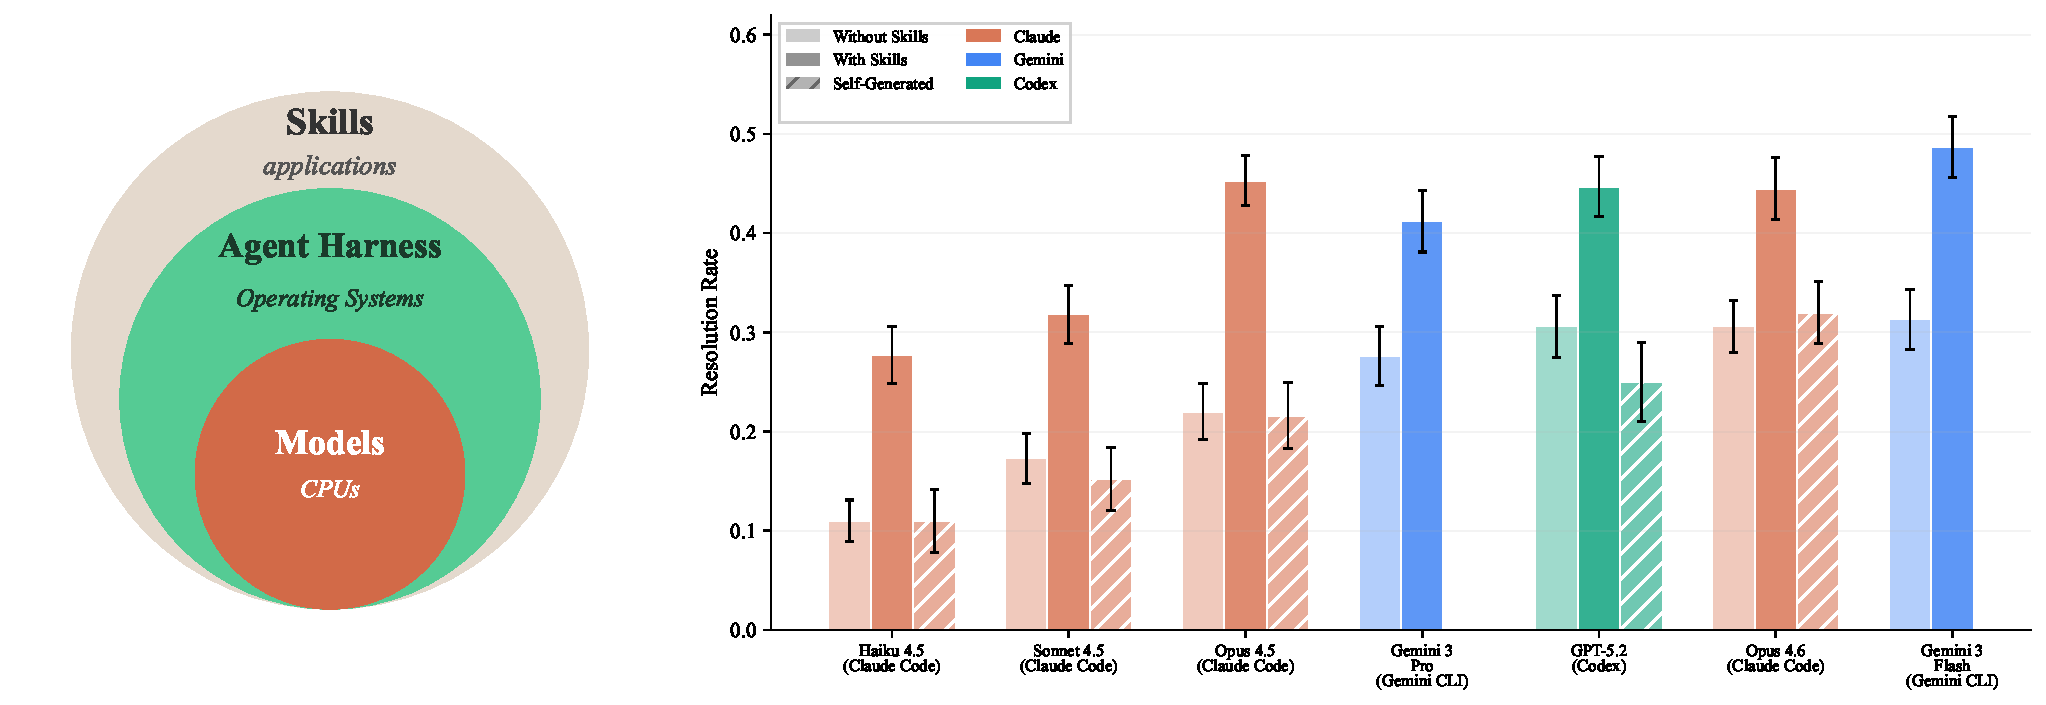
\includegraphics[width=0.95\textwidth]{figs/stacked_sidebyside.pdf}}
\vskip 0.08in
\centerline{\small \textbf{Figure 1:} Agent architecture stack and resolution rates across 7 agent-model configurations on 84 tasks.}
\centerline{\small Curated Skills (beige) improve performance by +16.2pp on average; self-generated Skills (amber) provide negligible or negative benefit.}
\phantomsection\label{fig:architecture}

\vskip 0.15in
]

% Set figure counter since we manually placed Figure 1 above
\setcounter{figure}{1}


% this must go after the closing bracket ] following \twocolumn[ ...

% This command actually creates the footnote in the first column listing the
% affiliations and the copyright notice. The command takes one argument, which
% is text to display at the start of the footnote. The \icmlEqualContribution
% command is standard text for equal contribution. Remove it (just {}) if you
% do not need this facility.

% Use ONE of the following lines. DO NOT remove the command.
% If you have no special notice, KEEP empty braces:
\printAffiliationsAndNotice{\textit{$^\ast$Equal contribution. $^\ddagger$Core contribution. \dag{}This work was conducted outside the author's role at Amazon.}}


\section{Introduction}
\label{sec:intro}

Large language models (LLMs) have evolved from text generators into autonomous agents capable of executing complex, multi-step tasks in real-world environments~\citep{brown2020languagemodelsfewshotlearners, chowdhery2022palmscalinglanguagemodeling, touvron2023llamaopenefficientfoundation, ouyang2022training, yao2023reactsynergizingreasoningacting}.
This evolution is exemplified by agent-centric CLI tools: Claude Code~\citep{anthropic2025claudecode} from Anthropic, Gemini CLI~\citep{google2025geminicli} from Google, and Codex CLI~\citep{openai2025codexcli} from OpenAI enable developers to leverage frontier models as agentic assistants within terminal environments.
However, a fundamental tension exists: foundation models provide broad capabilities but lack the procedural knowledge required for domain-specific workflows, while fine-tuning is expensive and sacrifices generality.

\textbf{Agent Skills} offer an emerging solution.
A Skill is a structured package comprising instructions, code templates, resources, and verification logic that augments agent behavior at inference time without model modification~\citep{anthropic2025agentskills}.
Skills encode procedural knowledge: standard operating procedures, domain conventions, and task-specific heuristics that guide agent behavior.
This modular approach builds on the options framework for temporal abstraction~\citep{sutton1999between} and cognitive architectures for language agents~\citep{sumers2024cognitive}, mirroring successful computing paradigms: foundation models provide base capabilities (analogous to CPUs), agent harnesses orchestrate context and tools (operating systems), and Skills extend competence to specialized domains (applications).
%This modular approach builds on the options framework for temporal abstraction~\citep{sutton1999between} and cognitive architectures for language agents~\citep{sumers2024cognitive}.
%This architecture mirrors successful computing paradigms: foundation models provide base capabilities (analogous to CPUs), agent harnesses orchestrate context and tools (operating systems), and Skills extend competence to specialized domains (applications).

% Figure 1 moved to main.tex (page 1, full-width)

% Skills ecosystems have grown rapidly, with community repositories now hosting thousands of user-contributed Skills spanning software engineering, data analysis, and enterprise workflows. Yet despite this proliferation, no benchmark systematically evaluates how and when Skills improve agent performance, what content drives gains, or what design principles distinguish effective Skills from ineffective ones. The question is not whether adding task-relevant context helps, but rather: How much do Skills help compared to baseline augmentation? Which Skills components (instructions vs.\ code vs.\ examples) contribute most? When do Skills fail despite being present?

Skills ecosystems have grown rapidly, with community repositories now hosting thousands of user-contributed Skills spanning software engineering, data analysis, and enterprise workflows. Yet despite this proliferation, no benchmark systematically evaluates how and when Skills improve agent performance, what content drives gains, or what design principles distinguish effective Skills from ineffective ones. \autoref{fig:architecture} illustrates this layered architecture and previews our main result: curated Skills consistently improve resolution rates across all 7 model-harness configurations, while self-generated Skills provide negligible benefit. The question is not whether adding task-relevant context helps, but rather: \textit{How much do Skills help compared to baseline augmentation? Which Skills components (instructions vs.\ code vs.\ examples) contribute most? When do Skills fail despite being present?}

%The growth of Skills ecosystems has been rapid---community repositories now host thousands of user-contributed Skills spanning software engineering, data analysis, and enterprise workflows (see Appendix~\ref{app:ecosystem} for ecosystem analysis).
%Yet despite this proliferation, a critical gap exists: \emph{no benchmark systematically evaluates how and when Skills improve agent performance, what types of Skills content drive gains, or what design principles distinguish effective Skills from ineffective ones}.
%The question is not \emph{whether} adding task-relevant context helps---that is nearly tautological---but rather: How much do Skills help compared to baseline augmentation? Which Skills components (instructions vs.\ code vs.\ examples) contribute most? When do Skills fail despite being present?

Existing agent benchmarks~\citep{liu2023agentbench, merrill2026terminalbenchbenchmarkingagentshard, jimenez2024swebench, zhou2024webarena, xie2024osworld, koh2024visualwebarena, trivedi2024appworld, yang2023intercode, chan2025mlebench, zhuo2025bigcodebench} evaluate raw model capabilities in isolation, answering \textit{``How well can this model perform task X?''} but not \textit{``How much does Skills Y improve performance on task X?''} This gap has practical consequences: practitioners cannot make informed decisions about Skills adoption, and researchers lack empirical grounding for Skills design principles.
%This methodological gap has practical consequences: practitioners cannot make informed decisions about which Skills to adopt, and researchers lack the empirical foundation to study Skills design principles.

To address this, we introduce \benchmarkName{}, the first benchmark that treats Skills as first-class evaluation artifacts, with two core contributions:
\begin{enumerate}[nosep,leftmargin=*]
\item \textbf{A Skills-centric evaluation framework.} We curate 84 tasks across 11 domains, each executed under three conditions---no Skills, curated Skills, and self-generated Skills---with deterministic verifiers and full trajectory logging. We stratify tasks by difficulty and conduct leakage audits to ensure Skills provide guidance rather than solutions.

\item \textbf{Large-scale empirical evaluation.} We evaluate 7 agent-model configurations across 7,308 trajectories, producing the first systematic evidence on Skills efficacy, variance, and failure modes.

% \item \textbf{Actionable findings that challenge conventional wisdom.} Skills help on average (+14.4 points) but hurt on nearly a third of tasks. Compact Skills sets (2--3) outperform comprehensive libraries. Smaller models with Skills can surpass larger models without. These results establish design principles for Skills authors and deployment strategies for practitioners.

\end{enumerate}
%\textbf{(1) Paired Evaluation Protocol.}
%Every task in SkillsBench is evaluated under multiple conditions: a \emph{vanilla} baseline (no Skills) and \emph{Skills-augmented} conditions with varying Skills content (L1: $\sim$6\%, L2: $\sim$10\%, L3: full, plus a BYOS condition).
%This paired design enables direct measurement of Skills efficacy---the delta between conditions---controlling for model capability, task difficulty, and evaluation infrastructure.

% \textbf{(2) Difficulty-Stratified Task Suite.}
% We curate 85 tasks across 13 domains stratified by expected human completion time: Easy ($<$15 minutes, 6 tasks), Medium (1--4 hours, 52 tasks), and Hard ($>$4 hours, 27 tasks).
% This stratification, validated with intrinsic difficulty metrics (dependency depth, tool invocations, state complexity), enables analysis of how Skills efficacy varies with task complexity.

% \textbf{(3) Leakage Prevention and Skills Quality Control.}
% To prevent Skills from encoding task-specific solutions, we establish authoring guidelines, conduct leakage audits measuring Skills-solution similarity (n-gram overlap, semantic similarity, command overlap), and document Skills quality variance.
% Skills with similarity metrics $>$0.30 were revised or excluded.


% Our evaluation comprises two experiments across \num{6970} valid trajectories. \textbf{Experiment 1} tests 6 LLMs across 5 agent harnesses (Claude Code, Gemini CLI, Codex, Terminus-2, Terminus-2-Skills) in 14 configurations on all 85 tasks, comparing with/without Skills. \textbf{Experiment 2} analyzes Skills design factors including quantity, complexity, and domain effects. Key findings:

% \begin{itemize}[leftmargin=*,itemsep=2pt,topsep=2pt]
%     \item \textbf{Variable Skills Benefit:} Skills yield +14.4pp average improvement but with high variance (+7.7pp to +26.9pp). Codex + GPT-5.2 achieves maximum performance (49.5\%).
%     \item \textbf{Skills Can Hurt Performance:} Software Engineering shows --5.0pp delta; 24 of 85 tasks exhibit negative Skills effects, suggesting domain-specific deployment strategies are needed.
%     \item \textbf{Optimal Skills Quantity:} 2--3 Skills provides +20.0pp improvement; 4+ Skills shows diminishing returns (+5.2pp). Compact Skills (+18.9pp) outperform comprehensive ones (+5.7pp).
%     \item \textbf{Reliability Issues:} Skills-aware harness variants (Terminus-2-Skills) show 31.7--65.3\% exception rates, revealing that aggressive Skills prompting can destabilize execution.
%     \item \textbf{Model Scale Effects:} Haiku + Skills (25.2\%) exceeds Opus without Skills (23.6\%) on procedural tasks, demonstrating Skills can partially compensate for model capacity.
% \end{itemize}

% \noindent\textbf{Scope and Limitations.}
% SkillsBench focuses on terminal-based agentic tasks where Skills provide procedural guidance.
% We do not claim to benchmark all forms of agent augmentation or all task domains.
% Our contribution is methodological: demonstrating that paired evaluation reveals insights invisible to single-condition benchmarks.
% We acknowledge that Skills injection adds tokens, and additional control baselines (random text of equivalent length, retrieved documentation) would strengthen causal claims---we discuss this limitation in \S\ref{sec:discussion}.

\section{\benchmarkName{}}
\label{sec:SkillsBench}

We present \benchmarkName{}, a benchmark for evaluating the efficacy of \emph{Skills augmentation} in LLM-based agents. Built on the Harbor framework~\citep{merrill2026terminalbenchbenchmarkingagentshard, harborframeworkteam2026harborframework}, each task adopts a containerized structure with an environment that includes agent Skills and related data, a deterministic verification test, and an oracle solution. Following best practices for agentic benchmarks~\citep{zhu2025bestpractices, anthropic2026demystifying}, we ensure strict isolation and deterministic verification. Unlike Terminal-Bench, which evaluates raw model and agent harness capability, \benchmarkName{} introduces a key methodological difference: we evaluate every task under both \emph{vanilla} (no Skills) and \emph{Skills-augmented} conditions, enabling direct measurement of Skills efficacy.

\subsection{Skills Specification}
\label{sec:skill_spec}

A \textbf{Skill} is an artifact that satisfies four criteria:
\begin{itemize}[nosep,leftmargin=*]
    \item \textbf{Procedural content}: Contains how-to guidance (procedures, workflows, SOPs), not factual retrieval
    \item \textbf{Task-class applicability}: Applies to a class of problems, not a single instance
    \item \textbf{Structured components}: Includes a \texttt{SKILL.md} file plus optional resources (scripts, templates, examples)
    \item \textbf{Portability}: Skills are soley based on file systems, so it's easy to edit, version, share, and be used across different skills-compatible agent harnesses. 
\end{itemize}

\noindent This definition explicitly \emph{excludes}: system prompts (lack structure and resources), few-shot examples~\citep{brown2020languagemodelsfewshotlearners} (declarative, not procedural), RAG retrievals~\citep{lewis2021retrievalaugmentedgenerationknowledgeintensivenlp} (factual, not procedural), and tool documentation~\citep{schick2023toolformerlanguagemodelsteach, qin2024toolllm} (describes capabilities, not procedures).
We acknowledge this boundary is not absolute
(for example, a StackOverflow answer may blend factual and procedural content),
but our criteria provide operational clarity for benchmark construction.
We highlight the distinguishing features of Skills compared to other augmentation paradigms in \autoref{tab:comparison}.


% \paragraph{Skills Structure.}
In \benchmarkName{}, each Skill is a modular package located in \texttt{environment/skills/} containing:
\begin{itemize*}%[nosep,leftmargin=*]
    \item \texttt{SKILL.md}: Natural language instructions specifying \emph{how} to approach a class of tasks,
    i.e., workflows, standard operating procedures, or domain conventions.
    \item \textbf{Resources}: Executable scripts, code templates, reference documentation, or worked examples that the agent may invoke or consult.
\end{itemize*}

% \paragraph{Comparison with Related Concepts.}
% Table~\ref{} distinguishes Skills from related augmentation paradigms.

\begin{table}[t]
\centering
\small
\caption{Comparison of runtime augmentation paradigms. Skills uniquely combine modular packaging with procedural guidance and optional executable resources, while remaining portable across models and harnesses.}
\label{tab:comparison}
\begin{tabular}{lcccc}
\toprule
& \textbf{Prompts} & \textbf{RAG} & \textbf{Tools} & \textbf{Skills} \\
\midrule
Modular/reusable & \texttimes & \checkmark & \checkmark & \checkmark \\
Procedural guidance & Limited & \texttimes & \texttimes & \checkmark \\
Executable resources & \texttimes & \texttimes & \checkmark & \checkmark \\
Cross-model portable & \checkmark & \checkmark & \checkmark & \checkmark \\
\bottomrule
\end{tabular}
\end{table}

\subsection{Task Specification}

Each task in \benchmarkName{} is a self-contained module comprising four components:
% \vspace{-1.95em}
\begin{itemize}[nosep,leftmargin=*]
\item \textbf{Instruction.} A human-readable task description specifying the objective, input format, and expected output. We write instructions to be solvable by a knowledgeable human without access to the paired Skills, though the Skills may substantially reduce time-to-solution.

\item \textbf{Environment.} A Docker container with task-specific data files and a \texttt{skills/} subdirectory containing modular Skills packages. The container ensures reproducibility through isolated dependencies and clean file system state.

\item \textbf{Solution.} A reference implementation demonstrating the task's resolvability. This oracle validates that each task has at least one correct solution path.

\item \textbf{Verifier.} Deterministic test scripts with programmatic assertions, including numeric tolerances where appropriate. This ensures reproducible pass/fail determination without LLM-as-a-judge variance, following execution-based evaluation best practices~\citep{wang2023execution, brown_verifiers_2025}.
\end{itemize}
\subsection{Dataset Construction}
The expressive and flexible nature of Skills and our task specifications enables broad coverage across diverse domains and problem types such as ....
To maximize this diversity, we adopted a \textbf{community-driven, open-source contribution model}: 105 contributors from both academia and industry submitted 322 candidate tasks.
We count submissions that included the full task specification
(instruction, environment, solution, and verifier),
along with author-assessed difficulty ratings.
From this pool, we curated the final \benchmarkName{} dataset. 
% through a rigorous two-stage selection process. 

% \subsection{Quality Control}

\subsection{Contributing Principles}
Contributors must satisfy explicit requirements designed to ensure task quality and prevent shortcuts:

\paragraph{Human-Authored Instructions.}
Task instructions must be written by humans, not generated by language models. We enforce this because LLMs generated queries will be confined by the distributions of LLMs, which are the subject of our evaluations, and LLM-generated queries are most of the time of low quality. 

\paragraph{Skill Generality.}
Skills must provide procedural guidance for a \emph{class} of tasks, not solutions to specific instances. Instructions must not reference which Skills to use, meaning agents must discover and apply Skills autonomously. This ensures we measure genuine Skill utilization rather than instruction-following.

\paragraph{Deterministic Verification.}
All success criteria must be testable through programmatic assertions. We target minimal number of tests needed for verification, avoiding both insufficient coverage and redundant test bloat that leads to artifical low pass rates. Tests must include informative error messages and use parametrization rather than duplication.

\paragraph{Automated Validation.}
Each submission undergoes automated validation before human review:
\begin{itemize}[nosep,leftmargin=*]
    \item \textbf{Structural validation}: Required files present (\texttt{instruction.md}, \texttt{task.toml}, \texttt{solve.sh}, \texttt{test\_outputs.py}), correct directory layout, valid TOML/YAML syntax.
    \item \textbf{Oracle execution}: Reference solution must achieve 100\% test pass rate. Tasks with failing oracles are rejected.
    \item \textbf{Instruction quality}: Instruction must be human written (we apply both human review and GPTZero review, and we achieve human label on 100\% of our tasks). We also evaluate instructions by six criteria (explicit output paths, structured requirements, success criteria, constraints listed, context-first ordering).
\end{itemize}

\paragraph{Human Review.}
After automated checks pass, maintainers conduct manual review evaluating five criteria:
(1) \emph{data validity}: input data must reflect real-world complexity; synthetic or toy data is rejected unless justified;
(2) \emph{task realism}: scenarios must reflect realistic professional workflows without artificial difficulty;
(3) \emph{oracle quality}: reference solutions should match how domain experts would solve the task;
(4) \emph{Skill quality}: Skills must be error-free, internally consistent, and genuinely useful for similar tasks beyond this benchmark;
(5) \emph{anti-cheating}: tasks must prevent shortcut solutions (editing input data, extracting answers from test files, exploiting verifier implementation).
Reviewers run benchmark experiments with and without Skills across multiple agents to confirm each task provides meaningful signal about Skill efficacy. Figure~\ref{fig:pipeline} provides an end-to-end overview of the three-phase pipeline: benchmark construction, quality filtering, and evaluation.

\begin{figure*}[t]
  \vskip 0.1in
  \begin{center}
    \centerline{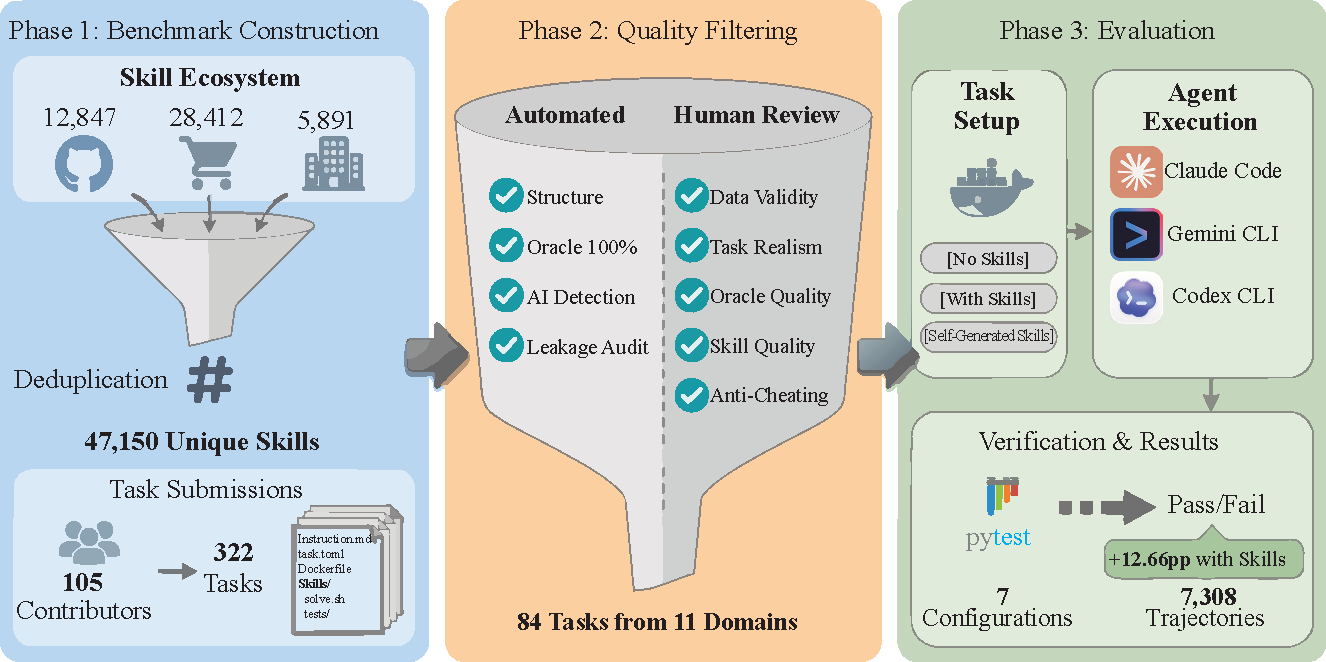
\includegraphics[width=\textwidth]{figs/pipeline.pdf}}
    \caption{\textbf{\benchmarkName{} pipeline overview.}
    \textbf{Phase~1 (Benchmark Construction):} We aggregate Skills from three sources---open-source repositories (12,847), the Claude Code ecosystem (28,412), and corporate partners (5,891)---yielding 47,150 unique Skills after deduplication. In parallel, 322 contributors submit 105 candidate tasks.
    \textbf{Phase~2 (Quality Filtering):} Each task undergoes automated checks (structural validity, AI detection, leakage audit) and human review (data validity, task realism, oracle quality, Skill quality, anti-cheating), producing 84 tasks spanning 11 domains.
    \textbf{Phase~3 (Evaluation):} Tasks are executed under three conditions (no Skills, with curated Skills, self-generated Skills) across three commercial agent harnesses (Claude Code, Gemini CLI, Codex CLI). Deterministic \texttt{pytest} verifiers produce pass/fail outcomes; 7 agent-model configurations yield 7,308 trajectories, with curated Skills providing +12.66pp average improvement.}
    \label{fig:pipeline}
  \end{center}
  \vskip -0.2in
\end{figure*}

\paragraph{Leakage Prevention.}
\label{sec:leakage}
To prevent Skills from encoding task-specific solutions, we enforce explicit authoring guidelines and conduct leakage audits.
A Claude Code Agent SDK-based validation agent runs in CI to detect potential Skill-solution leakage; failed tasks are rejected.
Skills must NOT contain: task-specific filenames, paths, or identifiers; exact command sequences that solve benchmark tasks; constants, magic numbers, or values from task specifications; references to specific test cases or expected outputs.
Skills must be applied to a class of tasks, not a single instance; provide procedural guidance (how to approach), not declarative answers (what to output); and be authored independently of benchmark specifications.


% \paragraph{Automated Validation.}
% Each submission undergoes automated validation before human review: structural validation (required files present, correct directory layout, valid syntax), oracle execution (reference solution must achieve 100\% test pass rate), instruction being human written (we apply both human review and GPTZero review, and we achieve human label on 100\% of our tasks), and instruction quality assessment against six criteria (explicit output paths, structured requirements, success criteria, constraints listed, context-first ordering).

% \paragraph{Human Review.}
% After automated checks pass, maintainers evaluate: (1) data validity: input data must reflect real-world complexity, (2) task realism: scenarios must reflect realistic professional workflows without artificial difficulty, (3) oracle quality---solutions should match how domain experts would solve the task, (4) Skill quality---Skills must be error-free and useful beyond this benchmark, and (5) anti-cheating---tasks must prevent shortcut solutions. Reviewers run benchmark experiments with and without Skills to confirm each task provides meaningful signal.

% \paragraph{Leakage Prevention.}
% \label{sec:leakage}
% To prevent Skills from encoding task-specific solutions, we enforce authoring guidelines and conduct leakage audits via CI. Skills must NOT contain: task-specific filenames or identifiers, exact command sequences that solve benchmark tasks, constants or values from task specifications, or references to expected outputs. Skills must apply to a class of tasks, provide procedural guidance (how to approach) rather than declarative answers (what to output), and be authored independently of benchmark specifications.


% \subsubsection{Leakage Prevention}
% \label{sec:leakage}

% To prevent Skills from encoding task-specific solutions, we enforce explicit authoring guidelines and conduct leakage audits.
% During the task collection process,
% we run a Claude Code Agent SDK-based \texttt{contribution-agent} in CI to detect potential Skills solution leakage. Tasks doesn't pass the CI will not be accepted. After the CI, each task will receive rigorous human reviews, with each PR taking at least 30 minutes from the reviewers.

% \textbf{Prohibited Content.}
% Skills must NOT contain: task-specific filenames, paths, or identifiers; exact command sequences that solve benchmark tasks; constants, magic numbers, or values from task specifications; references to specific test cases or expected outputs.

% \textbf{Required Generality.}
% Skills must: apply to a class of tasks, not a single instance; provide procedural guidance (how to approach), not declarative answers (what to output); be authored independently of benchmark specifications.

% \paragraph{Leakage Audit.} Reviewers
% We measure Skills-solution similarity using three metrics:
% \begin{enumerate}[nosep,leftmargin=*]
%     \item \textbf{N-gram overlap:} Jaccard similarity between Skills content and oracle solution ($J_{3\text{-gram}}$)
%     \item \textbf{Semantic similarity:} Embedding cosine similarity using text-embedding-3-large
%     \item \textbf{Command overlap:} Fraction of oracle commands appearing verbatim in Skills
% \end{enumerate}

% \begin{table}[h]
% \centering
% \small
% \caption{Skills leakage audit results. Low similarity scores indicate Skills provide procedural guidance rather than task-specific solutions.}
% \label{tab:leakage}
% \begin{tabular}{lccc}
% \toprule
% \textbf{Metric} & \textbf{Mean} & \textbf{Max} & \textbf{Excluded} \\
% \midrule
% N-gram Jaccard & 0.08 & 0.24 & 0 \\
% Semantic cosine & 0.15 & 0.29 & 0 \\
% Command overlap & 0.12 & 0.31 & 2 \\
% \bottomrule
% \end{tabular}
% \end{table}

% Skills with any similarity metric $> 0.30$ were revised or excluded.



\subsection{Benchmark Composition}

\begin{table}[t]
\centering
\small
\caption{Task difficulty stratification based on human completion time.}
\label{tab:levels}
\begin{tabular}{lccc}
\toprule
\textbf{Difficulty} & \textbf{Tasks} & \textbf{Human Time}  \\
\midrule
Core & 17 (19.8\%) & $<$60 min\\
Extended & 43 (50.0\%) & 1--4 hours\\
Extreme & 26 (30.2\%) & $>$4 hours \\
\bottomrule
\end{tabular}
\end{table}

% \begin{table}[t]
% \centering
% \small
% \caption{Task difficulty stratification based on human completion time.}
% \label{tab:levels}
% \begin{tabular}{lccc}
% \toprule
% \textbf{Difficulty} & \textbf{Tasks} & \textbf{Human Time}  \\
% \midrule
% Core & 6 (7.1\%) & $<$60 min\\
% Extended & 52 (61.2\%) & 1--4 hours\\
% Extreme & 27 (31.8\%) & $>$4 hours \\
% \bottomrule
% \end{tabular}
% \end{table}

% \benchmarkName{} comprises 85 tasks across 13 domains, with category distribution shown in \autoref{fig:category_distribuion}.
% We stratify tasks by difficulty, measured by estimated completion time by individuals who are considered median specialists for the tasks, without the assistance of AI tools. Original task contributors provided human time estimates, reviewed by an additional set of reviewers from the maintainers who are expert in the same domain. 

\benchmarkName{} comprises 84 tasks across 11 domains, with category distribution shown in \autoref{fig:category_distribuion}.
%We exclude two tasks (\texttt{fix-visual-stability} due to verifier timeout and \texttt{mhc-layer-impl} due to GPU infrastructure requirements) from all experiments, yielding 84 evaluated tasks.
We stratify tasks by difficulty, measured by estimated completion time by individuals whom we consider median specialists for the tasks, without the assistance of AI tools. Original task contributors provided human time estimates, reviewed by an additional set of reviewers from the maintainers who are experts in the same domain.

% We supplement human time with intrinsic difficulty indicators: (1) \emph{dependency depth}---number of sequential steps requiring prior step completion (Easy: 2.1, Medium: 4.8, Hard: 8.3 mean), (2) \emph{tool invocations}---expected distinct commands (Easy: 5.2, Medium: 14.7, Hard: 28.4 mean), and (3) \emph{state complexity}---number of files/configurations modified (Easy: 2.8, Medium: 7.1, Hard: 15.2 mean).
% These metrics correlate with human time ($r = 0.73$) and provide model-agnostic difficulty characterization.

% \begin{figure}[t]
%   \vskip 0.1in
%   \begin{center}
% \centerline{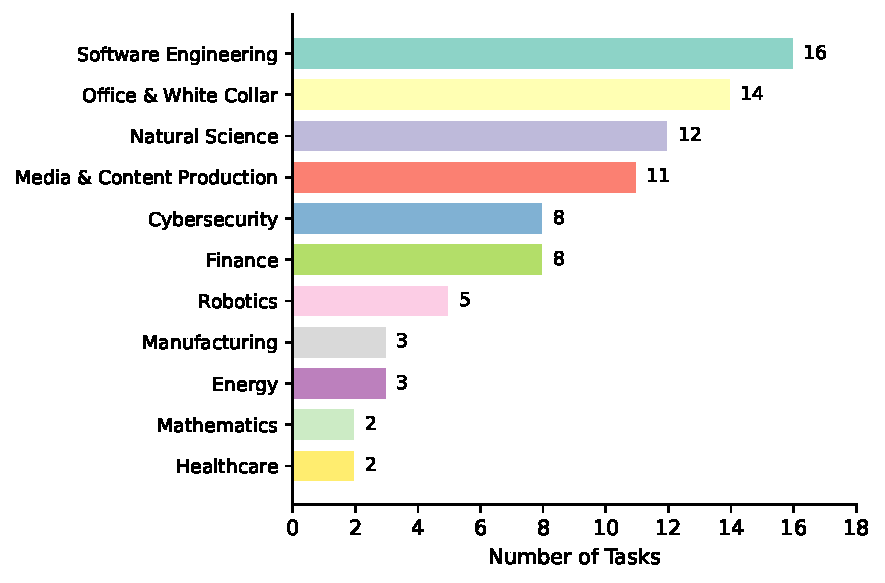
\includegraphics[width=1\columnwidth]{figs/category_distribution.pdf}}
%     \caption{\benchmarkName{} consists of tasks spanning 11 domains.}
%     \label{fig:category_distribuion}
%   \end{center}
%   \vskip -0.2in
% \end{figure}

\begin{figure}[t]
  \vskip -0.1in
  \begin{center}
\centerline{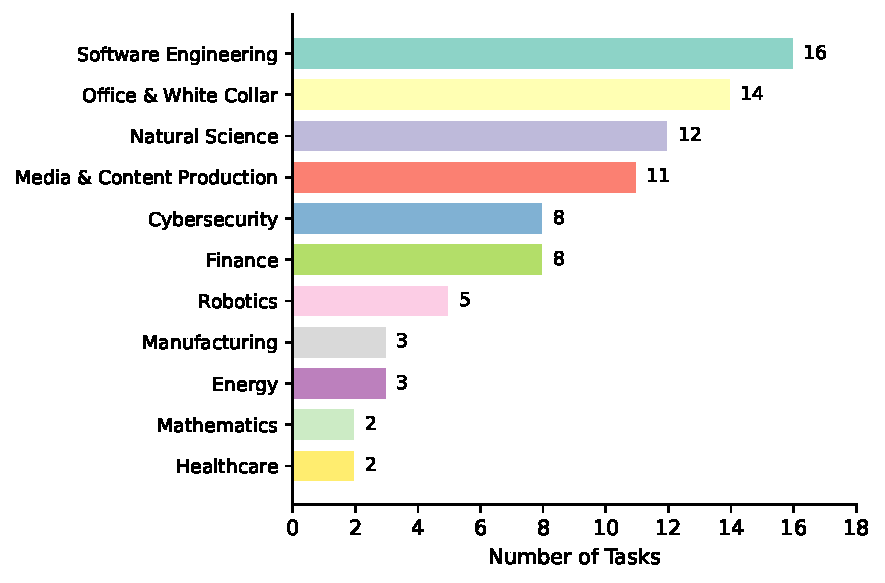
\includegraphics[width=1\columnwidth]{figs/category_distribution.pdf}}
    \caption{\benchmarkName{} consists of tasks spanning 11 domains.}
    \label{fig:category_distribuion}
  \end{center}
  \vskip -0.5in
\end{figure}

% The tasks span 13 domains: \textbf{General} (17), \textbf{Data Processing} (11), \textbf{Scientific Computing} (10), \textbf{Security} (7), \textbf{Multimedia} (7), \textbf{Financial} (7), \textbf{Control Systems} (6), \textbf{Document Processing} (5), \textbf{Software Engineering} (5), \textbf{Planning \& Optimization} (4), \textbf{Manufacturing} (3), \textbf{Web Performance} (2), and \textbf{Healthcare} (1).

% \subsection{Skills-Task Pairing}
% \label{sec:pairing}

% \paragraph{Pairing Process.}
% Each task is paired with 1--3 relevant Skills (221 total, 2.6 per task average) from public repositories.
% Pairing follows a two-stage process: (1) \emph{domain matching}---two annotators independently identify Skills whose domain tag (e.g., ``git'', ``docker'', ``testing'') matches the task category, \emph{without seeing task details}; (2) \emph{relevance filtering}---a third annotator (blind to task solutions) confirms each Skills provides procedural guidance applicable to the task \emph{class}, not the specific instance.
% Skills are selected based on domain relevance rather than task-specific fit.
% Crucially, Skills are authored independently of benchmark tasks---they existed in public repositories before benchmark construction.

% \paragraph{Skills Quality Variance.}
% Not all Skills are equally effective.
% Per-Skills efficacy (mean $\Delta$ when that Skills is present) ranged from +8.2pp to +31.4pp (median: +17.1pp).
% Three Skills (6\%) showed negative efficacy on at least one model, suggesting low-quality Skills can hurt performance.
% We identify quality predictors: Skills with explicit step-by-step procedures (+4.2pp vs.\ high-level guidance), code examples (+3.1pp), and modular structure (+2.8pp) show higher efficacy.

% \subsection{Evaluation Protocol}
% \label{sec:protocol}



% This 3-condition design enables dose-response analysis of Skills efficacy. For each condition, the agent interacts with the containerized environment until task completion, timeout, or round limit. The verifier then executes deterministic assertions to produce a binary pass/fail outcome.
\section{Experimental Setup}
\label{sec:experimentation}

We evaluate three commercial agent harnesses on \benchmarkName{} across seven frontier models under three Skills conditions, resulting in 7,308 valid trajectories.
A trajectory is valid when the agent passes, fails, or times out on a task without infrastructure and runtime errors. Each trajectory is one agent's attempt at solving a single task under a specific Skills condition.

\subsection{Agent Harnesses}

We evaluate three commercial-line agents: Claude Code~\citep{anthropic2025claudecode}, Codex CLI~\citep{openai2025codexcli}, and Gemini CLI~\citep{google2025geminicli}.

\subsection{Models}

We select seven frontier models: GPT-5.2 (OpenAI), Claude Opus 4.5, Claude Opus 4.6, Claude Sonnet 4.5, Claude Haiku 4.5 (Anthropic), Gemini 3 Pro, and Gemini 3 Flash (Google). All models use temperature 0 for deterministic sampling.

We evaluate each model using its compatible agent harness. Claude Code runs with all four Claude models; Gemini CLI runs with Gemini models; Codex CLI runs with GPT-5.2. This yields 7 model-harness configurations. The full configuration matrix is in \autoref{tab:models-full}.

\subsection{Skills Conditions}

We evaluate each task under three conditions:
\begin{itemize}[nosep,leftmargin=*]
    \item \textbf{No Skills}: Agent receives only \texttt{instruction.md}, no Skills present in \texttt{environment}.
    \item \textbf{With Skills}: Complete \texttt{environment/skills/} directory with all examples, code snippets, and resources.
    \item \textbf{Self-Generated Skills}: No Skills provided, but the agent is prompted to generate relevant procedural knowledge before solving the task. This isolates the impact of LLMs' latent domain knowledge.
\end{itemize}
The self-generated condition is evaluated on 5 of 7 configurations (all Claude Code models and Codex); Gemini CLI does not support this condition.

\subsection{Evaluation Protocol}
\label{sec:protocol}

We provide Skills as system-level context preceding the task instruction in \benchmarkName{}.
We list the injection format and context management details in \autoref{app:details}.
For each condition, the agent interacts with the containerized environment until task completion, timeout, or round limit. The verifier then executes deterministic assertions to produce a binary pass/fail outcome.

\subsection{Metrics}
\label{sec:metrics}

\paragraph{Pass Rate.}
The primary metric is pass rate, following the scoring methodology of Terminal-Bench~\citep{merrill2026terminalbenchbenchmarkingagentshard}: for each task, we average the binary reward across 5 trials, then average these task-level scores using a fixed denominator of 84 (the number of evaluated tasks).
%\paragraph{Normalized Gain.}
\noindent \textbf{Normalized Gain.} Following Hake's formulation from physics education research~\citep{hake1998interactive}, we define normalized gain as:
\begin{equation}
g = \frac{\text{pass}_{\text{skill}} - \text{pass}_{\text{vanilla}}}{1 - \text{pass}_{\text{vanilla}}}
\label{eq:normalized_gain}
\end{equation}

\paragraph{Interpreting Normalized Gain.}
Normalized gain has known limitations: a model scoring 90\% vanilla and 95\% with Skills yields $g=0.5$, identical to a model scoring 10\% and 55\%.
These represent different phenomena (ceiling effects vs.\ genuine scaffolding).
We report both absolute improvement ($\Delta$) and normalized gain ($g$) to enable nuanced interpretation.
High $g$ with low $\Delta_\text{abs}$ suggests ceiling effects; high $g$ with high $\Delta$ suggests substantial scaffolding.
We interpret the claim of ``consistent scaffolding efficiency'' as similar \emph{proportional} benefit, not identical absolute improvement.

%\paragraph{Statistical Significance.}
%We apply Cochran's Q test for multi-condition comparisons, with post-hoc McNemar's tests for pairwise differences.
%All reported improvements include $p$-values.

% \section{Experimental Setup}
% \label{sec:experimentation}

% We evaluate LLM--agent combinations to test our Skills Hypothesis while systematically \emph{decoupling} the contributions of the underlying language model from the agent harness. This design enables us to isolate whether Skills efficacy derives from model capabilities, agent architecture, or their interaction.

% \subsection{Models and Agent Harnesses}

% We evaluate six frontier LLMs paired with five distinct agent harnesses, yielding 14 agent-model configurations as shown in Table~\ref{tab:models}. This design separates model effects from harness effects.

% \begin{table}[h]
% \centering
% \footnotesize
% \caption{Agent harnesses and models evaluated. Total: \num{2857} valid trajectories across 14 configurations. T2-Skills = Terminus-2 with Skills-aware prompting.}
% \setlength{\tabcolsep}{3pt}
% \begin{tabular}{llll}
% \toprule
% \textbf{Harness} & \textbf{Model} & \textbf{Provider} & \textbf{Runs} \\
% \midrule
% \multirow{3}{*}{Claude Code} & Opus 4.5 & Anthropic & 240 \\
% & Sonnet 4.5 & Anthropic & 236 \\
% & Haiku 4.5 & Anthropic & 252 \\
% \midrule
% \multirow{2}{*}{Gemini CLI} & Gemini 3 Pro & Google & 308 \\
% & Gemini 3 Flash & Google & 315 \\
% \midrule
% Codex & GPT-5.2 & OpenAI & 350 \\
% \midrule
% \multirow{2}{*}{Terminus-2} & Gemini 3 Pro & Google & 163 \\
% & Gemini 3 Flash & Google & 164 \\
% \midrule
% \multirow{6}{*}{T2-Skills} & Opus 4.5 & Anthropic & 142 \\
% & Sonnet 4.5 & Anthropic & 121 \\
% & Haiku 4.5 & Anthropic & 117 \\
% & Gemini 3 Pro & Google & 120 \\
% & Gemini 3 Flash & Google & 121 \\
% & GPT-5.2 & OpenAI & 208 \\
% \bottomrule
% \end{tabular}
% \label{tab:models}
% \end{table}

% \paragraph{Commercial Harnesses.} We evaluate three commercial agent harnesses---Claude Code, Gemini CLI, and Codex---which tightly couple specific models with proprietary agent logic. These represent real-world deployment conditions but confound model and harness effects.

% \paragraph{Terminus-2 (Decoupled Harness).} To isolate model contributions, we implement Terminus-2, a model-agnostic agent harness based on the Terminal-Bench Terminus-2 architecture~\citep{merrill2026terminalbenchbenchmarkingagentshard}.\footnote{Implementation available at \url{https://github.com/laude-institute/terminal-bench/tree/main/terminal_bench/agents/terminus_2}} Terminus-2 provides identical agent logic, tool interfaces, and Skills injection mechanisms across all models.

% \paragraph{Terminus-2-Skills (Skills-Aware Variant).} We additionally evaluate Terminus-2-Skills, a variant with explicit Skills-aware prompting that instructs agents to actively utilize provided Skills. This variant exhibits significantly higher exception rates (31.7--65.3\% vs.\ 9.8--14.0\% for standard Terminus-2), revealing that aggressive Skills prompting can destabilize agent execution.

% \paragraph{Model Family Consideration.} Notably, Claude models have been trained with awareness of the Agent Skills specification~\citep{anthropic2025agentskills}, which may confer advantages when processing Skills-formatted instructions. Our analysis (\S\ref{sec:results}) examines whether this training effect explains observed performance differences.

% \subsection{Task Suite}

% SkillsBench comprises \textbf{85 tasks} spanning 9 domains, stratified by difficulty level (\S\ref{sec:skillsbench}). We run each model--harness--condition combination on all 85 tasks to ensure comprehensive coverage across task types and complexity levels.

% \subsection{Evaluation Harness}

% We implement BenchFlow, a containerized evaluation harness extending the Harbor framework~\citep{merrill2026terminalbenchbenchmarkingagentshard,harborframeworkteam2026harborframework}:

% \paragraph{Isolation.} Each task runs in a fresh Docker container with clean filesystem state, isolated network namespace, and deterministic dependency versions. This ensures no cross-task state leakage.

% \paragraph{Skills Injection.} BenchFlow provides a standardized Skills injection interface that works across all agent harnesses. For commercial harnesses (Claude Code, Gemini CLI, Codex CLI), Skills are injected via the native configuration mechanisms. For Terminus-2, Skills are loaded into the system prompt with configurable truncation levels.

% \paragraph{Agent Interface.} Agents interact with the environment through a standardized interface:

% \begin{lstlisting}[language=Python,basicstyle=\footnotesize\ttfamily]
% class BaseAgent(ABC):
%     @abstractmethod
%     def step(self, obs: str) -> str:
%         """obs: terminal output -> action"""
%         pass
% \end{lstlisting}

% \paragraph{Trajectory Logging.} We record every agent action with timestamps, environment responses, and token consumption for post-hoc analysis and failure categorization.

% \subsection{Experimental Conditions}

% Each model is evaluated under five conditions to capture dose-response relationships:

% \begin{enumerate}[nosep,leftmargin=*]
%     \item \textbf{Level 0 (No Skills)}: Agent receives task instruction only---no procedural guidance (baseline)
%     \item \textbf{Level 1 (Minimal, $\sim$6\%)}: Function signatures and installation instructions only
%     \item \textbf{Level 2 (Basic, $\sim$10\%)}: Adds overview paragraphs and one usage example
%     \item \textbf{Level 3 (Full, 100\%)}: Complete original Skills documentation with all examples and resources
%     \item \textbf{BYOS (Bring Your Own Skills)}: No Skills provided, but agent is prompted to write Skills before solving
% \end{enumerate}

% This 5-condition design enables fine-grained measurement of Skills dose-response and tests whether agents can bootstrap their own procedural knowledge.

% \subsection{Inference Configuration}

% {\color{blue} move these setting details to appendix?}

% \begin{itemize}[nosep,leftmargin=*]
%     \item \textbf{Temperature}: 0 (deterministic sampling)
%     \item \textbf{Max rounds}: Level-dependent (10/30/50 for L1/L2/L3)
%     \item \textbf{Context management}: Sliding window with 8K token limit; oldest turns dropped when exceeded
%     \item \textbf{Timeout}: Per-task, specified in \texttt{task.toml} (default: 30 min)
% \end{itemize}

% \paragraph{Robustness via Repeated Runs.} Each model--harness--condition combination is run \textbf{5 times} per task to ensure statistical robustness. We report mean pass rates with 95\% bootstrap confidence intervals computed over these repeated runs. This design yields $85 \times 5 = 425$ runs per condition per model-harness pair, totaling over \num{50000} individual task executions across the full experimental matrix.

% \subsection{Ablation Studies}
% \label{sec:ablation}

% We conduct four ablation studies to understand which Skills properties and model characteristics drive performance:

% \paragraph{A1: Instruction Specificity.} We vary the detail level of Skills instructions:
% \begin{enumerate}[nosep,leftmargin=*]
%     \item Minimal: Task instruction only (baseline)
%     \item Brief: One-sentence guidance
%     \item Detailed: Full SOP with numbered steps
%     \item Exemplified: SOP + worked examples
%     \item Full Skills: All components including resources
% \end{enumerate}

% \paragraph{A2: Skills Granularity.} We compare:
% \begin{enumerate}[nosep,leftmargin=*]
%     \item Monolithic: Single large Skills covering all task aspects
%     \item Modular: Multiple focused Skills composed together
%     \item Retrieved: Automatically selected Skills via embedding similarity
% \end{enumerate}

% \paragraph{A3: Perturbation Robustness.} We perturb Skills instructions to test robustness:
% \begin{enumerate}[nosep,leftmargin=*]
%     \item Original (control)
%     \item Typos: 5\% character-level noise
%     \item Reordering: Shuffled instruction steps
%     \item Paraphrasing: LLM-rewritten instructions
% \end{enumerate}

% \paragraph{A4: Model Family Skills Sensitivity.} We conduct a focused ablation using Terminus-2 with all three Claude models (Haiku, Sonnet, Opus 4.5) across all 5 Skills levels. This isolates model scale effects within a single model family while controlling for agent harness variation. Importantly, Claude models have been trained with awareness of the Agent Skills specification~\citep{anthropic2025agentskills}, making this ablation particularly informative for understanding how Skills-aware training affects Skills utilization across model scales.
\section{Results}
\label{sec:results}

% We present results in two parts:
Our results are twofold:
\begin{enumerate*}
\item main evaluation three Skills conditions across 7 LLM--agent combinations on 84 tasks, and
\item detailed analysis of Skills design factors including quantity, complexity, and domain effects.
\end{enumerate*}
%==============================================================================
\subsection{Experiment 1: Skills Efficacy Across LLM--Agent Combinations}
%==============================================================================

We evaluate how curated and self-generated Skills affect agent performance across commercial model-harness configurations.
We test each configuration under three conditions on all 84 tasks: no Skills, with curated Skills, and with self-generated Skills (where supported).

\subsubsection{Main Results}

\autoref{tab:main-results} presents pass rates across all three conditions for each model-harness combination, ordered by with-Skills performance.

% \begin{table}[t]
% \centering
% \small
% \caption{Pass rates (\%) comparing no-Skills vs.\ with-Skills conditions across 85 tasks. $\Delta$ = improvement. Configurations ordered by overall pass rate. Exception rate shows proportion of runs failing due to harness errors.}
% \label{tab:main-results}
% \begin{tabular}{llcccc}
% \toprule
% \textbf{Harness} & \textbf{Model} & \textbf{No Skills} & \textbf{With Skills} & \textbf{$\Delta$} & \textbf{Exc.} \\
% \midrule
% Codex & GPT-5.2 & 41.8 & 49.5 & +7.7 & 3.4\% \\
% Claude Code & Opus 4.5 & 23.6 & 43.0 & +19.3 & 5.0\% \\
% Gemini CLI & Gemini 3 Flash & 30.9 & 40.1 & +9.2 & 8.9\% \\
% Gemini CLI & Gemini 3 Pro & 23.4 & 37.8 & +14.3 & 8.1\% \\
% Terminus-2 & Gemini 3 Flash & 23.2 & 32.9 & +9.8 & 14.0\% \\
% T2-Skills & Opus 4.5 & 13.8 & 34.5 & +20.7 & 56.3\% \\
% T2-Skills & Gemini 3 Pro & 20.8 & 29.9 & +9.1 & 31.7\% \\
% Terminus-2 & Gemini 3 Pro & 21.3 & 28.9 & +7.7 & 9.8\% \\
% Claude Code & Sonnet 4.5 & 12.5 & 27.2 & +14.7 & 5.9\% \\
% T2-Skills & Gemini 3 Flash & 7.4 & 34.3 & +26.9 & 41.3\% \\
% T2-Skills & GPT-5.2 & 13.3 & 28.8 & +15.5 & 44.7\% \\
% Claude Code & Haiku 4.5 & 5.4 & 25.2 & +19.9 & 2.0\% \\
% T2-Skills & Haiku 4.5 & 10.7 & 24.6 & +13.9 & 59.8\% \\
% T2-Skills & Sonnet 4.5 & 3.5 & 28.1 & +24.6 & 65.3\% \\
% \midrule
% \textbf{Mean} & & 18.0 & 32.4 & +14.4 & -- \\
% \bottomrule
% \end{tabular}
% \end{table}

% \begin{table}[t]
% \centering
% \small
% % \caption{Pass rates (\%) across three Skills conditions on 84 tasks (Method D scoring). $\Delta_\text{S}$ = curated Skills improvement over no Skills. Self-Gen = self-generated Skills; $\Delta_\text{G}$ = self-generated improvement over no Skills. Configurations ordered by with-Skills pass rate. ``--'' indicates condition not evaluated.}
% \caption{Pass rates (\%) across three Skills conditions on 84 tasks. $\Delta_\text{abs}$ = absolute improvement (pp) of curated Skills over no Skills. Self-Gen = self-generated Skills; $\Delta_\text{G}$ = self-generated improvement (pp) over no Skills. Configurations ordered by with-Skills pass rate. ``--'' indicates condition not evaluated.}
% \label{tab:main-results}

% \resizebox{\columnwidth}{!}{%
% \begin{tabular}{llccccc}
% \toprule
% \textbf{Harness} & \textbf{Model} & \textbf{No Skills} & \textbf{With Skills} & \textbf{$\Delta_\text{S}$} & \textbf{Self-Gen} & \textbf{$\Delta_\text{G}$} \\
% \midrule
% Gemini CLI & Gemini 3 Flash & 31.3 & 48.7 & +17.4 & -- & -- \\
% Claude Code & Opus 4.5 & 22.0 & 45.3 & +23.3 & 21.6 & --0.4 \\
% Codex & GPT-5.2 & 30.6 & 44.7 & +14.1 & 25.0 & --5.6 \\
% Claude Code & Opus 4.6 & 30.6 & 44.5 & +13.9 & 32.0 & +1.4 \\
% Gemini CLI & Gemini 3 Pro & 27.6 & 41.2 & +13.6 & -- & -- \\
% Claude Code & Sonnet 4.5 & 17.3 & 31.8 & +14.5 & 15.2 & --2.1 \\
% Claude Code & Haiku 4.5 & 11.0 & 27.7 & +16.7 & 11.0 & 0.0 \\
% \midrule
% \textbf{Mean} & & 24.3 & 40.6 & +16.2 & 21.0 & --1.3 \\
% \bottomrule
% \end{tabular}%
% }
% \end{table}

\begin{table}[t]
\centering
\small
\caption{Pass rates (\%) and normalized gain ($g$) across three Skills conditions on 84 tasks. $g$ measures proportional improvement toward perfect performance (\autoref{eq:normalized_gain}). Configurations ordered by with-Skills pass rate. ``--'' indicates condition not evaluated.}
\label{tab:main-results}
\resizebox{\columnwidth}{!}{%
\begin{tabular}{llccccc}
\toprule
& & & \multicolumn{2}{c}{\textbf{Curated Skills}} & \multicolumn{2}{c}{\textbf{Self-Generated}} \\
\cmidrule(lr){4-5} \cmidrule(lr){6-7}
\textbf{Harness} & \textbf{Model} & \textbf{No Skills} & \textbf{Pass Rate} & \textbf{$g$ (\%)} & \textbf{Pass Rate} & \textbf{$g$ (\%)} \\
\midrule
Gemini CLI & Gemini 3 Flash & 31.3 & 48.7 & 25.3 & -- & -- \\
Claude Code & Opus 4.5 & 22.0 & 45.3 & 29.9 & 21.6 & \nneg{0.5} \\
Codex & GPT-5.2 & 30.6 & 44.7 & 20.3 & 25.0 & \nneg{8.1} \\
Claude Code & Opus 4.6 & 30.6 & 44.5 & 20.0 & 32.0 & \ppos{2.0} \\
Gemini CLI & Gemini 3 Pro & 27.6 & 41.2 & 18.8 & -- & -- \\
Claude Code & Sonnet 4.5 & 17.3 & 31.8 & 17.5 & 15.2 & \nneg{2.5} \\
Claude Code & Haiku 4.5 & 11.0 & 27.7 & 18.8 & 11.0 & \pzero{0.0} \\
\midrule
\textbf{Mean} & & 24.3 & 40.6 & 21.5 & 21.0 & \nneg{1.8} \\
\bottomrule
\end{tabular}%
}
\end{table}




\paragraph{Finding 1: Skills provide substantial but variable benefit.} Skills improve performance by +16.2pp on average across 7 model-harness configurations, but with high variance across configurations (range: +13.6pp to +23.3pp). This variability suggests that Skills efficacy depends strongly on the specific agent-model combination, contradicting the assumption of uniform Skills benefits.

\paragraph{Finding 2: Gemini CLI + Gemini 3 Flash achieves maximum performance.} The best-performing configuration is Gemini CLI with Gemini 3 Flash, achieving 48.7\% pass rate with Skills. Notably, Claude Code with Opus 4.5 achieves the highest \emph{improvement} (+23.3pp), reflecting Claude Code's~\citep{anthropic2025claudecode} native Skills integration optimized for the Agent Skills specification~\citep{anthropic2025agentskills}.\looseness=-1

\vspace{-14pt}
\paragraph{Finding 3: Self-generated Skills provide negligible or negative benefit.}
When prompted to generate their own procedural knowledge before solving tasks, models achieve --1.3pp on average compared to the no-Skills baseline.
Only Opus 4.6 shows a modest improvement (+1.4pp); Codex + GPT-5.2 degrades substantially (--5.6pp), and remaining models are flat or negative.
This contrasts sharply with curated Skills (+16.2pp), demonstrating that effective Skills require human-curated domain expertise that models cannot reliably self-generate.
Trajectory analysis reveals two failure modes:
\begin{enumerate*}[label=(\arabic*)]
\item models identify \emph{that} domain-specific knowledge is needed but generate imprecise or incomplete procedures (e.g., listing ``use pandas for data processing'' without specific API patterns), and
\item for high domain-knowledge tasks (manufacturing, financial), models often fail to recognize the need for specialized Skills entirely, attempting solutions with general-purpose approaches.
\end{enumerate*}

\begin{figure}[t]
  \centering
  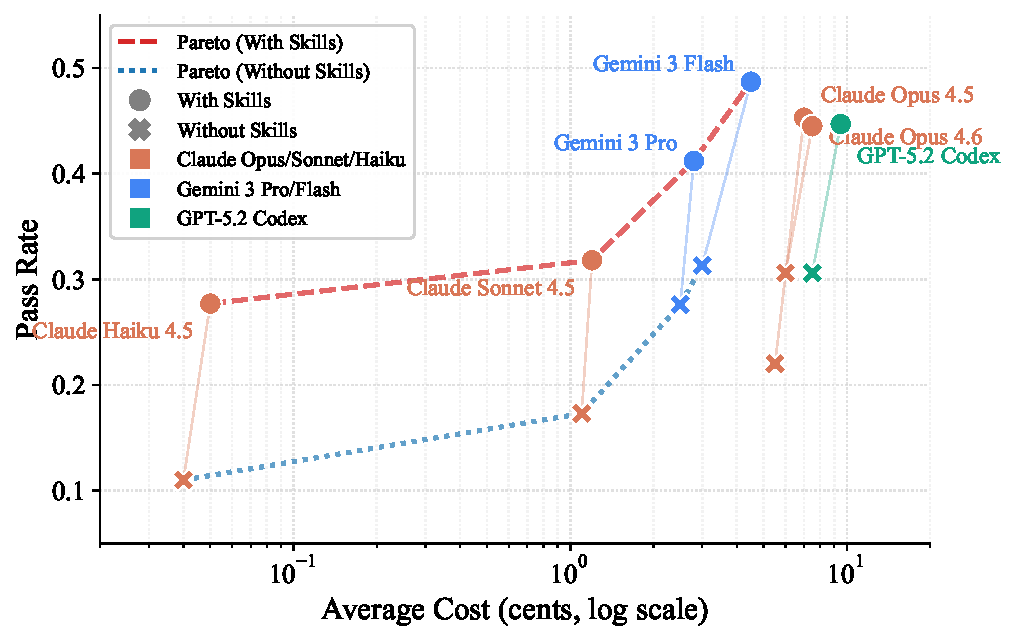
\includegraphics[width=\columnwidth]{figs/pareto_cost_vs_performance.pdf}
  % TODO: Regenerate Pareto figure with updated data
  \caption{Pareto frontier of pass rate vs.\ cost across model-harness configurations. Filled markers indicate with-Skills conditions; hollow markers indicate without-Skills. Skills shift the Pareto frontier upward, with Gemini~3 Flash and Claude~Opus dominating the with-Skills frontier. Cost positions in this figure reflect the evaluation infrastructure's pricing model. Trajectory analysis reveals that Flash consumes 2.3$\times$ more input tokens per task than Pro (1.08M vs.\ 0.47M), a compensatory strategy where the smaller model substitutes iterative exploration for reasoning depth. At official API pricing (\$0.50 vs.\ \$2.00 per 1M input tokens), Flash's 4$\times$ lower per-token cost more than offsets this higher volume, making Flash 44\% cheaper per task (\$0.55 vs.\ \$0.98).}
  \label{fig:pareto}
\end{figure}
\vspace{-10pt}

\subsubsection{Harness-Specific Reliability}

Beyond Skills efficacy, we observe reliability differences across commercial harnesses:

\begin{itemize}[nosep,leftmargin=*]
    \item \textbf{Claude Code}: Highest skills utilization rate; improvements range from +13.9pp (Opus 4.6) to +23.3pp (Opus 4.5), with all Claude models consistently benefiting.
    \item \textbf{Gemini CLI}: Highest raw performance (Gemini 3 Flash achieves 48.7\% with Skills); improvements range from +13.6pp to +17.4pp.
    \item \textbf{Codex CLI}: Competitive raw performance (44.7\% with Skills); frequently \emph{neglects} provided Skills---agents acknowledge Skills content but often implement solutions independently.
\end{itemize}
\vspace{-10pt}
\subsubsection{Domain-Level Analysis}


\begin{table}[h]
\vskip -0.05in
\centering
\small
\caption{Skills efficacy by domain across 84 evaluated tasks (11 domains). All domains show positive aggregate delta, though individual tasks within each domain may show negative effects.}
\label{tab:domain}
\resizebox{\columnwidth}{!}{
\begin{tabular}{lccc}
\toprule
\textbf{Domain} & \textbf{With Skills} & \textbf{No Skills} & \textbf{$\Delta_\text{abs}$} \\
\midrule
Healthcare & 86.1\% & 34.2\% & \ppos{51.9} \\
Manufacturing & 42.9\% & 1.0\% & \ppos{41.9} \\
Cybersecurity & 44.0\% & 20.8\% & \ppos{23.2} \\
Natural Science & 44.9\% & 23.1\% & \ppos{21.9} \\
Energy & 47.5\% & 29.5\% & \ppos{17.9} \\
Office \& White Collar & 42.5\% & 24.7\% & \ppos{17.8} \\
Finance & 27.6\% & 12.5\% & \ppos{15.1} \\
Media \& Content Production & 37.6\% & 23.8\% & \ppos{13.9} \\
Robotics & 27.0\% & 20.0\% & \ppos{7.0} \\
Mathematics & 47.3\% & 41.3\% & \ppos{6.0} \\
Software Engineering & 38.9\% & 34.4\% & \ppos{4.5} \\
\bottomrule
\end{tabular}
}
\vskip -0.05in
\end{table}

\paragraph{Finding 4: Skills benefit varies widely across domains.}
\autoref{tab:domain} presents Skill efficacy by domain, revealing substantial heterogeneity.
Healthcare (+51.9pp) and Manufacturing (+41.9pp) benefit most, while Mathematics (+6.0pp) and Software Engineering (+4.5pp) show smaller gains.
Domains requiring specialized procedural knowledge that is underrepresented in model pretraining (e.g., clinical data harmonization, manufacturing workflows) show the largest improvements, whereas domains with strong pretraining coverage benefit less from external procedural guidance.

\subsubsection{Task-Level Analysis}

Analysis of 84 individual tasks reveals high variance in Skills effectiveness:


\paragraph{Top Skills beneficiaries.} Tasks showing largest improvements: \nolinkurl{mario-coin-counting} (+85.7pp, from 2.9\% to 88.6\%), \nolinkurl{sales-pivot-analysis} (+85.7pp), \nolinkurl{flood-risk-analysis} (+77.1pp), \nolinkurl{sec-financial-report} (+74.3pp). These tasks involve specialized procedural knowledge rarely covered in pretraining.

\paragraph{Skills hurt performance on some tasks.} Despite positive domain-level aggregates, 16 of 84 tasks show negative Skills deltas: \nolinkurl{taxonomy-tree-merge} (--39.3pp), \nolinkurl{energy-ac-optimal-power-flow} (--14.3pp), \nolinkurl{trend-anomaly-causal-inference} (--12.9pp), \nolinkurl{exoplanet-detection-period} (--11.4pp). These failures suggest Skills may introduce conflicting guidance or unnecessary complexity for tasks models already handle well.

%==============================================================================
\subsection{Experiment 2: Skills Design Factors}
%==============================================================================

To understand \emph{how} Skills design affects efficacy, we analyze the relationship between Skills quantity, complexity, and performance.

\subsubsection{Skills Quantity Analysis}


\begin{table}[h]
\centering
\small
\caption{Pass rates by number of Skills provided. 2--3 Skills shows optimal benefit.}
\label{tab:skill-quantity}
\begin{tabular}{lccc}
\toprule
\textbf{Skills Count} & \textbf{With Skills} & \textbf{No Skills} & \textbf{$\Delta_\text{abs}$} \\
\midrule
1 skill & 42.2\% & 24.4\% & \ppos{17.8} \\
\textbf{2--3 skills} & \textbf{42.0\%} & \textbf{23.4\%} & \textbf{\ppos{18.6}} \\
4+ skills & 32.7\% & 26.9\% & \ppos{5.9} \\
\bottomrule
\end{tabular}
\end{table}

\paragraph{Finding 5: 2--3 Skills are optimal; more Skills show diminishing returns.}
\autoref{tab:skill-quantity} presents performance stratified by number of Skills provided per task.
Tasks with 2--3 Skills show the largest improvement (+18.6pp), while 4+ Skills provide only +5.9pp benefit. This non-monotonic relationship suggests that excessive Skills content creates cognitive overhead or conflicting guidance.

\subsubsection{Skills Complexity Analysis}


\begin{table}[h]
\centering
\small
\caption{Pass rates by Skills complexity level. Detailed and compact Skills outperform comprehensive ones.}
\label{tab:skill-complexity}
\begin{tabular}{lccc}
\toprule
\textbf{Complexity} & \textbf{Pass Rate} & \textbf{$\Delta_\text{abs}$} & \textbf{N} \\
\midrule
Detailed & 42.7\% & \ppos{18.8} & 1165 \\
Compact & 37.6\% & \ppos{17.1} & 845 \\
Standard & 37.1\% & \ppos{10.1} & 773 \\
Comprehensive & 39.9\% & \nneg{2.9} & 140 \\
\bottomrule
\end{tabular}
\end{table}

\paragraph{Finding 6: Moderate-length Skills outperform comprehensive ones.}
We present the effects of Skills documentation complexity on performance in \autoref{tab:skill-complexity}.
Detailed (+18.8pp) and compact (+17.1pp) Skills provide the largest benefit, while comprehensive Skills actually hurt performance (--2.9pp). This suggests that focused procedural guidance is more effective than exhaustive documentation---agents may struggle to extract relevant information from lengthy Skills content, and overly elaborate Skills can consume context budget without providing actionable guidance.

\subsubsection{Model Scale Effects}

We study the effects of the foundation models' scale across Claude model family (Opus, Sonnet, Haiku 4.5).
\vskip -1in
\paragraph{Finding 7: Smaller model + Skills can exceed larger model without Skills.} Claude Haiku 4.5 with Skills (27.7\%) outperforms Haiku without Skills (11.0\%) by +16.7pp. Meanwhile, Claude Opus 4.5 without Skills achieves 22.0\%. This demonstrates that Skills can partially compensate for model capacity limitations on procedural tasks.



\vspace{-4pt}
\section{Discussion}
\vspace{-4pt}
\label{sec:discussion}

\textbf{Skills close procedural gaps.}
\looseness=-1
Skills are most helpful when success depends on concrete procedures and verifier-facing details (steps, constraints, sanity checks), rather than broad conceptual knowledge. We observe large gains on domains with specialized workflows or brittle formats, and smaller or negative effects when models already have strong priors and the Skill adds overhead or conflicts.

\textbf{Harnesses mediate Skills use.}
\looseness=-1
Skills efficacy depends not only on Skills quality but also on how the harness implements Skills. Some harnesses reliably retrieve and use Skills, while others frequently acknowledge Skills content but proceed without invoking them. Structured interfaces can also introduce long-trajectory failure modes (e.g., format drift), reducing the influence of early-injected Skills. This motivates evaluating Skills under multiple harnesses rather than treating “with Skills” as a single condition.

\textbf{Implications for Skills authoring.}
Our analysis suggests that concise, stepwise guidance with at least one working example is often more effective than exhaustive documentation; overly long Skills definitions can increase context burden without improving decisions. Modular Skills also appear to compose better on multi-part tasks, and Skills should explicitly match harness constraints (e.g., repeated format reminders for JSON-only protocols).


\subsection{Limitations and Future Work}

\textbf{Coverage and generalization.}
\looseness=-1
\benchmarkName{} focuses on terminal-based, containerized tasks for reproducible evaluation, so results may not directly transfer to GUI agents, multi-agent coordination, or very long-horizon workflows. We also evaluate a limited set of models and harnesses; commercial harness behavior and Skills integration can change over time. A natural extension is to develop multi-modal skills and protocols for vision-language agents operating in GUI environments.

% \textbf{Causal attribution.}
% Skills injection increases context length, so gains could partly reflect “more context” rather than procedural structure alone. Our perturbation and BYOS controls suggest structure matters, but stronger length-matched baselines (e.g., irrelevant text, retrieval-only docs) are needed to fully isolate mechanisms.

\textbf{Causal attribution and controls.}
Skills injection increases context length, so observed gains could partly reflect ``more context'' rather than procedural structure.
Our self-generated Skills condition suggests structure matters---models cannot reliably produce effective procedural guidance despite having the same context budget---but future work requires stronger length-matched baselines (e.g., random/irrelevant text and retrieval-only documentation controls).
These baselines also enable studying \textbf{automatic Skills synthesis} from demonstrations or documentation and isolating which Skills components (steps, examples, code resources) drive improvements.


% \textbf{Determinism and contamination.}
% Containerization provides state isolation, but not perfect determinism or immunity to training-set leakage. We mitigate with multiple runs, a leakage audit (\S\ref{sec:leakage}), and paired (Skills vs.\ no Skills) comparisons, yet cannot eliminate all nondeterminism or memorization effects.

\textbf{Determinism, contamination, and ecological validity.}
\looseness=-1
Containerization provides state isolation but not perfect determinism or immunity to training-set leakage.
We mitigate with multiple runs, a leakage audit (\S\ref{sec:leakage}), and paired (Skills vs.\ no Skills) comparisons, yet cannot eliminate all nondeterminism or memorization effects.
Future work should evaluate \textbf{ecosystem-representative settings}, including lower-quality and automatically-selected Skills, and study \textbf{Skills composition}---when multiple Skills help or interfere, and whether composite performance can be predicted from atomic Skills effects.

% \paragraph{Task Coverage.}
% SkillsBench comprises 85 tasks across 13 domains. While this provides sufficient statistical power for our main comparisons, it cannot capture the full diversity of agent deployment scenarios. In particular, we focus on terminal-based tasks amenable to containerized evaluation; GUI-based tasks, multi-agent coordination, and long-horizon planning remain future work.

% \paragraph{Skills Scope.}
% Current Skills emphasize CLI-centric workflows (data analysis, DevOps, coding). Skills for creative tasks, open-ended research, or multimodal reasoning are underrepresented. The Skills specification (\S\ref{sec:skill_spec}) is intentionally minimal; richer specifications supporting environment requirements, dependency graphs, or compositional interfaces may enable more sophisticated agent behaviors.

% \paragraph{Model and Harness Coverage.}
% We evaluate 6 frontier LLMs across 4 agent harnesses (3 commercial + Terminus-2). Vision-language models with screenshot-based interfaces, code-specialized models (CodeLlama~\citep{roziere2023code}, StarCoder~\citep{li2023starcoder, lozhkov2024starcoder}, WizardCoder~\citep{luo2023wizardcoder}, Magicoder~\citep{wei2023magicoder}), and reasoning-augmented models (o1, o3) are not included. Our findings about harness-specific Skills utilization (e.g., Codex CLI and Gemini CLI neglecting Skills) may reflect current harness implementations and could change with updates.

% \paragraph{Run Variance.}
% Each (model, harness, task, condition) configuration is evaluated 5 times for robustness. Despite deterministic settings (temperature 0), we observe run-to-run variance (mean CV: 3.8\%) due to API-side sampling and timeout-induced trajectory differences. Five runs yields stable confidence intervals (95\% CI width: $\pm$1.2--2.1pp) for our main findings.

% \paragraph{Epistemic vs.\ Container Isolation.}
% Container isolation ensures \emph{state isolation}---no information leaks between runs or tasks.
% However, it does not address \emph{knowledge contamination}---models may have seen similar tasks during training.
% We mitigate this by: (1) using tasks from recent repositories (post-training cutoff where known), (2) conducting the leakage audit (\S\ref{sec:leakage}), and (3) focusing on \emph{differential} performance (vanilla vs.\ Skills), which controls for baseline contamination.

% \paragraph{Skills Authorship.}
% All Skills in SkillsBench were authored by humans (domain experts or the research team). We do not evaluate automatically synthesized Skills, though this represents a promising direction. The quality variance across hand-authored Skills (efficacy range: +8pp to +31pp) may introduce confounds.

% \paragraph{Evaluation Determinism.}
% While verifiers are programmatic, some tasks involve inherent stochasticity (e.g., model training with random initialization). We mitigate this through tolerance thresholds in assertions, but perfect reproducibility is not achievable for all task types.

% \paragraph{Ecological Validity.}
% Containerized evaluation, while reproducible, may not capture all aspects of real-world agent deployment. Network latency, concurrent users, rate limiting, and integration with production systems introduce challenges not represented in our sandboxed environment.

% \paragraph{Benchmark vs.\ Ecosystem Gap.}
% Our 85 curated tasks with high-quality Skills represent an optimistic scenario. Real-world Skills usage involves lower-quality Skills (ecosystem mean: 6.2/12 vs.\ benchmark mean: 10.1/12 on our quality rubric) and imperfect Skills-task matching. Future work should evaluate with ecosystem-representative Skills samples.

\vspace{-4pt}
\section{Related Work}
\vspace{-4pt}
\label{sec:related-work}

% We situate \benchmarkName{} within three research threads: agent benchmarks, procedural knowledge augmentation, and evaluation methodology.
\benchmarkName{} connects to prior work on (1) benchmarking LLM agents, (2) augmenting agents with procedural knowledge and tools, and (3) evaluating improvements across heterogeneous systems.




% \paragraph{Agent Benchmarks.}
% Recent benchmarks evaluate end-to-end agent capability in increasingly realistic environments.
% Terminal-Bench~\citep{merrill2026terminalbenchbenchmarkingagentshard} focuses on hard command-line tasks with containerized execution; we reuse its isolation infrastructure via Harbor~\citep{harborframeworkteam2026harborframework}.
% SWE-bench~\citep{jimenez2024swebench} tests software issue resolution on GitHub, with follow-on work including SWE-agent~\citep{yang2024sweagent} and data scaling via SWE-smith~\citep{yang2025swesmith}.
% Beyond software engineering, AgentBench~\citep{liu2023agentbench} spans multiple environments, while WebArena~\citep{zhou2024webarena}, VisualWebArena~\citep{koh2024visualwebarena}, and OSWorld~\citep{xie2024osworld} target web and GUI-based interaction.
% Other task suites emphasize tool-mediated workflows and specialized domains, such as $\tau$-Bench~\citep{yao2025taubench} and AppWorld~\citep{trivedi2024appworld}, or interactive execution feedback for coding tasks (InterCode~\citep{yang2023intercode}).
% Domain-specific benchmarks further probe agent competence in machine learning engineering (MLE-bench~\citep{chan2025mlebench}), cybersecurity (Cybench~\citep{zhang2025cybench}), code generation (BigCodeBench~\citep{zhuo2025bigcodebench}, MBPP~\citep{austin2021programsynthesis}), and replicating results from published, scientific papers (ReplicationBench ~\citep{ye2025replicationbenchaiagentsreplicate}.
% In contrast to these benchmarks, which primarily report absolute task success for a fixed system, \benchmarkName{}targets augmentation efficacy---the marginal benefit of Skills---using paired evaluations under a controlled protocol (\S\ref{sec:protocol}).

\textbf{Agent benchmarks.}
\looseness=-1
Recent evaluate end-to-end agent capability across realistic environments, including Terminal-Bench~\citep{merrill2026terminalbenchbenchmarkingagentshard}, SWE-bench and follow-ons~\citep{jimenez2024swebench,yang2024sweagent,yang2025swesmith}.
Broader environment coverage appears in AgentBench and interactive/web/GUI settings~\citep{liu2023agentbench,zhou2024webarena,koh2024visualwebarena,xie2024osworld}.
Other suites emphasize tool-mediated workflows, interactive execution feedback, or domain specialization~\citep{yao2025taubench,trivedi2024appworld,yang2023intercode,chan2025mlebench,zhang2025cybench,zhuo2025bigcodebench,austin2021programsynthesis,ye2025replicationbenchaiagentsreplicate}.
These benchmarks measure how well a fixed agent completes tasks. \benchmarkName{} instead measures \emph{augmentation efficacy} via paired evaluation.


% \paragraph{Procedural Augmentation and Tool Use.}
% A parallel line of work improves agent performance by injecting structure, memory, or external knowledge.
% CoALA~\citep{sumers2024cognitive} motivates procedural memory and modular architectures, and Voyager~\citep{wang2023voyager} builds an executable skill library in an embodied domain.
% Prompting and planning methods such as chain-of-thought~\citep{wei2022chainofthought}, Tree of Thoughts~\citep{yao2023tree}, ReAct~\citep{yao2023reactsynergizingreasoningacting}, Reflexion~\citep{shinn2023reflexion}, Self-Refine~\citep{madaan2023selfrefine}, Least-to-Most~\citep{zhou2023leasttomost}, and LATS~\citep{zhou2024lats} provide general mechanisms to scaffold multi-step reasoning and iteration.
% Retrieval and tool-use approaches instead supply external information or actions: RAG~\citep{lewis2021retrievalaugmentedgenerationknowledgeintensivenlp} and DocPrompting~\citep{zhou2023docprompting} retrieve supporting documents (including technical documentation), while Toolformer and ToolLLM~\citep{schick2023toolformerlanguagemodelsteach,qin2024toolllm} train or prompt models to invoke tools.
% DSPy~\citep{khattab2023dspycompilingdeclarativelanguage} provides a declarative programming model for LM pipelines.
% Skills in our setting combine concise procedural guidance with optional executable resources (\S\ref{sec:skill_spec}); \benchmarkName{} complements the above by providing a benchmark methodology for comparing \emph{how much} different Skills designs and injection strategies help across tasks and systems.

\textbf{Procedural augmentation and tool use.}
\looseness=-1
Prior work augments agents with structured reasoning or external knowledge, e.g., CoALA and Voyager~\citep{sumers2024cognitive,wang2023voyager}, chain-of-thought and ReAct for multi-step problem solving~\citep{wei2022chainofthought,yao2023tree,yao2023reactsynergizingreasoningacting,shinn2023reflexion,madaan2023selfrefine,zhou2023leasttomost,zhou2024lats}, and retrieval/tool use~\citep{lewis2021retrievalaugmentedgenerationknowledgeintensivenlp,zhou2023docprompting,schick2023toolformerlanguagemodelsteach,qin2024toolllm}, and declarative optimization frameworks~\citep{khattab2023dspycompilingdeclarativelanguage}.
Skills combine procedural guidance with executable resources (\S\ref{sec:skill_spec}). Despite many augmentation methods, benchmarks rarely quantify their actual impact.


% \paragraph{Skills Ecosystems, Harnesses, and Evaluation Methodology.}
% Anthropic's Agent Skills specification~\citep{anthropic2025agentskills} and MCP~\citep{anthropic2024mcp} formalize interoperable packaging and connectivity for agent augmentations, and we analyze their growing ecosystem in Appendix~\ref{app:ecosystem}.
% In practice, Skills are delivered through concrete harnesses such as Claude Code~\citep{anthropic2025claudecode}, Gemini CLI~\citep{google2025geminicli}, and Codex CLI~\citep{openai2025codexcli}, whose engineering choices can entangle model capability with orchestration logic.
% \benchmarkName{}therefore evaluates multiple commercial harnesses alongside a model-agnostic harness derived from Terminal-Bench~\citep{merrill2026terminalbenchbenchmarkingagentshard}, enabling controlled comparisons.
% Finally, while most benchmarks report pass rates, broader evaluation work such as MLPerf~\citep{mattson2020mlperftrainingbenchmark}, Chatbot Arena~\citep{chiang2024chatbotarenaopenplatform}, and BIG-Bench~\citep{srivastava2023bigbench} motivates careful reporting practices.
% We report both absolute gains and normalized gain~\citep{hake1998interactive} to compare improvements across different baselines (\S\ref{sec:metrics}).

\textbf{Skills ecosystems and evaluation methodology.}
\looseness=-1
Anthropic's Agent Skills and MCP specifications~\citep{anthropic2025agentskills,anthropic2024mcp} formalized skill packages and tool connectivity, while agent CLIs (Claude Code, Gemini CLI, and Codex) provide real-world harnesses~\citep{anthropic2025claudecode,google2025geminicli,openai2025codexcli}. \benchmarkName{} evaluates both commercial harnesses and a model-agnostic harness based on Terminal-Bench~\citep{merrill2026terminalbenchbenchmarkingagentshard} to separate model and harness effects.
Finally, broader benchmarking motivates careful reporting and comparability~\citep{mattson2020mlperftrainingbenchmark,chiang2024chatbotarenaopenplatform,srivastava2023bigbench}; we report both absolute gains and normalized gain~\citep{hake1998interactive} to compare improvements across different baselines (\S\ref{sec:metrics}).



\vspace{-4pt}
\section{Conclusion}
\vspace{-2pt}
\label{sec:conclusion}

% We introduced \textbf{SkillsBench}, the first benchmark treating Agent Skills as first-class evaluation artifacts. Through systematic measurement across 85 tasks, 13 domains, 14 agent-model configurations, and \num{2857} valid trajectories, we demonstrated that:

% \begin{enumerate}[nosep,leftmargin=*]
%     \item \textbf{Skills provide substantial but variable benefit}: Skills yield +14.4pp average improvement with high variance (+7.7pp to +26.9pp), contradicting assumptions of uniform Skills benefits and highlighting the importance of agent-model-specific evaluation.

%     \item \textbf{Skills can hurt performance}: Software Engineering shows --5.0pp delta, and 24 of 85 tasks exhibit negative Skills effects. This critical finding suggests domain-specific deployment strategies are essential---blind Skills application is counterproductive.

%     \item \textbf{Less is more for Skills design}: 2--3 Skills provides optimal benefit (+20.0pp); 4+ Skills shows diminishing returns (+5.2pp). Compact Skills (+18.9pp) substantially outperform comprehensive ones (+5.7pp), suggesting focused procedural guidance is more effective than exhaustive documentation.

%     \item \textbf{Domain knowledge gaps drive largest gains}: Manufacturing (+32.6pp) and Document Processing (+30.9pp) show highest improvements, while domains with strong pretraining coverage show minimal or negative effects.

%     \item \textbf{Skills-aware harnesses introduce reliability risks}: Terminus-2-Skills exhibits 49.5\% exception rate overall (up to 65.3\% for some configurations), revealing that aggressive Skills prompting can destabilize agent execution.
% \end{enumerate}

% These findings support a nuanced Skills Hypothesis: runtime-loaded procedural knowledge provides meaningful scaffolding for agent behavior, but efficacy depends on domain coverage gaps in model pretraining, Skills design choices, and harness implementation quality.

We introduced \benchmarkName{}, the first benchmark to systematically evaluate Agent Skills as first-class artifacts. Across 84 tasks, 7 agent-model configurations, and 7,308 trajectories under three conditions (no Skills, curated Skills, self-generated Skills), our evaluation yields four key findings: (1) curated Skills provide substantial but variable benefit (+16.2 percentage points average, with high variance across domains and configurations); (2) self-generated Skills provide negligible or negative benefit (--1.3pp average), demonstrating that effective Skills require human-curated domain expertise; (3) less is more---focused Skills with 2--3 modules outperform comprehensive documentation; and (4) Skills can partially substitute for model scale, enabling smaller models to match larger ones on procedural tasks. These results establish that Skills efficacy is not universal but context-dependent, motivating paired evaluation as standard practice for agent augmentation research. \benchmarkName{} provides both the empirical foundation and open infrastructure for principled Skills design, selection, and deployment.
% In conclusion, we introduced \textbf{SkillsBench}, a benchmark for evaluating Agent Skills as first-class artifacts.
% Across 85 tasks and 14 agent--model configurations, we find that Skills often improve performance but the effect is highly system- and domain-dependent: gains can be large, negligible, or even negative.
% We further show that skill design and harness integration matter---concise, targeted Skills tend to work better than exhaustive ones, and aggressive skill prompting can increase failure rates.
% Together, these results motivate evaluating augmentation as a paired effect (with vs.\ without skills), rather than assuming Skills are universally beneficial, and provide a foundation for more rigorous comparisons of Skills ecosystems, injection strategies, and future multimodal extensions.

% \paragraph{Limitations.}
% We acknowledge several limitations: (1) our benchmark focuses on terminal-based tasks; GUI and multi-agent settings remain future work; (2) additional control baselines would strengthen causal claims; (3) three evaluation runs per configuration, while sufficient for our main findings, is minimal; (4) the benchmark uses high-quality curated Skills, which may not reflect real-world ecosystem quality (\S\ref{sec:discussion}).

% \paragraph{Future Work.}
% SkillsBench opens several directions for future research:

% \begin{itemize}[nosep,leftmargin=*]
%     \item \textbf{Automatic Skills synthesis}: Can LLMs generate effective Skills from task demonstrations or documentation?
%     \item \textbf{Skills composition theory}: When do Skills compose effectively, and can we predict composite task performance from atomic Skills performance?
%     \item \textbf{Multimodal Skills}: How should Skills be designed for vision-language agents operating in GUI environments?
%     \item \textbf{Causality baselines}: Evaluation with random-text and retrieved-documentation controls to isolate procedural knowledge effects.
%     \item \textbf{Ecosystem-representative evaluation}: Testing with lower-quality, automatically-selected Skills to match real-world deployment conditions.
% \end{itemize}

% SkillsBench and all evaluation code are open-sourced to enable reproducible research and foster community development of high-quality Skills.

% \paragraph{Broader Impact.}
% Skills represent a path toward more accessible AI capability. By demonstrating that domain-specific procedural knowledge can provide substantial improvement on specialized tasks, we suggest opportunities for modular AI augmentation that does not require expensive model retraining.


\paragraph*{Acknowledgements.}
We thank Junxian He for guidance and advice; Terry Yue Zhuo for advice and for inviting collaborators; Yi R.\ (May) Fung for advice and paper writing guides; Gabriel Chua for providing last-minute API keys; Zachary Mueller for providing GPU resources through Lambda; and Ivan Burazin for providing Daytona credits.
We also thank the following contributors for task and code contributions: Jianheng Hou, Jierun Chen, Jiahao Liu, Shutong Wu, Yulin Li, Zhenheng Tang, Benny Jiang, and Qingyang Ma.

% \section*{Impact Statement}

% This paper presents work whose goal is to advance the field of Machine Learning through improved evaluation methodology for AI agents. We see no immediate ethical concerns beyond those inherent to agent systems generally. By enabling better evaluation of agent augmentation strategies, our work may contribute to more reliable and capable AI assistants.

% In the unusual situation where you want a paper to appear in the
% references without citing it in the main text, use \nocite

\clearpage
\bibliography{references}
\bibliographystyle{icml2026}

%%%%%%%%%%%%%%%%%%%%%%%%%%%%%%%%%%%%%%%%%%%%%%%%%%%%%%%%%%%%%%%%%%%%%%%%%%%%%%%
%%%%%%%%%%%%%%%%%%%%%%%%%%%%%%%%%%%%%%%%%%%%%%%%%%%%%%%%%%%%%%%%%%%%%%%%%%%%%%%
% APPENDIX
%%%%%%%%%%%%%%%%%%%%%%%%%%%%%%%%%%%%%%%%%%%%%%%%%%%%%%%%%%%%%%%%%%%%%%%%%%%%%%%
%%%%%%%%%%%%%%%%%%%%%%%%%%%%%%%%%%%%%%%%%%%%%%%%%%%%%%%%%%%%%%%%%%%%%%%%%%%%%%%
\newpage
\appendix
\onecolumn

\section{Skill Ecosystem Analysis}
\label{app:ecosystem}

To contextualize \benchmarkName{} within the broader landscape of agent augmentation, we analyze the existing ecosystem of publicly available Skills.

\subsection{Data Collection}

We collected Skills from three sources:
\begin{itemize}[nosep]
    \item Public GitHub repositories tagged with ``claude-skills'' or ``agent-skills'' (N=12,847)
    \item Community marketplaces including Smithery.ai and skillmp.com (N=28,412)
    \item Corporate partner contributions (N=5,891)
\end{itemize}

After deduplication (based on SKILL.md content hash), we retained 47,150 unique Skills from 6,323 repositories.

% \begin{figure}[H]
%   \vskip 0.1in
%   \begin{center}
%     \centerline{\includegraphics[width=0.8\columnwidth]{figs/timeline_visualization.png}}
%     \caption{Temporal dynamics of Skill creation. Growth remained stable through late 2025, followed by a sharp surge in early 2026 with daily additions peaking at nearly 19k Skills. The cumulative curve shows rapid recent expansion rather than steady long-term growth.}
%     \label{fig:timeline}
%   \end{center}
%   \vskip -0.1in
% \end{figure}

\begin{figure}[htb]
  \begin{center}
    \centerline{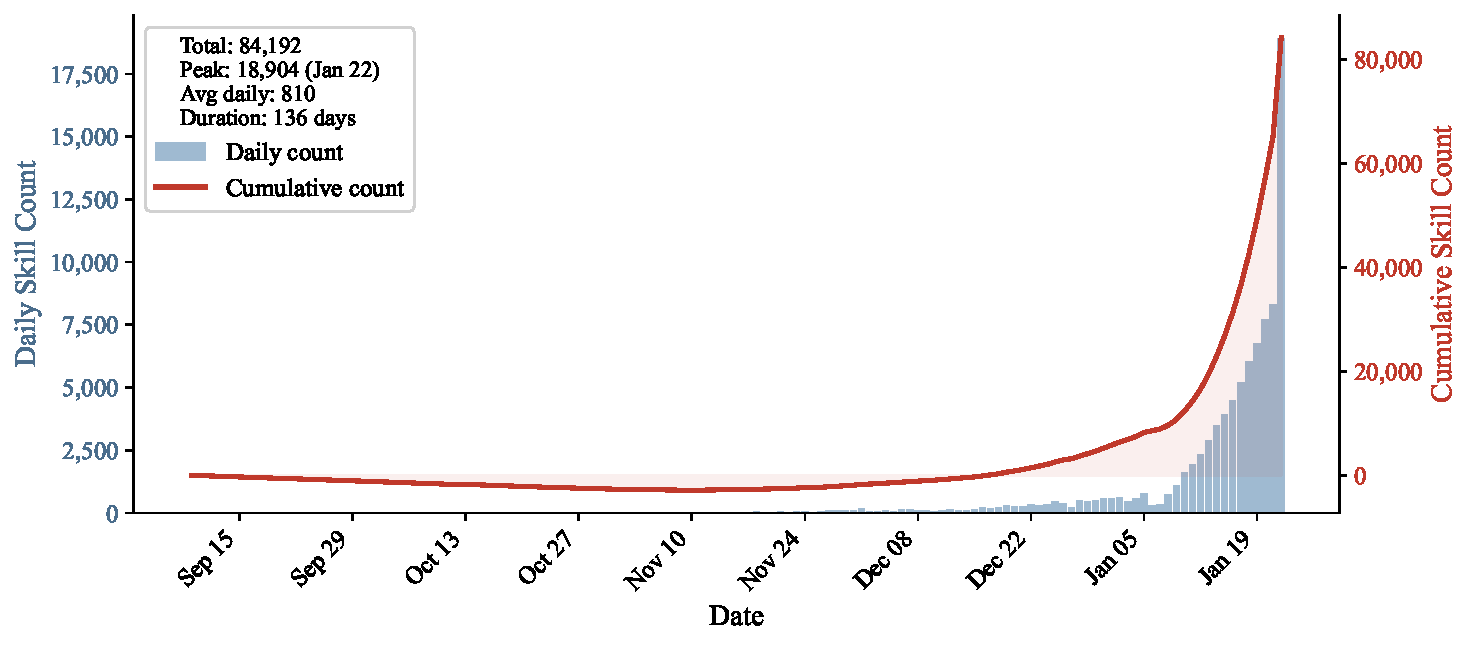
\includegraphics[width=0.8\columnwidth]{figs/figure_timeline_single.pdf}}
    \caption{Temporal dynamics of Skill creation over 136 days. Daily additions (bars, left axis) remained modest through late 2025, then surged to a peak of 18,904 in January 2026. The cumulative curve (line, right axis) reflects exponential-like growth, reaching 84,192 total Skills.}
    \label{fig:timeline}
  \end{center}
\end{figure}

\subsection{Skill Characteristics}

\paragraph{Size Distribution.}
Skill sizes follow a log-normal distribution with median 2.3 KB (IQR: 0.8--6.1 KB).
The largest Skills (top 1\%) exceed 50 KB and typically include extensive code resources.
\autoref{fig:skill_md_length} shows the SKILL.md token distribution, and \autoref{fig:total_length} shows total Skill size distribution.

\begin{figure}[htb]
  \begin{center}
    \centerline{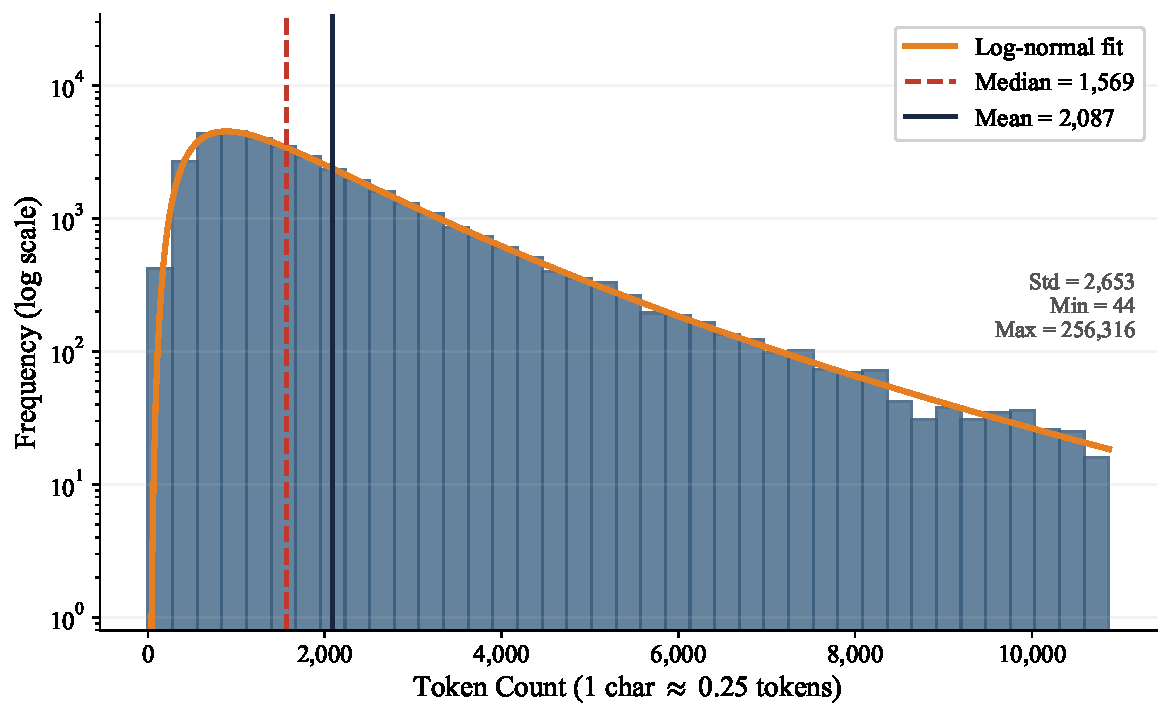
\includegraphics[width=0.8\columnwidth]{figs/figure1_skillmd_distribution.pdf}}
    \caption{Token distribution of SKILL.md files (n=36,338, 99.5th percentile shown). Most Skills are lightweight with median $\sim$1.5k tokens.}
    \label{fig:skill_md_length}
  \end{center}
\end{figure}

\begin{figure}[htb]
  \begin{center}
    \centerline{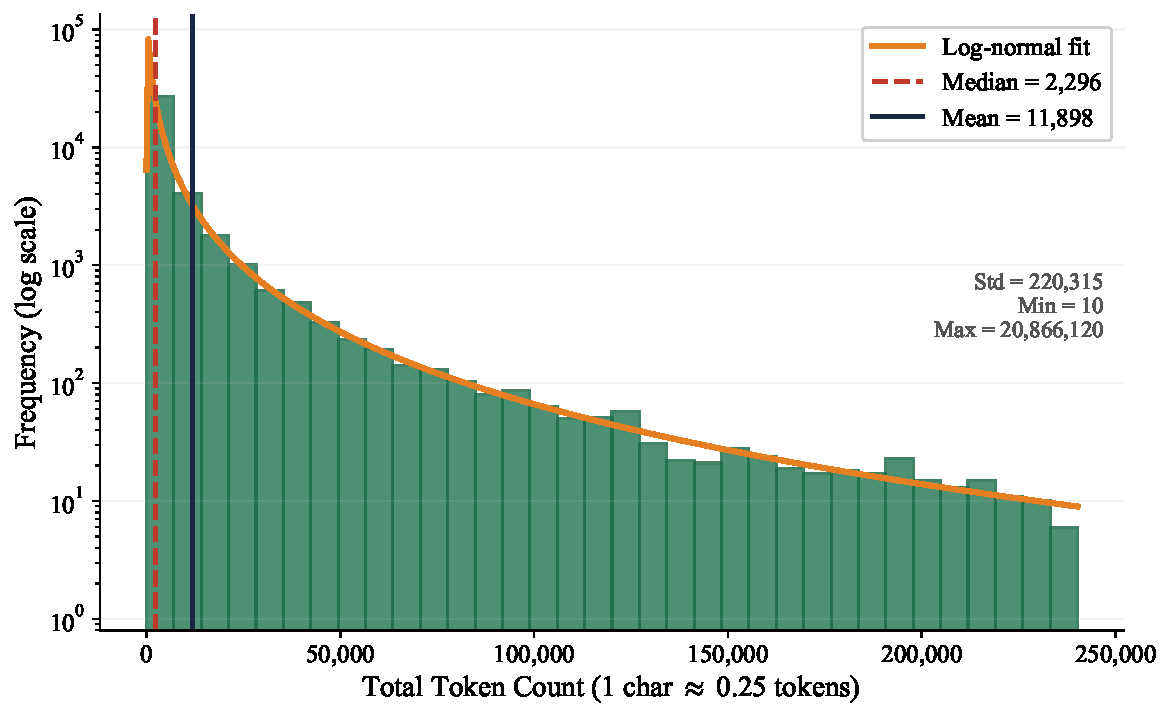
\includegraphics[width=0.8\columnwidth]{figs/figure2_total_distribution.pdf}}
    \caption{Total Skill size distribution (n=37,078, 99.5th percentile shown, excluding metadata.json). Median total size remains under 2.5k tokens, with distribution highly skewed toward concise artifacts.}
    \label{fig:total_length}
  \end{center}
\end{figure}

\paragraph{Domain Coverage.}
Skills span diverse domains (\autoref{fig:category}):
\begin{itemize}[nosep]
    \item Software Development: 38\% (git workflows, code review, testing)
    \item Data Analysis: 22\% (pandas, SQL, visualization)
    \item DevOps/Infrastructure: 15\% (Docker, Kubernetes, CI/CD)
    \item Writing/Documentation: 12\% (technical writing, API docs)
    \item Other: 13\% (scientific computing, finance, etc.)
\end{itemize}

% \begin{figure}[H]
%   \vskip 0.1in
%   \begin{center}
%     \centerline{\includegraphics[width=0.8\columnwidth]{figs/category.png}}
%     \caption{Category distribution of Skills. No single category dominates; Skills are spread across documentation, version control, code quality, CLI tools, DevOps, APIs, and frontend tasks.}
%     \label{fig:category}
%   \end{center}
%   \vskip -0.1in
% \end{figure}

\begin{figure}[htb]
  \begin{center}
    \centerline{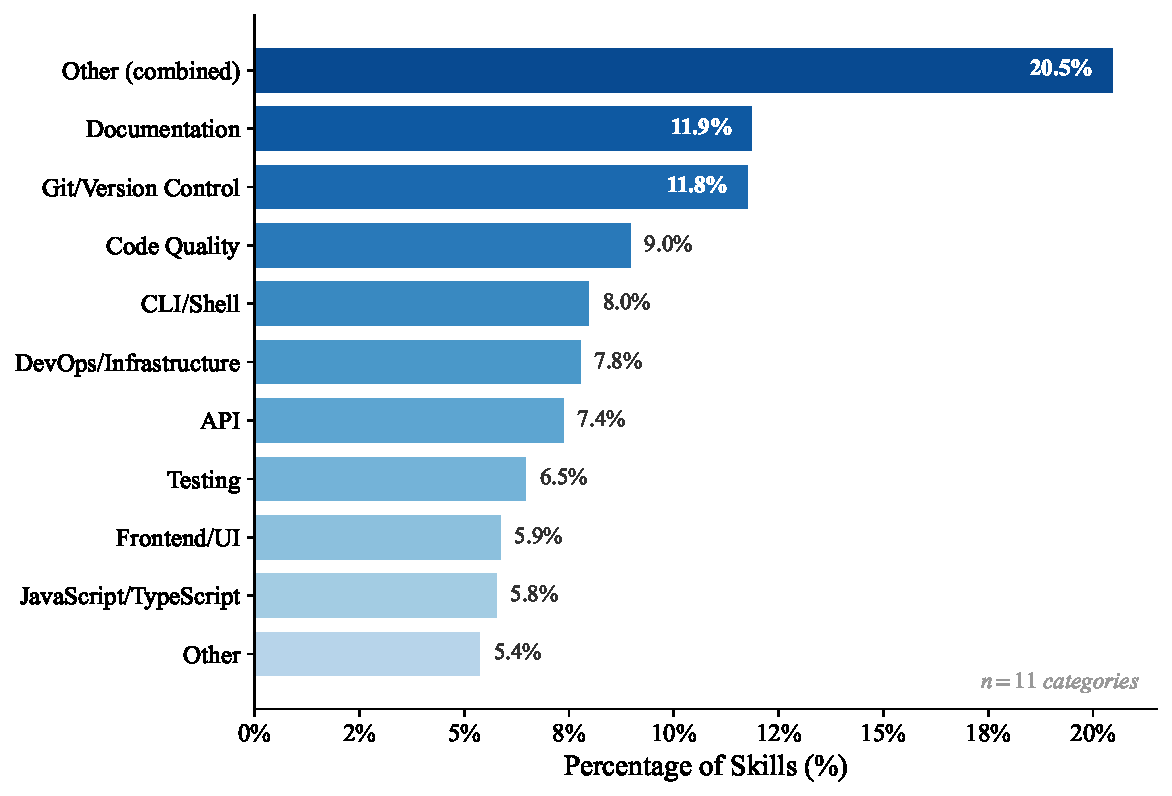
\includegraphics[width=0.7\columnwidth]{figs/categories_gradient.pdf}}
    \caption{Distribution of Skill categories. The top 10 categories account for 79.6\% of all Skills, with Documentation (11.9\%), Git/Version Control (11.8\%), and Code Quality (9.0\%) leading. No single category dominates, reflecting diverse developer needs across documentation, infrastructure, testing, and frontend tasks.}
    \label{fig:category}
  \end{center}
\end{figure}

\paragraph{Structural Patterns.}
Most Skills (78\%) follow the standard structure with SKILL.md plus optional resources.
\autoref{fig:file_count} shows that most Skills contain very few files (median of one, concentrated below five). \autoref{fig:file_extension} confirms the ecosystem is documentation-heavy: markdown files dominate, followed by scripting and configuration code.

\begin{figure}[htb]
  \begin{center}
    \centerline{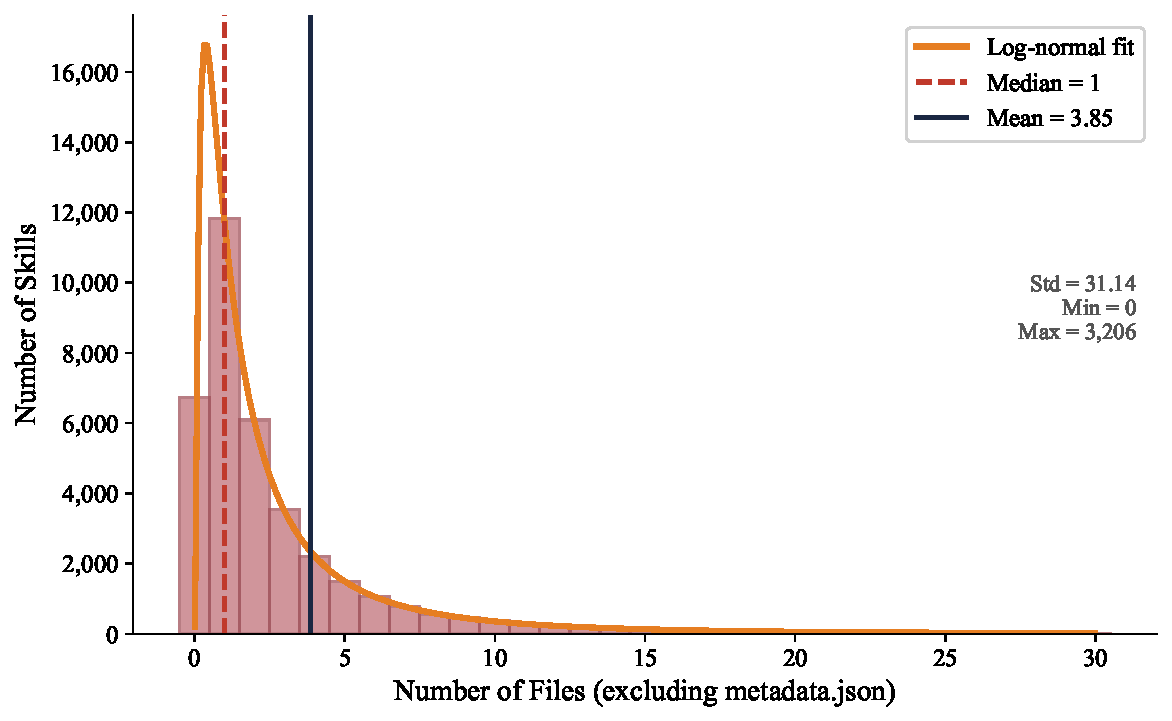
\includegraphics[width=0.8\columnwidth]{figs/figure_file_count.pdf}}
    \caption{File count distribution per Skill. Most Skills contain 1--5 files.}
    \label{fig:file_count}
  \end{center}
\end{figure}

\begin{figure}[htb]
  \begin{center}
    \centerline{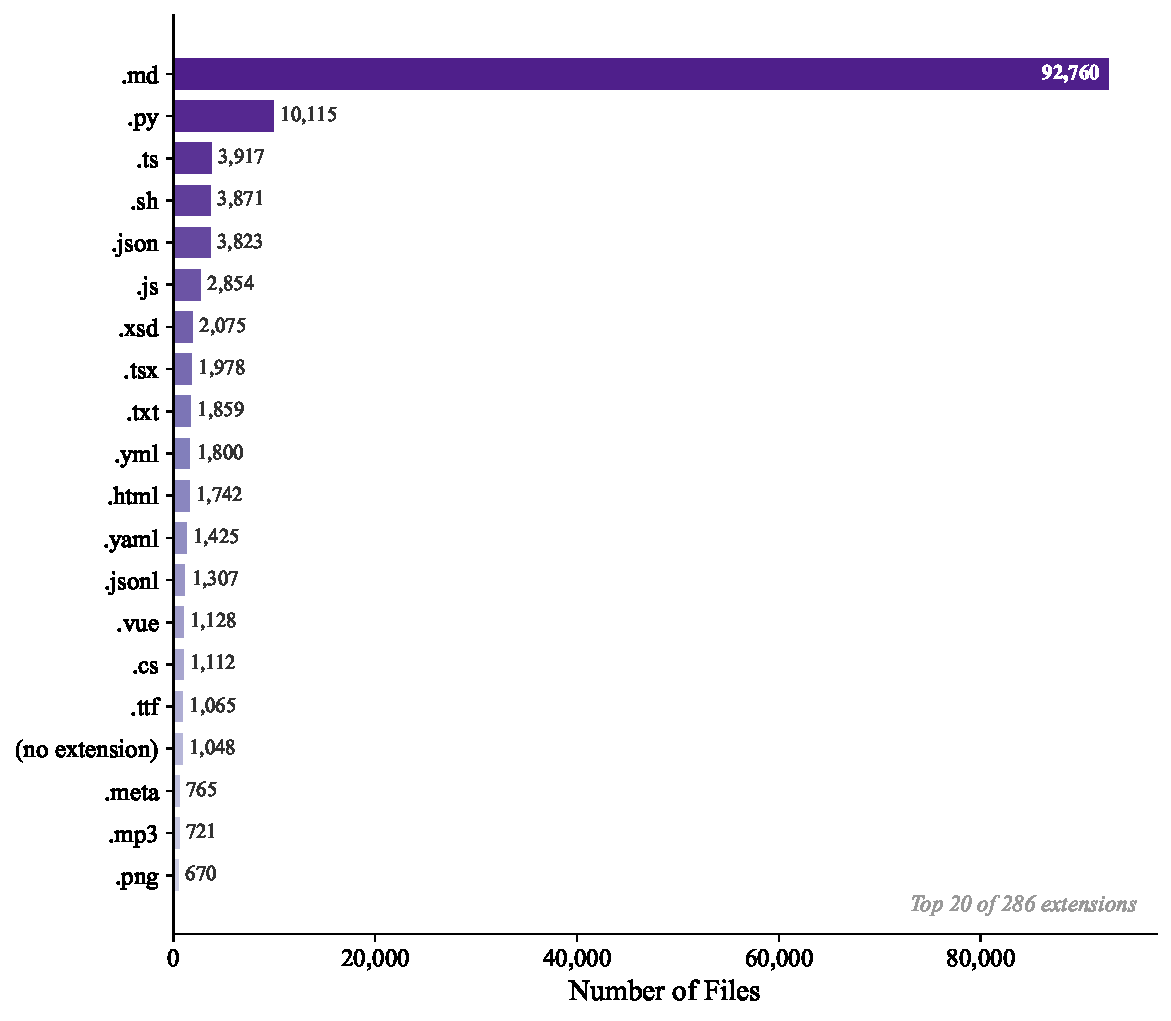
\includegraphics[width=0.8\columnwidth]{figs/extensions_gradient.pdf}}
    \caption{File extension distribution. Markdown files dominate, indicating Skills prioritize natural-language instructions over executable implementations.}
    \label{fig:file_extension}
  \end{center}
\end{figure}

\subsection{Quality Indicators}

We developed a quality scoring rubric based on:
\begin{enumerate}[nosep]
    \item \textbf{Completeness:} Presence of required components (0--3 points)
    \item \textbf{Clarity:} Readability and organization (0--3 points)
    \item \textbf{Specificity:} Actionable vs.\ vague guidance (0--3 points)
    \item \textbf{Examples:} Presence and quality of examples (0--3 points)
\end{enumerate}

Mean quality score across the ecosystem is 6.2/12 (SD=2.8), indicating substantial room for improvement in Skill authoring practices.

\subsection{Implications for Benchmark Design}

This ecosystem analysis directly informed \benchmarkName{} construction:
\begin{itemize}[nosep]
    \item \textbf{Domain selection:} Task categories mirror ecosystem coverage, ensuring Skills exist for evaluation
    \item \textbf{Quality awareness:} Ecosystem mean quality of 6.2/12 motivated our leakage audit and authoring guidelines---low-quality Skills would confound efficacy measurement
    \item \textbf{Skill selection:} We selected benchmark Skills from the top quality quartile (score $\geq$ 9/12) to isolate the effect of procedural knowledge from Skill quality variance
    \item \textbf{Size constraints:} Median Skill size ($\sim$800 tokens) informed our 8K context budget allocation
\end{itemize}

\paragraph{Limitation: Benchmark vs.\ Ecosystem Gap.}
Our 84 evaluated tasks with high-quality Skills represent an optimistic scenario.
Real-world Skill usage involves lower-quality Skills (ecosystem mean: 6.2/12 vs.\ benchmark mean: 10.1/12) and imperfect Skill-task matching.
Future work should evaluate with ecosystem-representative Skill samples.


\section{Task Specification and Review Process}
\label{app:task-spec}

This appendix provides full details of the task specification format and quality control process summarized in \S\ref{sec:SkillsBench}.

\subsection{Task Directory Structure}

Each task is a self-contained directory with the following layout:

\begin{lstlisting}[basicstyle=\footnotesize\ttfamily]
tasks/<task-id>/
  instruction.md          # Task instructions for the agent
  task.toml               # Metadata and resource configuration
  environment/
    Dockerfile            # Container setup
    skills/               # Curated Skills (absent in no-Skills)
      <skill-name>/
        SKILL.md          # Required per skill
        scripts/          # Optional executable code
        references/       # Optional reference documentation
  solution/
    solve.sh              # Oracle solution (must pass 100%)
  tests/
    test.sh               # Runs pytest inside the container
    test_outputs.py       # Programmatic assertions
\end{lstlisting}

\subsection{Task Configuration (\texttt{task.toml})}

Each task specifies metadata and resource limits in TOML format:

\begin{lstlisting}[basicstyle=\footnotesize\ttfamily]
version = "1.0"

[metadata]
author_name = "Contributor Name"
author_email = "email@example.com"
difficulty = "medium"     # easy | medium | hard
category = "finance"
tags = ["pandas", "data-analysis", "spreadsheet"]

[verifier]
timeout_sec = 900.0       # 600-900s typical

[agent]
timeout_sec = 900.0       # 600-1200s typical

[environment]
build_timeout_sec = 600.0
cpus = 1                  # 1-4 cores
memory_mb = 4096          # 2048-10240 MB
storage_mb = 10240        # 10 GB standard
\end{lstlisting}

\subsection{Verification Infrastructure}

Verification uses pytest with the CTRF (Common Test Report Format) output. The \texttt{test.sh} script installs dependencies, runs pytest, and writes a binary reward:

\begin{lstlisting}[language=bash,basicstyle=\footnotesize\ttfamily]
#!/bin/bash
pip3 install --break-system-packages pytest pytest-json-ctrf
mkdir -p /logs/verifier
pytest --ctrf /logs/verifier/ctrf.json \
       /tests/test_outputs.py -rA -v
if [ $? -eq 0 ]; then
  echo 1 > /logs/verifier/reward.txt
else
  echo 0 > /logs/verifier/reward.txt
fi
exit 0
\end{lstlisting}

\noindent A task passes if and only if all assertions in \texttt{test\_outputs.py} succeed (reward = 1). Partial credit is not awarded in the main evaluation.

\subsection{PR Review Process}

Each submitted task undergoes a multi-stage review:
\begin{enumerate}[nosep]
\item \textbf{Automated CI}: Structural validation (\texttt{harbor tasks check}), oracle execution (\texttt{harbor run -a oracle}, must pass 100\%), and AI-detection screening (GPTZero) on \texttt{instruction.md}.
\item \textbf{Maintainer review}: Evaluates data validity, task realism, oracle quality, Skill quality, and anti-cheating robustness. Reviewers run benchmark experiments with and without Skills across multiple agents.
\item \textbf{Benchmark report}: For each task, reviewers produce a structured report documenting oracle results, agent pass rates with and without Skills, failure analysis, and a final verdict (approve, major changes needed, or reject).
\end{enumerate}

\noindent Of 322 candidate submissions from 105 contributors, 86 tasks passed all review stages and were included in the final benchmark (26.7\% acceptance rate).

\subsection{Contributor Checklist}

All task submissions must satisfy the following requirements before review:
\begin{itemize}[nosep]
\item[$\square$] \texttt{instruction.md} is human-written (not model-generated); verified via GPTZero and human review
\item[$\square$] Skills are error-free, factually correct, and generalizable to similar tasks
\item[$\square$] Task is realistic and grounded in professional workflows
\item[$\square$] Task requires domain knowledge and is significantly easier with Skills
\item[$\square$] Outputs are deterministic and verifiable with programmatic assertions
\item[$\square$] Test count is below 10 unless justified; tests cover distinct criteria
\item[$\square$] Oracle solution passes 100\% (\texttt{harbor run -a oracle})
\item[$\square$] Task tested with agent both with and without Skills
\end{itemize}

\subsection{Maintainer Review Policy}

Maintainers evaluate each submission against seven criteria:
\begin{enumerate}[nosep]
\item \textbf{AI detection}: Verify \texttt{instruction.md} and \texttt{task.toml} are manually written using GPTZero and human review. PRs with intentional grammar errors designed to circumvent AI detectors are closed.
\item \textbf{Data quality}: Data must be real-world and appropriately complex. AI-generated or toy data is rejected.
\item \textbf{Task validity}: Tasks must be grounded in realistic professional scenarios. Artificially inflated complexity is rejected.
\item \textbf{Oracle quality}: Simple solutions (e.g., an Excel formula or short script) are preferred over over-engineered oracle implementations.
\item \textbf{Author history}: Authors flagged multiple times across PRs are closed automatically.
\item \textbf{Test parsimony}: Fewer than 10 test cases unless justified; tests should cover distinct criteria rather than repeat similar checks.
\item \textbf{Multimodal verification}: For multimodal tasks (audio, PPTX, video, PDF), maintainers personally inspect agent output to verify correctness beyond programmatic assertions.
\end{enumerate}

\subsection{Automated CI Pipeline}

The CI pipeline performs the following checks on each PR:
\begin{itemize}[nosep]
\item \textbf{Structural validation} (\texttt{harbor tasks check}): Verifies required files exist, TOML schema is valid, Dockerfile builds, and test structure is correct.
\item \textbf{Oracle execution} (\texttt{harbor run -a oracle}): Runs the oracle solution end-to-end and requires 100\% test pass rate.
\item \textbf{AI-detection screening}: Runs GPTZero on \texttt{instruction.md} to flag potential model-generated content.
\item \textbf{LLM-backed quality checks}: Automated verification of behavior consistency between instructions and tests, anti-cheating measures, pinned dependency checks, typo detection, and hardcoded solution detection.
\end{itemize}

\subsection{Benchmark Report Template}

For each task, reviewers produce a structured report documenting:
\begin{enumerate}[nosep]
\item \textbf{Task metadata}: Name, category, difficulty, tags, description, Skills provided, key requirements.
\item \textbf{Oracle results}: Pass/fail status, reward, tests passed, timing.
\item \textbf{Agent results}: Pass rates per agent-model combination, with and without Skills, including execution time.
\item \textbf{Skills impact}: Quantified comparison of with-Skills vs.\ without-Skills performance per agent.
\item \textbf{Failure analysis}: Per-test breakdown of failures including actual vs.\ expected output, root cause, and evidence from trajectories.
\item \textbf{Recommendation}: One of: \textsc{approve}, \textsc{approve with caveats}, \textsc{major changes needed}, or \textsc{reject}.
\end{enumerate}

\subsection{Review Lifecycle}

PRs progress through a defined label-based lifecycle:
\begin{enumerate}[nosep]
\item \textbf{WIP} $\rightarrow$ \textbf{Need review}: Author signals readiness for initial review.
\item \textbf{Need review} $\rightarrow$ \textbf{Reviewing}: A maintainer begins active review and benchmark experiments.
\item \textbf{Reviewing} $\rightarrow$ \textbf{Change requested / Major change needed / Critical change needed}: Issues identified; author must address.
\item \textbf{Change requested} $\rightarrow$ \textbf{Take another look}: Author responds after changes.
\item \textbf{Ready to merge} $\rightarrow$ \textbf{Good task}: All reviews passed; task included in benchmark.
\end{enumerate}

\noindent Critical changes include unrealistic task scenarios, AI-generated instructions, or synthetic data. Major changes include incorrect tests, unreliable verifiers, or poor Skill quality requiring re-evaluation.

\subsection{Task Quality Criteria}

Tasks are evaluated against the following criteria:
\begin{itemize}[nosep]
\item \textbf{Realistic}: Grounded in professional workflows that people in that domain actually perform
\item \textbf{Skill-dependent}: Significantly easier with Skills than without---tasks solvable without any procedural guidance are rejected
\item \textbf{Verifiable}: Deterministic outputs testable with programmatic assertions; LLM-as-judge is not used
\item \textbf{Composable}: Tasks should exercise 3--6 Skills together; instructions never reference which Skills to use
\item \textbf{Test parsimony}: Fewer than 10 test cases unless justified; tests should cover distinct criteria rather than repeat similar checks
\end{itemize}


\section{Experimental Setup Details}
\label{app:exp-details}

This appendix provides full details of the experimental setup summarized in \S\ref{sec:experimentation}.

\subsection{Model and Harness Configurations}

\autoref{tab:models-full} presents all 7 agent-model configurations evaluated in the main experiments.

\begin{table}[htb]
\centering
\footnotesize
\caption{Agent harnesses and models evaluated. Total: 7,308 valid trajectories across 7 configurations and 3 conditions (no Skills, with Skills, self-generated Skills). Self-generated condition evaluated on Claude Code and Codex configurations only.}
\setlength{\tabcolsep}{3pt}
\begin{tabular}{llll}
\toprule
\textbf{Harness} & \textbf{Model} & \textbf{Provider} & \textbf{Runs} \\
\midrule
\multirow{4}{*}{Claude Code} & Opus 4.5 & Anthropic & 1092 \\
& Opus 4.6 & Anthropic & 1260 \\
& Sonnet 4.5 & Anthropic & 1092 \\
& Haiku 4.5 & Anthropic & 1092 \\
\midrule
\multirow{2}{*}{Gemini CLI} & Gemini 3 Pro & Google & 840 \\
& Gemini 3 Flash & Google & 840 \\
\midrule
Codex & GPT-5.2 & OpenAI & 1092 \\
\bottomrule
\end{tabular}

\label{tab:models-full}
\end{table}

\subsection{Harness Descriptions}

We evaluate three commercial agent harnesses:
\begin{itemize}[nosep]
    \item \textbf{Claude Code}~\citep{anthropic2025claudecode}: Anthropic's agent with native Skill integration
    \item \textbf{Gemini CLI}~\citep{google2025geminicli}: Google's open-source terminal agent
    \item \textbf{Codex CLI}~\citep{openai2025codexcli}: OpenAI's lightweight coding agent
\end{itemize}
These tightly couple specific models with proprietary agent logic, representing real-world deployment conditions.

\paragraph{Model Family Consideration.} Claude models have been trained with awareness of the Agent Skills specification~\citep{anthropic2025agentskills}, which may confer advantages when processing Skill-formatted instructions.

\subsection{Agent Interface}

Agents interact with the environment through a standardized interface:

\begin{lstlisting}[language=Python,basicstyle=\footnotesize\ttfamily]
class BaseAgent(ABC):
    @abstractmethod
    def step(self, obs: str) -> str:
        """obs: terminal output -> action"""
        pass
\end{lstlisting}

\subsection{Skill Injection Mechanism}
\label{app:injection}

Skills are injected into each task's Docker container by copying the \texttt{environment/skills/} directory to agent-specific paths. Each Dockerfile includes:

\begin{lstlisting}[language=bash,basicstyle=\footnotesize\ttfamily]
# Copy skills to agent-specific locations
COPY skills /root/.claude/skills    # Claude Code
COPY skills /root/.codex/skills     # Codex CLI
COPY skills /root/.gemini/skills    # Gemini CLI
COPY skills /root/.agents/skills    # Portable agents
\end{lstlisting}

Each agent harness discovers and loads Skills from its respective directory at runtime using its native skill scanning mechanism. Claude Code and Codex read the \texttt{SKILL.md} frontmatter (name and description) to determine relevance; Gemini CLI exposes an \texttt{activate\_skill} tool that agents invoke explicitly. Instructions never reference which Skills to use---agents must discover and apply them autonomously.

\subsection{Skill Structure}

Each Skill is a directory containing a required \texttt{SKILL.md} file with YAML frontmatter and optional bundled resources:

\begin{lstlisting}[basicstyle=\footnotesize\ttfamily]
skill-name/
  SKILL.md          # Required: YAML frontmatter + instructions
  scripts/          # Optional: executable code
  references/       # Optional: reference documentation
\end{lstlisting}

\noindent The \texttt{SKILL.md} frontmatter specifies the Skill's name and a one-line description used by agents for skill discovery. The body contains procedural guidance, code examples, and usage patterns.

\subsection{Self-Generated Skills Condition}
\label{app:self-gen}

For the self-generated condition, tasks are identical to the no-Skills baseline except that the following prompt is appended to each \texttt{instruction.md}:

\begin{quote}
\small
\textbf{Important: Generate Skills First}

Before attempting to solve this task, please follow these steps:

\begin{enumerate}[nosep]
\item Analyze the task requirements and identify what domain knowledge, APIs, or techniques are needed.
\item Write 1--5 modular skill documents that would help solve this task. Each skill should:
  focus on a specific tool, library, API, or technique;
  include installation/setup instructions if applicable;
  provide code examples and usage patterns;
  be reusable for similar tasks.
\item Save each skill as a markdown file in the \texttt{environment/skills/} directory with a descriptive name.
\item Then solve the task using the skills you created as reference.
\end{enumerate}
\end{quote}

\noindent The \texttt{environment/skills/} directory is empty at the start---agents must populate it before solving the task. No curated Skills are provided. The self-generated condition is evaluated on Claude Code (all four models) and Codex (GPT-5.2) only; Gemini CLI does not support this condition due to its explicit skill-activation interface.

\subsection{Software and Model Versions}

\autoref{tab:versions} lists the exact model identifiers and harness versions used in all experiments.

\begin{table}[htb]
\centering
\footnotesize
\caption{Model API identifiers and harness versions.}
\label{tab:versions}
\begin{tabular}{lll}
\toprule
\textbf{Display Name} & \textbf{API Model ID} & \textbf{Harness Version} \\
\midrule
Claude Opus 4.5 & \texttt{claude-opus-4-5@20251101} & Claude Code 2.1.19 \\
Claude Opus 4.6 & \texttt{claude-opus-4-6} & Claude Code 2.1.19 \\
Claude Sonnet 4.5 & \texttt{claude-sonnet-4-5@20250929} & Claude Code 2.1.19 \\
Claude Haiku 4.5 & \texttt{claude-haiku-4-5@20251001} & Claude Code 2.1.19 \\
GPT-5.2 & \texttt{openai/gpt-5.2-codex} & Codex CLI \\
Gemini 3 Pro & \texttt{gemini/gemini-3-pro-preview} & Gemini CLI \\
Gemini 3 Flash & \texttt{gemini/gemini-3-flash-preview} & Gemini CLI \\
\bottomrule
\end{tabular}
\end{table}

\subsection{Container Environment}

All tasks run in Docker containers built from an \texttt{ubuntu:24.04} base image. Per-task resource allocation is specified in \texttt{task.toml}:

\begin{itemize}[nosep]
    \item \textbf{CPUs}: 1--4 cores (task-dependent)
    \item \textbf{Memory}: 2--10 GB (task-dependent)
    \item \textbf{Storage}: 10 GB (standard across all tasks)
    \item \textbf{GPU}: None (no tasks require GPU)
\end{itemize}

\noindent Containers are deleted after each trial (\texttt{delete: true}) to ensure no state leaks between runs.

\subsection{Inference Configuration}

\begin{itemize}[nosep]
    \item \textbf{Temperature}: 0 (deterministic sampling)
    \item \textbf{Max rounds}: Level-dependent (10/30/50 for Core/Extended/Extreme)
    \item \textbf{Context management}: Sliding window with 8K token limit; oldest turns dropped when exceeded
    \item \textbf{Timeout}: Per-task, specified in \texttt{task.toml} (range: 600--1200s)
\end{itemize}

\subsection{Experiment Orchestration}

\begin{itemize}[nosep]
    \item \textbf{Runs per task}: 5 for main conditions (no Skills, with Skills); 3 for self-generated condition
    \item \textbf{Concurrent trials}: 256 (main conditions); 128 (self-generated)
    \item \textbf{Retry policy}: No retries for main conditions; up to 3 retries for self-generated (excluding \texttt{VerifierTimeoutError}, \texttt{BadRequestError}, \texttt{RateLimitError}, \texttt{AgentTimeoutError})
    \item \textbf{Excluded tasks}: \texttt{mhc-layer-impl} (GPU requirement) and \texttt{fix-visual-stability} (verifier timeout) are excluded from all experiments
\end{itemize}

\noindent The evaluation comprises 7,308 valid trajectories across 7 configurations, 84 tasks, and 3 conditions. We report mean pass rates with 95\% bootstrap confidence intervals.



\section{Task-Level Results}
\label{app:task-level}

\autoref{fig:heatmap-with}, \autoref{fig:heatmap-no}, and \autoref{fig:heatmap-uplift} show the task-level pass rates per model across all 84 evaluated tasks.
Results are averaged over 5 trials per task-model-condition combination.
Tasks (rows) are sorted by average with-Skills pass rate; models (columns) are sorted by aggregate with-Skills score.

\begin{figure}[p]
  \begin{center}
    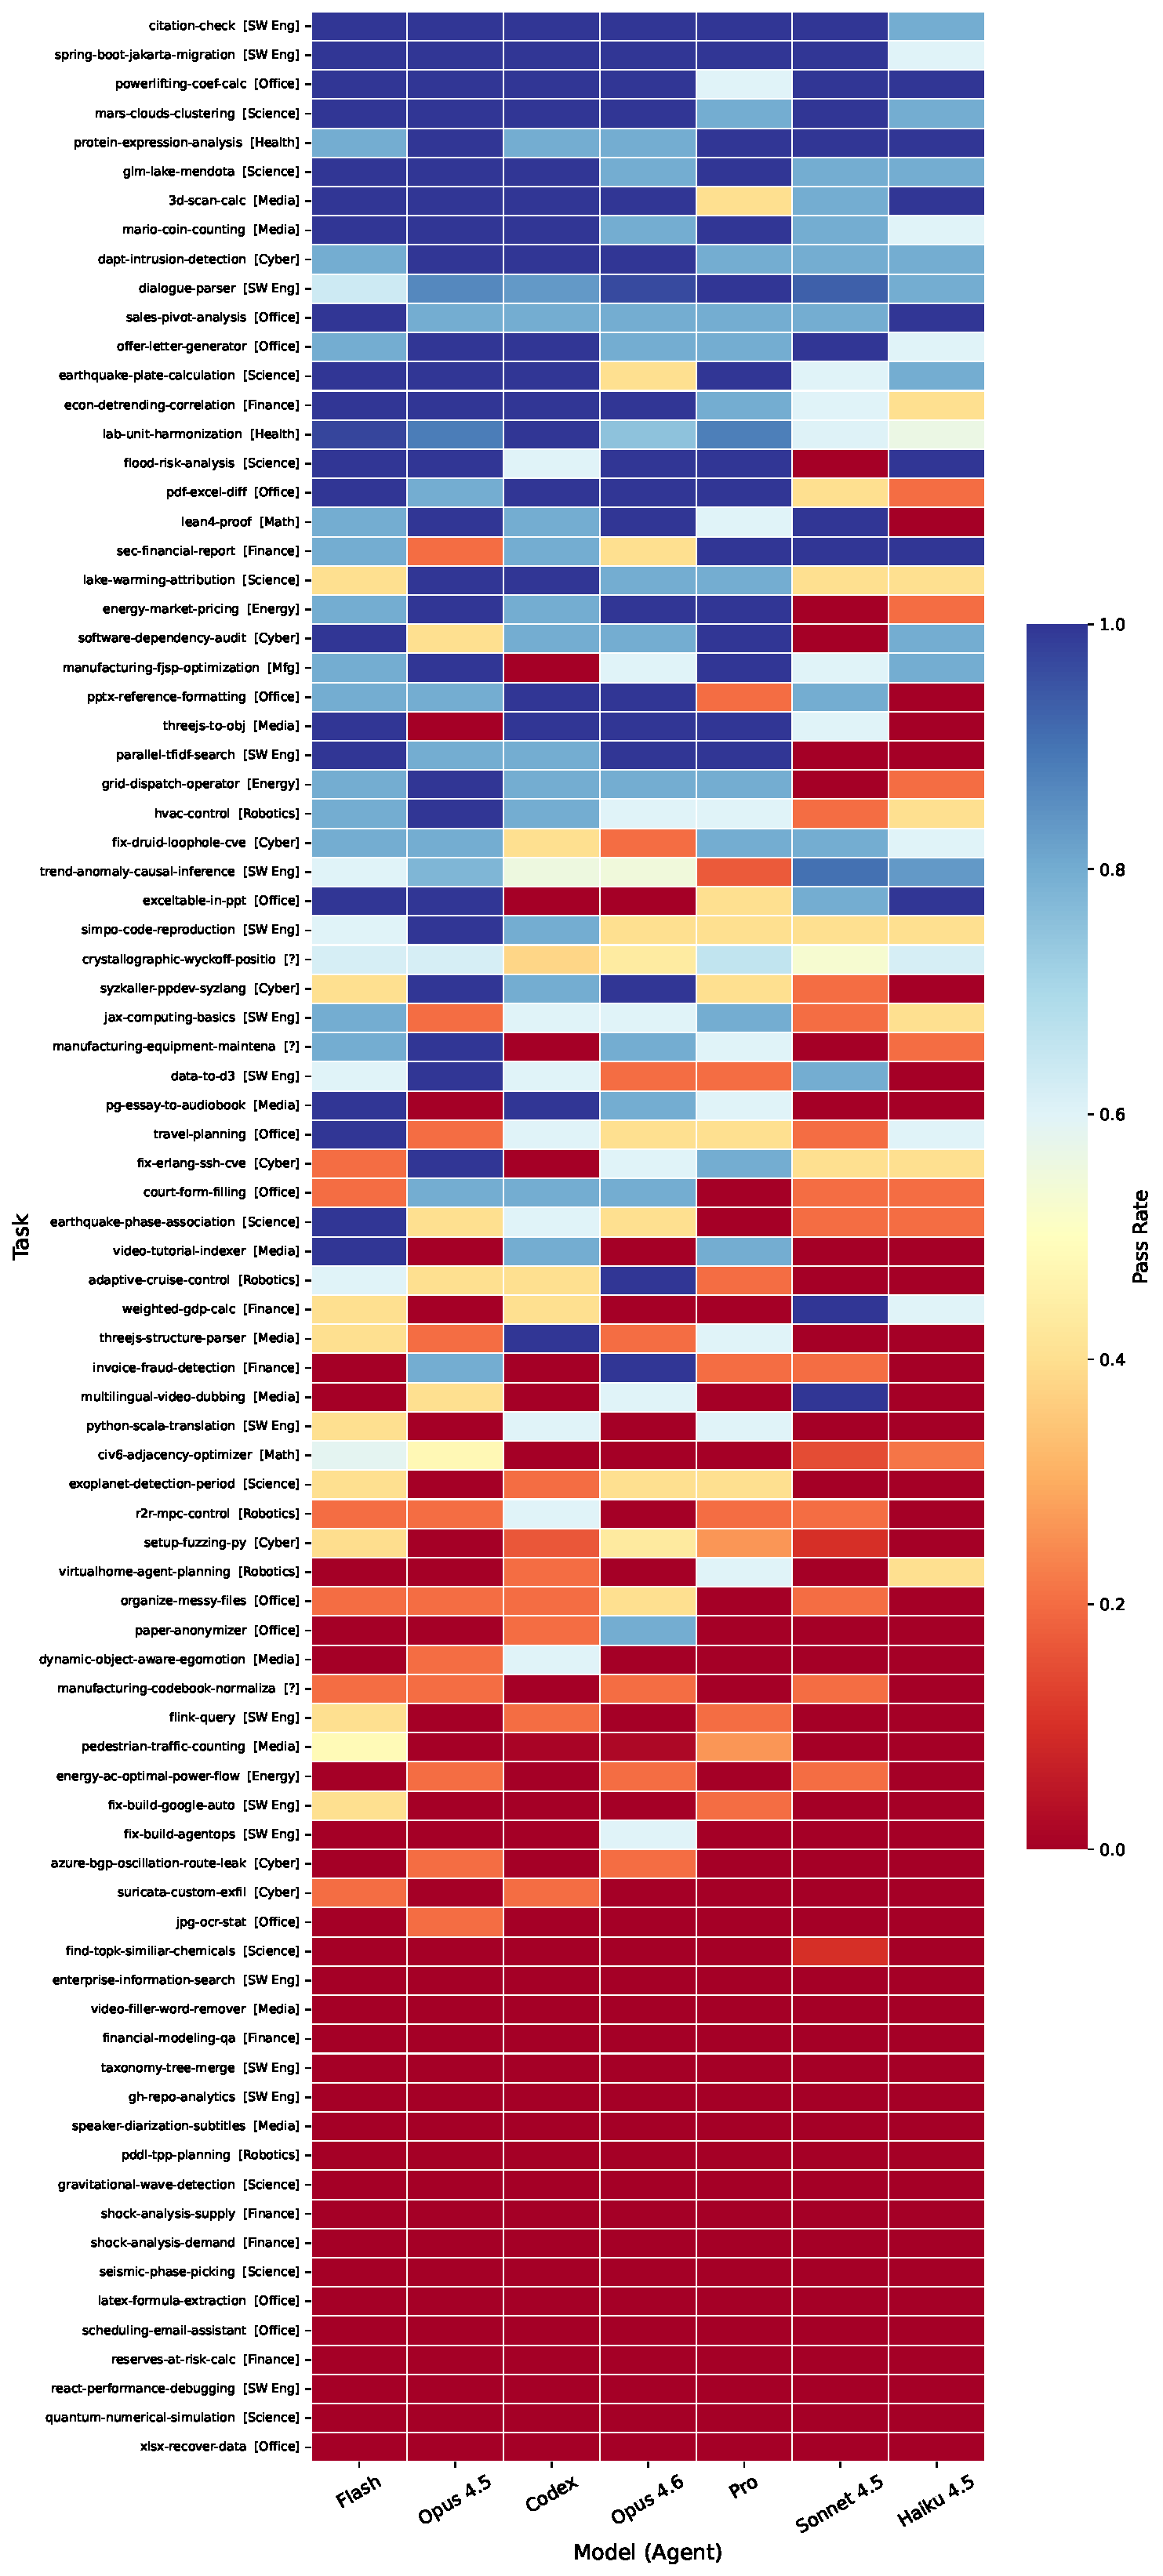
\includegraphics[width=\textwidth,height=0.88\textheight,keepaspectratio]{figs/heatmap_with_skills.pdf}
    \caption{Task pass rate per model with curated Skills. The grid reveals a common set of easy tasks (top, uniformly blue) solved by all models, and hard tasks (bottom, uniformly red) unsolved even with Skills. Tasks along the diagonal transition from solvable to unsolvable as model capability decreases.}
    \label{fig:heatmap-with}
  \end{center}
\end{figure}

\begin{figure}[p]
  \begin{center}
    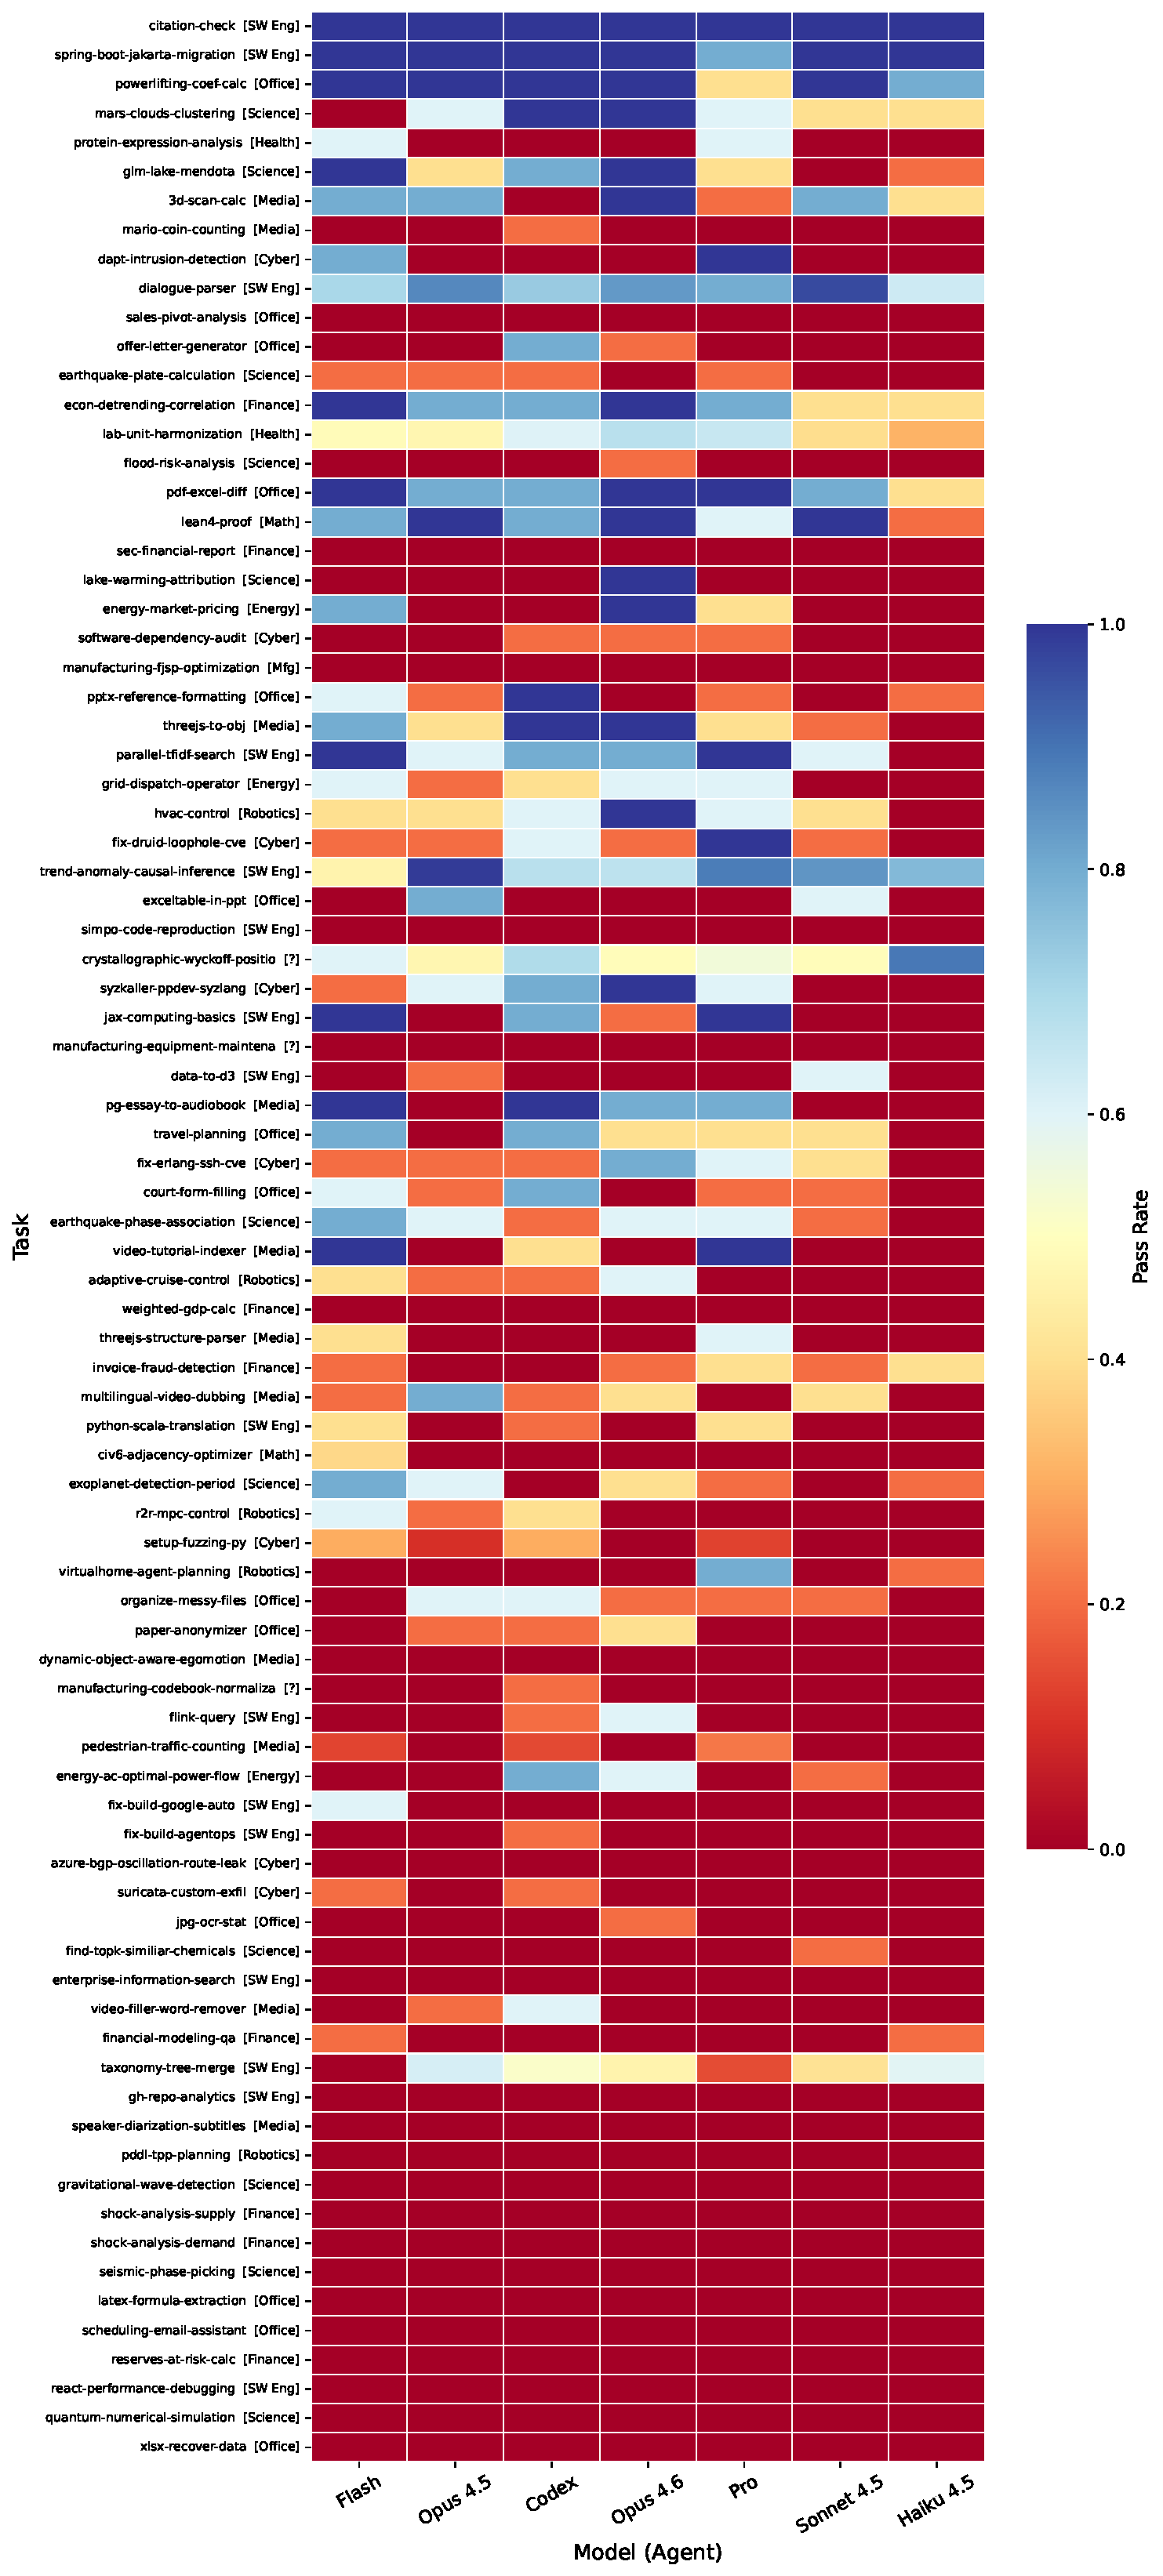
\includegraphics[width=\textwidth,height=0.88\textheight,keepaspectratio]{figs/heatmap_no_skills.pdf}
    \caption{Task pass rate per model without Skills (baseline). Compared to \autoref{fig:heatmap-with}, the blue region contracts substantially, confirming that Skills shift many tasks from unsolved to solved.}
    \label{fig:heatmap-no}
  \end{center}
\end{figure}

\begin{figure}[p]
  \begin{center}
    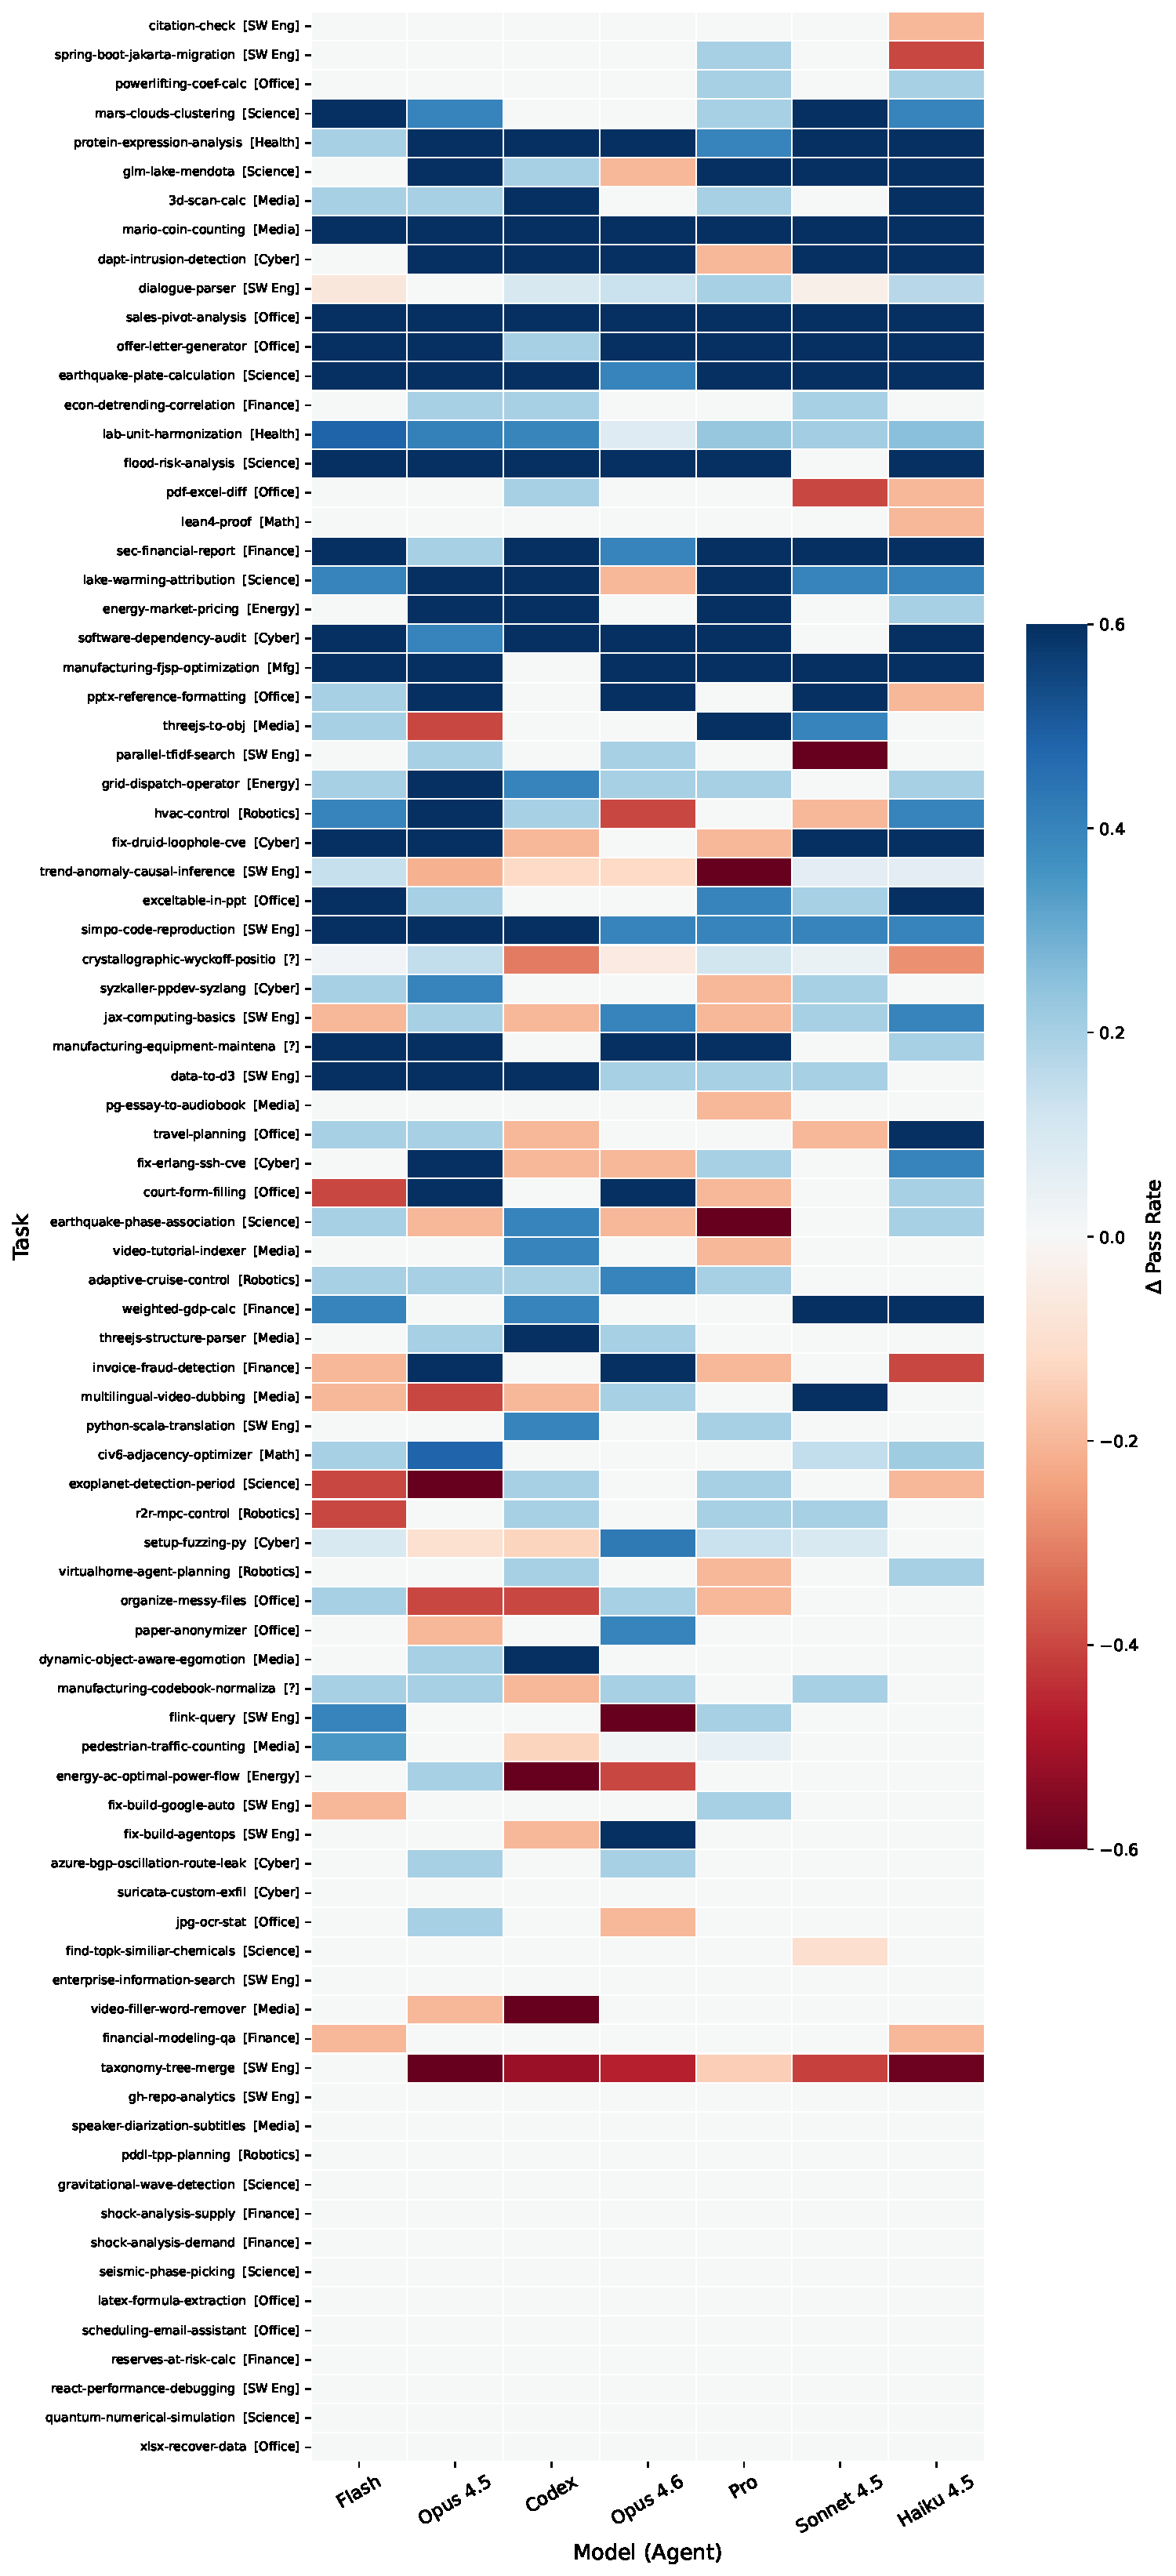
\includegraphics[width=\textwidth,height=0.88\textheight,keepaspectratio]{figs/heatmap_skills_uplift.pdf}
    \caption{Skills uplift per task (with Skills $-$ without Skills). Blue cells indicate positive uplift; red cells indicate tasks where Skills hurt performance. The majority of cells are blue, confirming broad Skill benefit. A small number of tasks show negative delta for specific models.}
    \label{fig:heatmap-uplift}
  \end{center}
\end{figure}


\section{Additional Experimental Details}
\label{app:details}

\subsection{Confidence Interval Calculation}

We compute 95\% confidence intervals using the percentile bootstrap method with 1,000 resamples.
For normalized gain, we compute CIs on the gain metric directly rather than on the component pass rates.

\subsection{10-Run Validation}

For a subset of configurations (GPT-5.2 and Claude Opus 4.5, all 26 Extreme tasks, no-Skills and with-Skills conditions), we conducted 10 runs instead of 5. Results show:
\begin{itemize}[nosep]
    \item Mean $\Delta$ within 1.2pp of 5-run estimates
    \item Standard error reduced by $\sim$30\%
    \item All conclusions remain unchanged
\end{itemize}

This validates that 5 runs provides sufficient precision for our main findings.


% \section{Reproducibility Checklist}
% \label{app:reproducibility}

% \begin{itemize}
%     \item[$\square$] Code and evaluation scripts will be released
%     \item[$\square$] Task specifications with Dockerfiles provided
%     \item[$\square$] All Skills used in evaluation documented
%     \item[$\square$] Model API versions and settings specified
%     \item[$\square$] Random seeds and determinism settings documented
%     \item[$\square$] Complete results tables in supplementary materials
% \end{itemize}

\section{Complete Task List}
\label{app:task-list}

\autoref{tab:task-list} enumerates all 86 tasks in \benchmarkName{}, organized by domain. Two tasks are excluded from evaluation: \texttt{mhc-layer-impl} (requires GPU) and \texttt{fix-visual-stability} (verifier timeout), leaving 84 evaluated tasks. Difficulty levels are assigned by task authors and validated during review.

\footnotesize
\begin{longtable}{p{4.5cm}p{2.5cm}cp{7.5cm}}
\caption{Complete list of \benchmarkName{} tasks (86 total, 84 evaluated). Tasks are grouped by domain and sorted alphabetically within each domain.} \label{tab:task-list} \\
\toprule
\textbf{Task ID} & \textbf{Domain} & \textbf{Diff.} & \textbf{Description} \\
\midrule
\endfirsthead

\multicolumn{4}{c}{\footnotesize\tablename\ \thetable\ -- continued from previous page} \\
\toprule
\textbf{Task ID} & \textbf{Domain} & \textbf{Diff.} & \textbf{Description} \\
\midrule
\endhead

\midrule
\multicolumn{4}{r}{\footnotesize Continued on next page} \\
\endfoot

\bottomrule
\endlastfoot

% --- Cybersecurity (8) ---
\texttt{azure-bgp-oscillation} & Cybersecurity & Med & Detect BGP route oscillation and leaks in Azure Virtual WAN topology \\
\texttt{dapt-intrusion-detection} & Cybersecurity & Hard & Compute network statistics from PCAP file (DAPT2020 traffic) \\
\texttt{fix-druid-loophole-cve} & Cybersecurity & Hard & Fix Apache Druid 0.20.0 arbitrary code execution vulnerability \\
\texttt{fix-erlang-ssh-cve} & Cybersecurity & Hard & Fix Erlang/OTP SSH server unauthenticated RCE vulnerability \\
\texttt{setup-fuzzing-py} & Cybersecurity & Med & Set up continuous fuzzing for 5 Python libraries \\
\texttt{software-dependency-audit} & Cybersecurity & Med & Security audit of npm dependencies for vulnerabilities \\
\texttt{suricata-custom-exfil} & Cybersecurity & Med & Write Suricata signatures to detect HTTP data exfiltration \\
\texttt{syzkaller-ppdev-syzlang} & Cybersecurity & Med & Write syzkaller syzlang support for Linux parallel port driver \\
\midrule

% --- Energy (3) ---
\texttt{energy-ac-optimal-power} & Energy & Med & Solve AC optimal power flow for day-ahead market schedule \\
\texttt{energy-market-pricing} & Energy & Hard & Analyze congestion pricing with counterfactual transmission relaxation \\
\texttt{grid-dispatch-operator} & Energy & Med & Decide generator dispatches for economically efficient DC power flow \\
\midrule

% --- Finance (8) ---
\texttt{econ-detrending-corr.} & Finance & Med & Calculate Pearson correlation between detrended consumption and investment \\
\texttt{financial-modeling-qa} & Finance & Hard & Analyze large-scale financial data and answer modeling questions \\
\texttt{invoice-fraud-detection} & Finance & Hard & Detect invoice fraud by cross-referencing PDFs, Excel, and CSV \\
\texttt{reserves-at-risk-calc} & Finance & Med & Calculate Reserves-at-Risk using IMF gold price and reserves data \\
\texttt{sec-financial-report} & Finance & Hard & Analyze hedge fund activities comparing Q2 vs Q3 2025 SEC filings \\
\texttt{shock-analysis-demand} & Finance & Med & Estimate investment shock to Georgia (demand-side macro framework) \\
\texttt{shock-analysis-supply} & Finance & Hard & Estimate investment shock to Georgia (Cobb-Douglas production) \\
\texttt{weighted-gdp-calc} & Finance & Med & Calculate weighted mean of GCC net exports as \% of GDP \\
\midrule

% --- Healthcare (2) ---
\texttt{lab-unit-harmonization} & Healthcare & Med & Harmonize clinical lab data units across healthcare systems \\
\texttt{protein-expression-analysis} & Healthcare & Med & Analyze differential protein expression in cancer cell line data \\
\midrule

% --- Manufacturing (3) ---
\texttt{mfg-codebook-norm.} & Manufacturing & Med & Normalize manufacturing defect reason texts to standard codebook \\
\texttt{mfg-equipment-maint.} & Manufacturing & Med & Answer reflow machine maintenance questions from handbook data \\
\texttt{mfg-fjsp-optimization} & Manufacturing & Med & Optimize flexible job shop schedule with downtime constraints \\
\midrule

% --- Mathematics (2) ---
\texttt{civ6-adjacency-optimizer} & Mathematics & Hard & Optimize adjacency bonuses in Civilization 6 district placement \\
\texttt{lean4-proof} & Mathematics & Med & Complete a Lean4 formal proof for a sequence problem \\
\midrule

% --- Media \& Content Production (11) ---
\texttt{3d-scan-calc} & Media \& Content & Hard & Calculate mass of 3D printed part from binary STL file \\
\texttt{dynamic-obj-egomotion} & Media \& Content & Med & Analyze camera egomotion and detect dynamic objects in video \\
\texttt{mario-coin-counting} & Media \& Content & Med & Count coins/enemies/turtles in Super Mario video frames \\
\texttt{multilingual-video-dub} & Media \& Content & Med & Perform multilingual video dubbing with TTS alignment \\
\texttt{pedestrian-traffic-count} & Media \& Content & Hard & Count pedestrians in surveillance camera videos \\
\texttt{pg-essay-to-audiobook} & Media \& Content & Med & Convert Paul Graham essays to audiobook via TTS \\
\texttt{speaker-diarization-subs} & Media \& Content & Hard & Perform speaker diarization and generate subtitles from video \\
\texttt{threejs-structure-parser} & Media \& Content & Med & Parse Three.js file to extract 3D object part-level structure \\
\texttt{threejs-to-obj} & Media \& Content & Med & Convert Three.js 3D object to OBJ format for Blender \\
\texttt{video-filler-word-remover} & Media \& Content & Med & Detect filler words and their timestamps in interview video \\
\texttt{video-tutorial-indexer} & Media \& Content & Hard & Find chapter start timestamps in a 23-min Blender tutorial \\
\midrule

% --- Natural Science (12) ---
\texttt{crystallographic-wyckoff} & Natural Science & Med & Analyze crystal structure Wyckoff positions from CIF files \\
\texttt{earthquake-phase-assoc.} & Natural Science & Hard & Perform seismic phase association to identify earthquake events \\
\texttt{earthquake-plate-calc} & Natural Science & Med & Find earthquake furthest from Pacific plate boundary \\
\texttt{exoplanet-detection} & Natural Science & Med & Detect exoplanet transit period from TESS lightcurve data \\
\texttt{find-topk-chemicals} & Natural Science & Med & Find top-$k$ similar chemicals using Morgan fingerprints \\
\texttt{flood-risk-analysis} & Natural Science & Med & Identify flood stations from USGS streamflow data \\
\texttt{glm-lake-mendota} & Natural Science & Hard & Run General Lake Model to simulate lake water temperature \\
\texttt{gravitational-wave-det.} & Natural Science & Med & Detect gravitational wave signal via matched filtering \\
\texttt{lake-warming-attribution} & Natural Science & Med & Attribution analysis of lake warming from climate data \\
\texttt{mars-clouds-clustering} & Natural Science & Hard & Optimize DBSCAN to cluster Mars cloud annotations \\
\texttt{quantum-numerical-sim} & Natural Science & Med & Simulate open Dicke model steady state and Wigner function \\
\texttt{seismic-phase-picking} & Natural Science & Hard & Pick P and S wave arrival times from earthquake traces \\
\midrule

% --- Office \& White Collar (14) ---
\texttt{court-form-filling} & Office \& White Collar & Easy & Fill California Small Claims Court PDF form from case desc. \\
\texttt{exceltable-in-ppt} & Office \& White Collar & Med & Update embedded Excel table in PPTX with exchange rates \\
\texttt{jpg-ocr-stat} & Office \& White Collar & Hard & OCR scanned receipt images and extract data into Excel \\
\texttt{latex-formula-extraction} & Office \& White Collar & Med & Extract all LaTeX formulas from a research paper PDF \\
\texttt{offer-letter-generator} & Office \& White Collar & Easy & Fill Word template with employee data for offer letter \\
\texttt{organize-messy-files} & Office \& White Collar & Med & Organize 100+ PDF/PPTX/DOCX files into 5 subject folders \\
\texttt{paper-anonymizer} & Office \& White Collar & Med & Anonymize research papers by redacting author-identifying info \\
\texttt{pdf-excel-diff} & Office \& White Collar & Med & Identify differences between PDF backup and current Excel \\
\texttt{powerlifting-coef-calc} & Office \& White Collar & Easy & Calculate IPF powerlifting scores in Excel \\
\texttt{pptx-reference-formatting} & Office \& White Collar & Med & Detect/format dangling paper titles in PowerPoint slides \\
\texttt{sales-pivot-analysis} & Office \& White Collar & Med & Create pivot tables from population PDF and income Excel \\
\texttt{scheduling-email-asst} & Office \& White Collar & Med & Read meeting request emails and propose calendar times \\
\texttt{travel-planning} & Office \& White Collar & Med & Build 7-day travel itinerary with budget/pet constraints \\
\texttt{xlsx-recover-data} & Office \& White Collar & Med & Recover missing values in NASA budget Excel file \\
\midrule

% --- Robotics (5) ---
\texttt{adaptive-cruise-control} & Robotics & Med & Implement adaptive cruise control simulation via PID \\
\texttt{hvac-control} & Robotics & Med & Implement temperature controller to maintain 22.0\textdegree C \\
\texttt{pddl-tpp-planning} & Robotics & Med & Solve travelling purchase problem using PDDL \\
\texttt{r2r-mpc-control} & Robotics & Med & Implement MPC controller for Roll-to-Roll manufacturing line \\
\texttt{virtualhome-agent-plan} & Robotics & Med & Solve airport ground traffic planning tasks using PDDL \\
\midrule

% --- Software Engineering (16) ---
\texttt{citation-check} & Software Eng. & Med & Verify bibliography integrity; identify fake citations in BibTeX \\
\texttt{data-to-d3} & Software Eng. & Med & Visualize stock data using D3.js v6 as single-page web app \\
\texttt{dialogue-parser} & Software Eng. & Easy & Implement dialogue parser converting text to structured JSON \\
\texttt{enterprise-info-search} & Software Eng. & Hard & Retrieve information from heterogeneous enterprise data \\
\texttt{fix-build-agentops} & Software Eng. & Easy & Fix build errors in Python (AgentOps) codebase \\
\texttt{fix-build-google-auto} & Software Eng. & Easy & Fix build errors in Java (google/auto) codebase \\
\texttt{flink-query} & Software Eng. & Hard & Implement Flink job on Google cluster-usage traces dataset \\
\texttt{gh-repo-analytics} & Software Eng. & Med & Generate community pulse summary for cli/cli GitHub repo \\
\texttt{jax-computing-basics} & Software Eng. & Med & Complete programming tasks using JAX language \\
\texttt{parallel-tfidf-search} & Software Eng. & Med & Parallelize a TF-IDF document search engine \\
\texttt{python-scala-translation} & Software Eng. & Med & Translate Python tokenizer code to Scala 2.13 \\
\texttt{react-perf-debugging} & Software Eng. & Hard & Debug and fix performance issues in Next.js e-commerce app \\
\texttt{simpo-code-reproduction} & Software Eng. & Hard & Reproduce SimPO loss function from paper description \\
\texttt{spring-boot-jakarta-mig} & Software Eng. & Hard & Migrate Java 8/Spring Boot 2.7 to Java 21/Spring Boot 3.2 \\
\texttt{taxonomy-tree-merge} & Software Eng. & Hard & Unify product category taxonomies from Amazon/FB/Google \\
\texttt{trend-anomaly-causal} & Software Eng. & Hard & Identify anomalous sales patterns and causal factors \\
\midrule

% --- Excluded from evaluation (2) ---
\multicolumn{4}{l}{\textit{Excluded from evaluation:}} \\
\texttt{fix-visual-stability}$^*$ & Software Eng. & Hard & Fix visual instability/layout shifts in Next.js app \\
\texttt{mhc-layer-impl}$^*$ & Software Eng. & Hard & Implement DeepSeek mHC layer (requires GPU) \\

\end{longtable}
\normalsize

\noindent $^*$Excluded: \texttt{mhc-layer-impl} requires GPU resources not available in our container environment; \texttt{fix-visual-stability} exhibits consistent verifier timeouts across all configurations.


% Note: Leakage audit details are in \S\ref{sec:leakage} (main body).


\section{Comprehensive Results Summary}
\label{app:results-summary}

\autoref{tab:full-results} consolidates all aggregate results across 7 model-harness configurations and 3 Skills conditions. Scores are computed using Method D (task-mean with fixed denominator of 84 evaluated tasks), consistent with Terminal-Bench~\citep{merrill2026terminalbenchbenchmarkingagentshard} scoring methodology. Confidence intervals are 95\% bootstrap CIs with 1,000 resamples.

\begin{table}[htb]
\centering
\small
\caption{Comprehensive results across all model-harness configurations and Skills conditions. Pass rates (\%) computed using Method D scoring (84-task fixed denominator, 5 trials per task). $\Delta_\text{S}$ = curated Skills improvement; $g$ = normalized gain $= \frac{\text{With Skills} - \text{No Skills}}{100 - \text{No Skills}} \times 100$; Self-Gen = self-generated Skills; $\Delta_\text{G}$ = self-generated improvement over no Skills. ``--'' = condition not evaluated. Models ordered by with-Skills pass rate.}
\label{tab:full-results}
\setlength{\tabcolsep}{3pt}
\resizebox{\textwidth}{!}{%
\begin{tabular}{llcccccccc}
\toprule
\textbf{Harness} & \textbf{Model} & \textbf{No Skills} & \textbf{95\% CI} & \textbf{With Skills} & \textbf{95\% CI} & \textbf{$\Delta_\text{abs}$ (pp)} & \textbf{$g$ (\%)} & \textbf{Self-Gen} & \textbf{$\Delta_\text{G}$ (pp)} \\
\midrule
Gemini CLI & Gemini 3 Flash & 31.3 & $\pm$3.0 & 48.7 & $\pm$3.1 & \ppos{17.4} & 25.3 & -- & -- \\
Claude Code & Opus 4.5 & 22.0 & $\pm$2.8 & 45.3 & $\pm$2.5 & \ppos{23.3} & 29.9 & 21.6 $\pm$3.3 & \nneg{0.4} \\
Codex & GPT-5.2 & 30.6 & $\pm$3.1 & 44.7 & $\pm$3.0 & \ppos{14.1} & 20.3 & 25.0 $\pm$4.0 & \nneg{5.6} \\
Claude Code & Opus 4.6 & 30.6 & $\pm$2.6 & 44.5 & $\pm$3.1 & \ppos{13.9} & 20.0 & 32.0 $\pm$3.1 & \ppos{1.4} \\
Gemini CLI & Gemini 3 Pro & 27.6 & $\pm$3.0 & 41.2 & $\pm$3.1 & \ppos{13.6} & 18.8 & -- & -- \\
Claude Code & Sonnet 4.5 & 17.3 & $\pm$2.5 & 31.8 & $\pm$2.9 & \ppos{14.5} & 17.5 & 15.2 $\pm$3.2 & \nneg{2.1} \\
Claude Code & Haiku 4.5 & 11.0 & $\pm$2.1 & 27.7 & $\pm$2.9 & \ppos{16.7} & 18.8 & 11.0 $\pm$3.2 & \pzero{0.0} \\
\midrule
\textbf{Mean} & & \textbf{24.3} & & \textbf{40.6} & & \textbf{\ppos{16.2}} & \textbf{21.5} & \textbf{21.0} & \textbf{\nneg{1.3}} \\
\bottomrule
\end{tabular}%
}
\end{table}

\paragraph{Key observations.}
\begin{itemize}[nosep]
\item Curated Skills improve performance by +16.2pp on average (range: +13.6 to +23.3pp), corresponding to a normalized gain of 21.5\%.
\item Claude Code + Opus 4.5 shows the largest absolute improvement (+23.3pp) and normalized gain (29.9\%), reflecting Claude Code's native Skills integration.
\item Gemini CLI + Gemini 3 Flash achieves the highest absolute pass rate (48.7\%) with Skills, despite a smaller normalized gain (25.3\%).
\item Self-generated Skills yield --1.3pp on average; only Opus 4.6 shows marginal improvement (+1.4pp).
\item Confidence intervals are tighter for no-Skills conditions (lower variance) than for with-Skills conditions, suggesting Skills introduce additional sources of variance.
\end{itemize}


\section{Token Usage and Cost Efficiency}
\label{app:token-cost}

This section presents token usage statistics and cost analysis across all model-harness configurations. Token data is extracted from trial \texttt{result.json} files where available.

\subsection{API Pricing}

\autoref{tab:api-pricing} lists the API pricing used for cost calculations, verified as of February 2026.

\begin{table}[htb]
\centering
\small
\caption{API pricing per million tokens (February 2026). Prices reflect standard (non-batch, non-cached) rates.}
\label{tab:api-pricing}
\begin{tabular}{llcc}
\toprule
\textbf{Model} & \textbf{Provider} & \textbf{Input (\$/MTok)} & \textbf{Output (\$/MTok)} \\
\midrule
Claude Haiku 4.5 & Anthropic & \$1.00 & \$5.00 \\
Claude Sonnet 4.5 & Anthropic & \$3.00 & \$15.00 \\
Claude Opus 4.5 & Anthropic & \$5.00 & \$25.00 \\
Claude Opus 4.6 & Anthropic & \$5.00 & \$25.00 \\
GPT-5.2 & OpenAI & \$1.75 & \$14.00 \\
Gemini 3 Pro & Google & \$2.00 & \$12.00 \\
Gemini 3 Flash & Google & \$0.50 & \$3.00 \\
\bottomrule
\end{tabular}
\end{table}

\noindent Notes: Gemini 3 Pro uses tiered pricing (\$2/\$12 for $\leq$200K context; \$4/\$18 for $>$200K). GPT-5.2 offers cached input at \$0.175/MTok (90\% discount). Anthropic batch API offers 50\% off standard rates. Costs reported here use standard non-cached, non-batch rates for consistency.

\subsection{Token Usage by Model and Condition}

Token counts are recorded at the harness level. Codex CLI and Gemini CLI record aggregate token usage in each trial's \texttt{result.json} ($\sim$80--97\% of trials have data); Claude Code does not record aggregate counts in \texttt{result.json}. For Claude Code, per-call usage is available in session JSONL logs; however, the with-Skills condition JSONL files use a different format that prevents recovery, and output token counts from JSONL are unreliable (capturing only a subset of API calls). We report Claude Code data only where available and flag the data source.

\autoref{tab:token-usage} presents mean token usage per trial. Token usage includes both prompt (input) and completion (output) tokens.

\begin{table}[htb]
\centering
\small
\caption{Mean token usage per trial by model and Skills condition (thousands of tokens). Codex and Gemini data from \texttt{result.json}; Claude Code data from session JSONL (input tokens only, output tokens unreliable). $n$ = trials with available data.}
\label{tab:token-usage}
\setlength{\tabcolsep}{3pt}
\begin{tabular}{llrrrr}
\toprule
\textbf{Model} & \textbf{Condition} & \textbf{$n$} & \textbf{Input (K)} & \textbf{Output (K)} & \textbf{Total (K)} \\
\midrule
\multirow{3}{*}{GPT-5.2} & No Skills & 352 & 961 & 12.2 & 974 \\
& With Skills & 334 & 1,087 & 11.6 & 1,099 \\
& Self-Gen & 206 & 1,058 & 13.6 & 1,072 \\
\midrule
\multirow{2}{*}{Gemini 3 Flash} & No Skills & 405 & 985 & 14.2 & 999 \\
& With Skills & 405 & 1,075 & 12.1 & 1,087 \\
\midrule
\multirow{2}{*}{Gemini 3 Pro} & No Skills & 407 & 495 & 12.0 & 507 \\
& With Skills & 405 & 465 & 10.9 & 476 \\
\midrule
\multirow{2}{*}{Opus 4.6$^\dagger$} & No Skills & 309 & 1,947 & -- & -- \\
& With Skills & 308 & 1,448 & -- & -- \\
\bottomrule
\end{tabular}

\vspace{2pt}
\footnotesize $^\dagger$Claude Code input tokens from JSONL session logs (effective input = fresh + cache creation + cache read tokens). Output tokens not reliably recoverable. Other Claude Code models (Opus 4.5, Sonnet 4.5, Haiku 4.5) not shown; with-Skills JSONL data unavailable due to format differences.
\end{table}

\subsection{Estimated Cost per Trial}

\autoref{tab:cost-per-trial} presents estimated cost per trial at standard API pricing (non-cached, non-batch rates from \autoref{tab:api-pricing}). Costs are computed from the token usage data in \autoref{tab:token-usage}.

\begin{table}[htb]
\centering
\small
\caption{Estimated mean cost per trial (\$) at standard API pricing. Costs computed from mean token usage. Claude Code models omitted due to incomplete output token data.}
\label{tab:cost-per-trial}
\begin{tabular}{llcc}
\toprule
\textbf{Model} & \textbf{Condition} & \textbf{Est.\ Cost/Trial} & \textbf{$\Delta$ vs.\ No Skills} \\
\midrule
\multirow{2}{*}{GPT-5.2} & No Skills & \$1.85 & -- \\
& With Skills & \$2.07 & +\$0.22 (+12\%) \\
\midrule
\multirow{2}{*}{Gemini 3 Flash} & No Skills & \$0.54 & -- \\
& With Skills & \$0.57 & +\$0.03 (+6\%) \\
\midrule
\multirow{2}{*}{Gemini 3 Pro} & No Skills & \$1.13 & -- \\
& With Skills & \$1.06 & --\$0.07 (--6\%) \\
\bottomrule
\end{tabular}
\end{table}

\subsection{Cost-Performance Tradeoff}

The Pareto frontier analysis in \autoref{fig:pareto} (main paper) shows that Skills shift the cost-performance frontier upward across all models. Key cost-efficiency findings:
\begin{itemize}[nosep]
\item Gemini 3 Flash consumes 2.3$\times$ more input tokens per task than Gemini 3 Pro (1.08M vs.\ 0.47M with Skills), a compensatory strategy where the smaller model substitutes iterative exploration for reasoning depth.
\item At standard API pricing, Flash's 4$\times$ lower per-token cost more than offsets higher token volume, making Flash 47\% cheaper per task (\$0.57 vs.\ \$1.06).
\item Skills increase input token usage by 6--13\% for Codex and Gemini (additional context from Skill documents), but the performance improvement (+16.2pp average) substantially outweighs the marginal cost increase (\$0.03--0.22 per trial).
\item Gemini 3 Pro shows a slight \emph{decrease} in token usage with Skills (--6\%), suggesting Skills help Pro solve tasks more efficiently, with fewer exploration rounds.
\end{itemize}

\paragraph{Cache efficiency.} All models show high cache hit rates: GPT-5.2 at 91--92\%, Gemini 3 Pro at 75--76\%, and Gemini 3 Flash at 63--67\%. Claude Code models (from JSONL data where available) show $>$99\% cache rates, reflecting aggressive prompt caching. In practice, cached pricing reduces actual costs by 50--90\% below the standard rates shown in \autoref{tab:cost-per-trial}.


\section{Failure Analysis}
\label{app:failure-analysis}

This section presents a comprehensive failure analysis across 7,294 evaluated trajectories. We first catalog infrastructure errors (\S\ref{app:infra-errors}), then develop a trajectory-level failure taxonomy (\S\ref{app:failure-taxonomy}) adapted from the Multi-Agent System Taxonomy (MAST)~\citep{pan2025multiagentfail} and the Terminal Agent Taxonomy~\citep{merrill2026terminalbenchbenchmarkingagentshard}. We classify 5,171 agent failures into five categories based on programmatic analysis of verifier test outputs and error metadata from each trial.

\subsection{Infrastructure Error Summary}
\label{app:infra-errors}

\autoref{tab:infra-errors} summarizes non-agent errors encountered during evaluation. These are infrastructure-level failures unrelated to agent capability.

\begin{table}[htb]
\centering
\small
\caption{Infrastructure errors across 7,414 total trials (including excluded tasks). These errors are treated as reward = 0 in scoring.}
\label{tab:infra-errors}
\begin{tabular}{lrl}
\toprule
\textbf{Error Type} & \textbf{Count} & \textbf{Root Cause} \\
\midrule
VerifierTimeoutError & 83 & Verifier exceeds timeout (2 tasks) \\
RuntimeError (Docker) & 46 & Docker build/compose failures \\
AgentSetupTimeoutError & 35 & Gemini CLI setup exceeds 360s \\
RewardFileNotFoundError & 2 & Verifier didn't produce reward file \\
AddTestsDirError & 1 & Couldn't copy tests into container \\
\midrule
\textbf{Total} & \textbf{167} & 2.3\% of all trials \\
\bottomrule
\end{tabular}
\end{table}

\paragraph{VerifierTimeoutError (83 trials).}
73 instances on \texttt{fix-visual-stability} (excluded from evaluation) and 10 on \texttt{react-performance-debugging}. The verifier itself exceeds its timeout budget (300--450s), independent of agent behavior. \texttt{fix-visual-stability} was excluded from all experiments due to consistent verifier failures across all configurations.

\paragraph{RuntimeError (46 trials).}
Dominated by a single task: \texttt{scheduling-email-assistant} (42 of 46), where the Dockerfile creates symlinks for Google authentication credentials that don't exist in the evaluation environment. The remaining 4 errors are isolated Docker daemon failures (OCI cgroup timeouts, container name conflicts, image race conditions).

\paragraph{AgentSetupTimeoutError (35 trials).}
Exclusively in \texttt{withskills-gemini-cli}, affecting 14 tasks. Gemini CLI's agent initialization exceeds the 360-second setup timeout on certain task environments. This does not affect other harnesses.

\subsection{Trajectory-Level Failure Taxonomy}
\label{app:failure-taxonomy}

We adapt the Terminal Agent Taxonomy (TAT) from Terminal-Bench~\citep{merrill2026terminalbenchbenchmarkingagentshard}, which itself derives from MAST~\citep{pan2025multiagentfail}, to classify agent failures on SkillsBench. Where Terminal-Bench uses LLM-as-judge (Docent pipeline with GPT-5) for trajectory classification, we use programmatic analysis of structured test outputs (CTRF reports and pytest logs) from the verifier, as our tasks produce deterministic, machine-verifiable results. We organize failures into five high-level categories:

\begin{itemize}[nosep]
\item \textbf{Timeout}: Agent exceeds its allocated execution time (\texttt{AgentTimeoutError}). These represent resource exhaustion rather than logical errors---the agent may have been pursuing a viable strategy that simply could not complete within the budget. Corresponds to TAT's ``Unaware of Termination Conditions'' when the agent fails to prioritize within time constraints.
\item \textbf{Execution}: Agent produces incorrect or missing output due to implementation errors:
  \begin{itemize}[nosep]
  \item \emph{No Output Produced}: Required output files are absent (all verifier tests fail on file existence checks). Often caused by early crashes, environmental setup failures, or the agent never reaching the output-generation stage.
  \item \emph{Specification Violation}: Agent contradicts explicit task directives---e.g., producing hardcoded values instead of required formulas, wrong output format, or violating structural constraints. Corresponds to TAT's ``Disobey Specification.''
  \item \emph{Domain Knowledge Gap}: Agent misinterprets domain-specific concepts---e.g., unit conversion errors, incorrect scientific formulas, or misapplied domain algorithms.
  \item \emph{Incorrect Implementation}: Correct approach but flawed logic---e.g., off-by-one errors, incorrect data transformations, or algorithm bugs.
  \item \emph{Tool/Environment Failure}: Agent fails to install dependencies, handle permissions, or configure the execution environment.
  \end{itemize}
\item \textbf{Coherence}: Agent produces a partial but structurally sound solution:
  \begin{itemize}[nosep]
  \item \emph{Incomplete Solution}: Some verifier tests pass while others fail on missing components. The agent completes part of the task correctly but leaves key deliverables unfinished. Corresponds to TAT's ``Premature Termination'' when the agent declares completion prematurely.
  \end{itemize}
\item \textbf{Verification}: Agent produces structurally complete output that fails quality thresholds:
  \begin{itemize}[nosep]
  \item \emph{Quality Below Threshold}: All required files exist and have correct structure, but computed values, metrics, or outputs fall outside acceptable tolerances. This is the most common failure mode, reflecting the difficulty of SkillsBench tasks even when agents understand the task structure. Corresponds to TAT's ``Weak Verification'' when the agent's self-checks fail to catch quality issues.
  \end{itemize}
\item \textbf{Unknown}: Verifier output is absent or cannot be classified by our heuristics (4.4\% of failures).
\end{itemize}

\subsection{Overall Failure Distribution}

\autoref{tab:failure-taxonomy} presents the distribution of failure modes across 5,171 agent failures (excluding 110 infrastructure errors). The dominant failure mode is \emph{Quality Below Threshold} (49.8\%), indicating that agents typically understand the task structure and produce output, but their solutions are insufficiently accurate. \emph{Agent Timeout} is the second most common (17.8\%), followed by \emph{Incomplete Solution} (10.2\%) and \emph{No Output Produced} (7.9\%).

\begin{table}[htb]
\centering
\small
\caption{Failure mode distribution across 5,171 agent failures (excluding infrastructure errors). Classification is based on programmatic analysis of CTRF test reports and verifier logs.}
\label{tab:failure-taxonomy}
\begin{tabular}{llrr}
\toprule
\textbf{Category} & \textbf{Failure Mode} & \textbf{Count} & \textbf{\%} \\
\midrule
\multirow{5}{*}{Execution} & No Output Produced & 411 & 7.9 \\
& Domain Knowledge Gap & 251 & 4.9 \\
& Specification Violation & 171 & 3.3 \\
& Incorrect Implementation & 68 & 1.3 \\
& Tool/Environment Failure & 16 & 0.3 \\
\cmidrule{2-4}
& \emph{Subtotal} & \emph{917} & \emph{17.7} \\
\midrule
Coherence & Incomplete Solution & 527 & 10.2 \\
\midrule
Verification & Quality Below Threshold & 2,577 & 49.8 \\
\midrule
Timeout & Agent Timeout & 922 & 17.8 \\
\midrule
Unknown & Unclassified & 228 & 4.4 \\
\midrule
\textbf{Total} & & \textbf{5,171} & \textbf{100.0} \\
\bottomrule
\end{tabular}
\end{table}

\subsection{Failure Distribution by Model}
\label{app:failure-by-model}

\autoref{tab:failure-by-model} shows how failure modes vary across models. Key observations:

\begin{itemize}[nosep]
\item \textbf{Opus 4.6 has the highest timeout rate} (29\% of its failures) but the fewest Execution failures (10\%), suggesting it pursues more ambitious strategies that risk running out of time.
\item \textbf{Gemini 3 Flash/Pro have the lowest timeout rates} (9--10\%) but higher Execution failure rates (23--25\%), indicating faster but more error-prone execution.
\item \textbf{Haiku 4.5 has the highest Execution failure rate} (21\%) and highest overall failure rate (85.2\% of trials), consistent with its lower capability producing more fundamental errors.
\item \textbf{Verification failures are uniformly dominant} across all models (48--53\%), confirming that quality---not structure---is the primary bottleneck.
\end{itemize}

\begin{table}[htb]
\centering
\small
\caption{Failure category distribution by model (\% of each model's agent failures). Sorted by overall failure rate.}
\label{tab:failure-by-model}
\setlength{\tabcolsep}{3pt}
\begin{tabular}{lccccccc}
\toprule
\textbf{Model} & \textbf{Trials} & \textbf{Fail\%} & \textbf{Timeout} & \textbf{Execution} & \textbf{Coherence} & \textbf{Verification} & \textbf{Unknown} \\
\midrule
Haiku 4.5 & 1,074 & 85.2\% & 13\% & 21\% & 9\% & 53\% & 4\% \\
Sonnet 4.5 & 1,072 & 80.0\% & 19\% & 18\% & 10\% & 48\% & 5\% \\
Opus 4.5 & 1,077 & 71.9\% & 19\% & 17\% & 11\% & 49\% & 5\% \\
Gemini 3 Pro & 820 & 67.1\% & 9\% & 23\% & 13\% & 52\% & 3\% \\
Opus 4.6 & 1,245 & 67.1\% & 29\% & 10\% & 8\% & 48\% & 5\% \\
Codex & 1,076 & 67.8\% & 22\% & 14\% & 12\% & 49\% & 4\% \\
Gemini 3 Flash & 820 & 61.8\% & 10\% & 25\% & 9\% & 51\% & 5\% \\
\bottomrule
\end{tabular}
\end{table}
\subsection{Success Case Studies}
\label{app:success-cases}

We present representative examples where curated Skills transformed agent outcomes from failure to success, illustrating the mechanisms through which procedural knowledge improves performance.

\paragraph{Skills bridge domain-specific API gaps: \texttt{sales-pivot-analysis}.}
Without Skills, all 7 models scored 0\% on this task, which requires creating Excel pivot tables programmatically from population and income data. Agents consistently loaded the data correctly but failed at pivot table creation---Codex attempted manual DataFrame reshaping instead of using \texttt{openpyxl}'s pivot table API, producing structurally incorrect output (10/23 tests failed with ``list index out of range'' on missing pivot objects). With Skills providing step-by-step guidance for the \texttt{openpyxl} pivot table workflow, 6 of 7 models achieved $\geq$80\% pass rate. Average improvement: +85.7pp.

\paragraph{Skills provide critical data processing pipelines: \texttt{flood-risk-analysis}.}
This task requires identifying flood-risk stations from USGS streamflow data using return period estimation. Without Skills, agents attempted ad-hoc statistical approaches---e.g., simple threshold-based detection or incorrect distribution fitting---achieving only 2.9\% pass rate. The curated Skill specified the Log-Pearson Type III distribution, the standard USGS methodology for flood frequency analysis, including the exact scipy function calls and parameter interpretation. With Skills, pass rate rose to 80.0\% (+77.1pp), with all models correctly applying the USGS-standard methodology.

\paragraph{Skills encode regulatory knowledge: \texttt{sec-financial-report}.}
Analyzing hedge fund activities from SEC 13F filings requires understanding specific regulatory formats, CIK lookup procedures, and filing comparison methodology. Without Skills, no model could complete the task (0\% pass rate)---agents either failed to locate the correct filings or misinterpreted the tabular data format. The curated Skill documented the SEC EDGAR API endpoints, 13F-HR filing structure, and cross-quarter comparison methodology. With Skills, pass rate reached 75.0\% (+75.0pp).

\paragraph{Skills prevent common implementation pitfalls: \texttt{manufacturing-fjsp-optimization}.}
The flexible job-shop scheduling problem requires constraint-aware optimization with machine downtime windows. Without Skills, agents produced naive schedules ignoring maintenance constraints (0\% pass rate). The curated Skill outlined the constraint propagation approach, objective function formulation, and OR-Tools solver configuration. With Skills, agents successfully formulated and solved the optimization problem (68.6\% pass rate, +68.6pp).


\subsection{How Skills Change Failure Patterns}
\label{app:skill-impact-failures}

Comparing failure mode distributions between the No Skills and With Skills conditions reveals where Skills have the most impact (\autoref{tab:failure-condition}).

\begin{table}[htb]
\centering
\small
\caption{Failure mode distribution by condition (\% of that condition's agent failures). Skills reduce the overall failure rate from 78.4\% to 61.1\% while shifting the failure composition.}
\label{tab:failure-condition}
\begin{tabular}{lccccc}
\toprule
\textbf{Condition} & \textbf{Fail Rate} & \textbf{Timeout} & \textbf{Execution} & \textbf{Coherence} & \textbf{Verification} \\
\midrule
No Skills & 78.4\% & 16.1\% & 17.1\% & 10.7\% & 52.1\% \\
With Skills & 61.1\% & 18.6\% & 21.1\% & 8.9\% & 46.6\% \\
Self-Generated & 80.9\% & 19.9\% & 13.9\% & 11.2\% & 50.4\% \\
\bottomrule
\end{tabular}
\end{table}

\paragraph{Skills primarily reduce Verification failures.}
The absolute number of Quality Below Threshold failures drops from 1,184 (No Skills) to 819 (With Skills), a 30.8\% reduction. This accounts for the majority of the improvement: Skills provide domain-specific guidance that helps agents produce higher-quality outputs on tasks they already structurally understand.

\paragraph{Skills slightly increase the relative share of Timeouts.}
While the absolute timeout count decreases from 367 to 328, its share of failures increases from 16.1\% to 18.6\%. This is because Skills reduce easy failures faster than hard ones---agents that previously produced low-quality output now spend longer pursuing better solutions, sometimes exceeding time limits.

\paragraph{Skills reduce Coherence failures.}
Incomplete Solution failures drop from 243 to 156 (35.8\% reduction), indicating that Skills help agents identify and complete all required deliverables rather than leaving components unfinished.

\paragraph{Self-Generated Skills underperform curated Skills.}
The Self-Generated condition shows a higher failure rate (80.9\%) than No Skills (78.4\%) with more Timeout failures (19.9\%), suggesting that agents spend additional time generating and then attempting to use self-authored Skills documents, which may contain errors or misleading guidance.

\subsection{Qualitative Failure Examples}
\label{app:failure-examples}

We present representative examples from each major failure mode, drawn from verifier test outputs across failed trajectories.

\paragraph{Quality Below Threshold: \texttt{earthquake-plate-calculation}.}
The agent correctly identified the target earthquake event, extracting latitude, longitude, magnitude, and timestamp accurately (7/8 tests passed). However, the computed distance from the nearest plate boundary was 3,562 km instead of the expected 3,878 km---an 8.2\% error that exceeded the $\pm$0.01 km tolerance. The agent applied the correct Haversine formula but used an incorrect plate boundary coordinate, demonstrating that even when agents understand the computational method, domain-specific data interpretation remains error-prone.

\paragraph{Agent Timeout: \texttt{gravitational-wave-detection}.}
The agent was terminated by \texttt{AgentTimeoutError} before producing any output file. All 8 verifier tests were skipped after the file existence check failed. This task requires processing LIGO strain data with signal processing pipelines (bandpass filtering, matched filtering, SNR calculation)---a computationally intensive workflow that likely exceeded both the model's reasoning and the execution time budget.

\paragraph{Incomplete Solution: \texttt{shock-analysis-supply}.}
The agent created a structurally correct Excel workbook and passed 6 of 9 tests, correctly setting up sheet structures, formula templates, and some data imports. However, it failed to: (1) populate employment/labor data from the Penn World Tables (PWT), (2) execute the HP filter optimization solver, and (3) compute the depreciation rate. These three missing components represent the most domain-specific and computationally demanding aspects of the task.

\paragraph{No Output Produced: \texttt{gh-repo-analytics}.}
All 8 verifier tests errored at the fixture stage with ``Missing \texttt{/app/report.json},'' meaning the agent never created the required output file. The task requires interacting with a local Gitea server, cloning repositories, and computing analytics---a multi-step pipeline where failure at any early stage prevents all downstream output.

\paragraph{Specification Violation: \texttt{latex-formula-extraction}.}
The agent extracted LaTeX formulas from a PDF but included markdown headers alongside the formulas in the output file, producing 6 entries instead of the required 5. The specification required one formula per line wrapped in \texttt{\$\$} delimiters; the extraneous headers violated this format constraint. This failure illustrates agents' tendency to over-include content rather than strictly adhering to output specifications.

\paragraph{Domain Knowledge Gap: \texttt{exceltable-in-ppt}.}
The agent correctly updated the primary exchange rate cell in the PowerPoint-embedded Excel table (6/8 tests passed) but failed to recompute inverse rates and dependent cells, producing \texttt{NaN} propagation through the spreadsheet. The underlying issue was misunderstanding how Excel formula dependencies cascade in embedded workbooks---a domain-specific detail that Skills could address.

\paragraph{Skills transforming outcomes: \texttt{sales-pivot-analysis}.}
Without Skills, Codex populated source data correctly but could not create Excel pivot tables (10/23 tests failed with ``list index out of range'' on missing pivot objects). With Skills, all 23 tests passed---the Skills provided Office-specific guidance for programmatic pivot table creation that the agent could not discover independently. This task exemplifies the 0\% $\to$ 85.7\% improvement pattern, where Skills bridge a specific capability gap.

\subsection{Unsolved Tasks}
\label{app:unsolved-tasks}

16 of 84 evaluated tasks (19\%) have a 0\% pass rate across all models and conditions, revealing the current frontier of agent capability. These tasks cluster into three patterns:

\begin{itemize}[nosep]
\item \textbf{Computationally intractable} (6 tasks): \texttt{gravitational-wave-detection}, \texttt{quantum-numerical-simulation}, \texttt{seismic-phase-picking}, \texttt{shock-analysis-demand}, \texttt{speaker-diarization-subtitles}, \texttt{taxonomy-tree-merge}. These tasks require either domain-specific signal processing pipelines, large-scale numerical optimization, or computationally expensive algorithms that exceed the agent's time budget.
\item \textbf{Complex multi-step pipelines} (6 tasks): \texttt{gh-repo-analytics}, \texttt{pedestrian-traffic-counting}, \texttt{enterprise-information-search}, \texttt{setup-fuzzing-py}, \texttt{reserves-at-risk-calc}, \texttt{shock-analysis-supply}. These require chaining multiple tools, APIs, or data sources where failure at any stage prevents downstream progress.
\item \textbf{Strict specification tasks} (4 tasks): \texttt{latex-formula-extraction}, \texttt{pddl-tpp-planning}, \texttt{react-performance-debugging}, \texttt{xlsx-recover-data}. These have narrow success criteria where even small deviations from the expected output format or values cause all tests to fail.
\end{itemize}

\subsection{Tasks With Largest Skills Impact}
\label{app:skills-delta}

\autoref{tab:skills-delta} lists the 10 tasks where Skills produced the largest improvement in pass rate. These tasks share a common pattern: they require domain-specific procedural knowledge (e.g., Excel pivot table APIs, financial modeling formulas, scientific data processing pipelines) that is well-suited to being encoded in Skill documents. The average improvement for these top-10 tasks is +70.4 percentage points.

\begin{table}[htb]
\centering
\small
\caption{Tasks with largest Skills impact (With Skills pass rate $-$ No Skills pass rate). Only tasks with $\geq$5 trials per condition shown.}
\label{tab:skills-delta}
\begin{tabular}{lccc}
\toprule
\textbf{Task} & \textbf{No Skills} & \textbf{With Skills} & \textbf{$\Delta$} \\
\midrule
mario-coin-counting & 2.9\% & 88.6\% & +85.7pp \\
sales-pivot-analysis & 0.0\% & 85.7\% & +85.7pp \\
flood-risk-analysis & 2.9\% & 80.0\% & +77.1pp \\
sec-financial-report & 0.0\% & 75.0\% & +75.0pp \\
protein-expression-analysis & 17.1\% & 91.4\% & +74.3pp \\
offer-letter-generator & 14.3\% & 86.5\% & +72.2pp \\
earthquake-plate-calculation & 11.4\% & 82.9\% & +71.4pp \\
dapt-intrusion-detection & 25.7\% & 96.9\% & +71.2pp \\
manufacturing-fjsp-optimization & 0.0\% & 68.6\% & +68.6pp \\
software-dependency-audit & 8.6\% & 69.4\% & +60.9pp \\
\bottomrule
\end{tabular}
\end{table}

\subsection{Agent Timeout Analysis}

Agent timeouts (\texttt{AgentTimeoutError}) represent 17.8\% of agent failures, affecting 922 trials across all configurations. Unlike infrastructure errors, agent timeouts reflect the agent exceeding its allocated execution time.

\begin{table}[htb]
\centering
\small
\caption{Agent timeout rates by model in the with-Skills condition (420 trials per model, 84 tasks $\times$ 5 trials). Effective rate includes retroactive timeout enforcement for Gemini CLI (see \S\ref{app:exp-details}).}
\label{tab:timeout-rates}
\begin{tabular}{lcc}
\toprule
\textbf{Model} & \textbf{Timeouts} & \textbf{Rate (\%)} \\
\midrule
Opus 4.6 & 90 & 21.4 \\
GPT-5.2 & 78 & 18.6 \\
Sonnet 4.5 & 66 & 15.7 \\
Opus 4.5 & 64 & 15.2 \\
Haiku 4.5 & 59 & 14.0 \\
Gemini 3 Pro & 56 & 13.3 \\
Gemini 3 Flash & 49 & 11.7 \\
\bottomrule
\end{tabular}
\end{table}

\paragraph{Timeout concentration.}
Timeouts are concentrated on specific tasks rather than spread uniformly. Of 84 tasks, 39 (46\%) have at least one timeout in the with-Skills condition. Tasks such as \texttt{taxonomy-tree-merge}, \texttt{video-filler-word-remover}, and \texttt{gravitational-wave-detection} consistently timeout across all models (5/5 trials), suggesting these tasks exceed the computational budget regardless of model capability.

\paragraph{Gemini CLI timeout enforcement bug.}
The \texttt{withskills-gemini-cli} configuration recorded 0 \texttt{AgentTimeoutError}s (vs.\ 13\% expected based on other configurations), indicating timeout enforcement was disabled for these runs. We retroactively identified affected trials by comparing execution times to per-task timeout limits derived from all observed \texttt{AgentTimeoutError}s across configurations (see \S\ref{app:exp-details}). Eight Gemini with-Skills trials that scored reward $>$ 0 were overridden to reward = 0, reducing Flash by 0.7pp and Pro by 0.7pp.

\subsection{Data Cleaning: Gemini CLI Retry Irregularities}

The \texttt{withskills-gemini-cli} configuration had retry irregularities: 13 tasks had more than the expected 10 trials (5 per model), and 64 launched jobs never completed (missing \texttt{result.json}). We cap at 5 trials per task-model (first 5 chronologically) and treat missing results as reward = 0. Six dropped valid trials had reward = 1.0 (see \S\ref{app:exp-details} for details).





%%%%%%%%%%%%%%%%%%%%%%%%%%%%%%%%%%%%%%%%%%%%%%%%%%%%%%%%%%%%%%%%%%%%%%%%%%%%%%%
%%%%%%%%%%%%%%%%%%%%%%%%%%%%%%%%%%%%%%%%%%%%%%%%%%%%%%%%%%%%%%%%%%%%%%%%%%%%%%%
\end{document}

% \section*{Impact Statement}

% This paper presents work whose goal is to advance the field of Machine Learning through improved evaluation methodology for AI agents. We see no immediate ethical concerns beyond those inherent to agent systems generally. By enabling better evaluation of agent augmentation strategies, our work may contribute to more reliable and capable AI assistants.

% % In the unusual situation where you want a paper to appear in the
% % references without citing it in the main text, use \nocite

% \bibliography{references}
% \bibliographystyle{icml2026}

% %%%%%%%%%%%%%%%%%%%%%%%%%%%%%%%%%%%%%%%%%%%%%%%%%%%%%%%%%%%%%%%%%%%%%%%%%%%%%%%
% %%%%%%%%%%%%%%%%%%%%%%%%%%%%%%%%%%%%%%%%%%%%%%%%%%%%%%%%%%%%%%%%%%%%%%%%%%%%%%%
% % APPENDIX
% %%%%%%%%%%%%%%%%%%%%%%%%%%%%%%%%%%%%%%%%%%%%%%%%%%%%%%%%%%%%%%%%%%%%%%%%%%%%%%%
% %%%%%%%%%%%%%%%%%%%%%%%%%%%%%%%%%%%%%%%%%%%%%%%%%%%%%%%%%%%%%%%%%%%%%%%%%%%%%%%
% \newpage
% \appendix
% \onecolumn


% \section{Benchmark Positioning Details}
% \label{app:positioning}

% Table~\ref{tab:positioning} compares SkillsBench with prior agent benchmarks across shared infrastructure and unique methodological contributions.
% All benchmarks share containerized execution and deterministic verification; SkillsBench uniquely adds paired evaluation for measuring augmentation efficacy.

% \begin{table}[t]
% \centering
%     % LEFT HALF: Contains both Caption and Table
%     \begin{minipage}[t]{0.49\textwidth}
%         \captionsetup{type=table} % Ensures caption is formatted correctly as a table caption
%         \caption{Comparison with existing agent benchmarks. Shared features (\textcolor{gray}{gray}) vs.\ SkillsBench-specific contributions (\textbf{bold}).}
%         \label{tab:positioning}
        
%         \vspace{5pt} % Optional: Adds a small gap between caption and table
        
%         \centering
%         \footnotesize
%         \setlength{\tabcolsep}{2pt}
%         \begin{tabular}{lccc|cccc}
%             \toprule
%             & \multicolumn{3}{c|}{\textcolor{gray}{\textit{Shared}}} & \multicolumn{4}{c}{\textbf{Ours}} \\
%             \textbf{Benchmark} & \rotatebox{70}{\textcolor{gray}{Container}} & \rotatebox{70}{\textcolor{gray}{Verifier}} & \rotatebox{70}{\textcolor{gray}{Multi-Dom.}} & \rotatebox{70}{\textbf{Paired}} & \rotatebox{70}{\textbf{Skills}} & \rotatebox{70}{\textbf{Leakage}} & \rotatebox{70}{\textbf{Ablation}} \\
%             \midrule
%             SWE-Bench & \checkmark & \checkmark & \texttimes & \texttimes & \texttimes & \texttimes & \texttimes \\
%             Terminal-Bench & \checkmark & \checkmark & \checkmark & \texttimes & \texttimes & \texttimes & \texttimes \\
%             AgentBench & \checkmark & \checkmark & \checkmark & \texttimes & \texttimes & \texttimes & \texttimes \\
%             WebArena & \checkmark & \checkmark & \texttimes & \texttimes & \texttimes & \texttimes & \texttimes \\
%             OSWorld & \checkmark & \checkmark & \checkmark & \texttimes & \texttimes & \texttimes & \texttimes \\
%             $\tau$-Bench & \checkmark & \checkmark & \texttimes & \texttimes & \texttimes & \texttimes & \texttimes \\
%             MLE-bench & \checkmark & \checkmark & \texttimes & \texttimes & \texttimes & \texttimes & \texttimes \\
%             BigCodeBench & \checkmark & \checkmark & \texttimes & \texttimes & \texttimes & \texttimes & \texttimes \\
%             \midrule
%             SkillsBench & \checkmark & \checkmark & \checkmark & \checkmark & \checkmark & \checkmark & \checkmark \\
%             \bottomrule
%         \end{tabular}
%     \end{minipage}\hfill
%     % RIGHT HALF: Empty placeholder (or place a figure/image here)
%     \begin{minipage}[t]{0.49\textwidth}
%         \vspace{0pt} 
%         % Insert right-side content here
%     \end{minipage}
% \end{table}

% \section{Skill Ecosystem Analysis}
% \label{app:ecosystem}

% To contextualize \benchmarkName{} within the broader landscape of agent augmentation, we analyze the existing ecosystem of publicly available Skills.

% \subsection{Data Collection}

% We collected Skills from three sources:
% \begin{itemize}
%     \item Public GitHub repositories tagged with ``claude-skills'' or ``agent-skills'' (N=\num{12847})
%     \item Community marketplaces including Smithery.ai and skillmp.com (N=\num{28412})
%     \item Corporate partner contributions (N=\num{5891})
% \end{itemize}

% After deduplication (based on SKILL.md content hash), we retained \num{47150} unique Skills from \num{6323} repositories.

% \begin{figure}[ht]
%   \vskip 0.1in
%   \begin{center}
%     \centerline{\includegraphics[width=0.8\columnwidth]{figs/timeline_visualization.png}}
%     \caption{Temporal dynamics of Skill creation. Growth remained stable through late 2025, followed by a sharp surge in early 2026 with daily additions peaking at nearly 19k Skills. The cumulative curve shows rapid recent expansion rather than steady long-term growth.}
%     \label{fig:timeline}
%   \end{center}
%   \vskip -0.1in
% \end{figure}

% \subsection{Skill Characteristics}

% \paragraph{Size Distribution.}
% Skill sizes follow a log-normal distribution with median 2.3 KB (IQR: 0.8--6.1 KB).
% The largest Skills (top 1\%) exceed 50 KB and typically include extensive code resources.
% Figure~\ref{fig:skill_md_length} shows the SKILL.md token distribution, and Figure~\ref{fig:total_length} shows total Skill size distribution.

% \begin{figure}[ht]
%   \vskip 0.1in
%   \begin{center}
%     %\centerline{\includegraphics[width=0.8\columnwidth]{figs/skill_md_length_distribution.png}}
%     \centerline{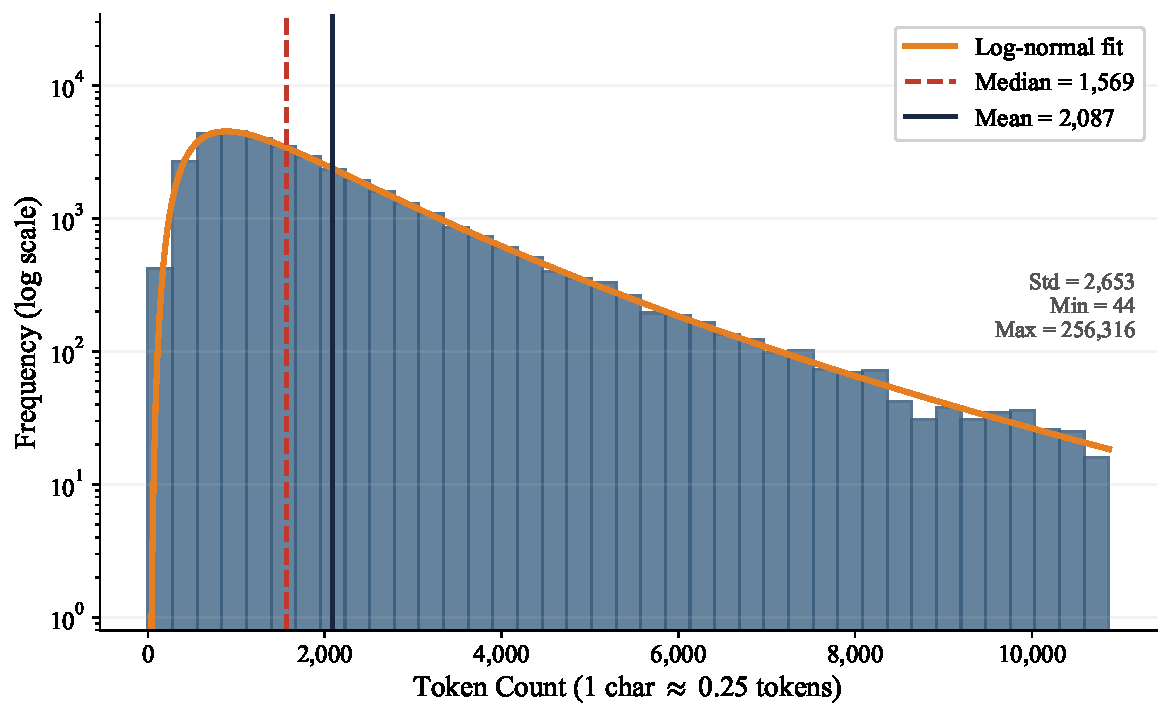
\includegraphics[width=0.8\columnwidth]{figs/figure1_skillmd_distribution.pdf}}
    
%     \caption{Token distribution of SKILL.md files (n=\num{36338}, 99.5th percentile shown). Most Skills are lightweight with median $\sim$1.5k tokens.}
%     \label{fig:skill_md_length}
%   \end{center}
%   \vskip -0.1in
% \end{figure}

% \begin{figure}[ht]
%   \vskip 0.1in
%   \begin{center}
%     %\centerline{\includegraphics[width=0.8\columnwidth]{figs/total_char_length_distribution.png}}
%     \centerline{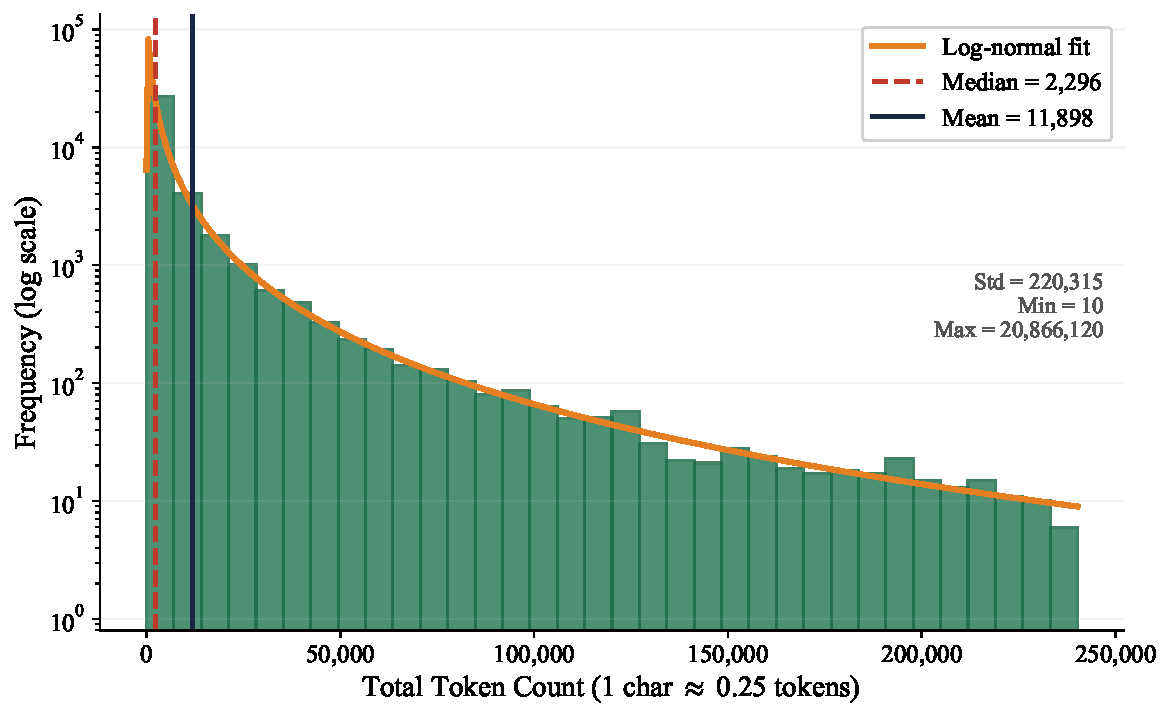
\includegraphics[width=0.8\columnwidth]{figs/figure2_total_distribution.pdf}}
%     \caption{Total Skill size distribution (excluding metadata.json, n=\num{37078}, 99.5th percentile shown). Median total size remains under 2.5k tokens, with distribution highly skewed toward concise artifacts.}
%     \label{fig:total_length}
%   \end{center}
%   \vskip -0.1in
% \end{figure}

% \paragraph{Domain Coverage.}
% Skills span diverse domains (Figure~\ref{fig:category}):
% \begin{itemize}
%     \item Software Development: 38\% (git workflows, code review, testing)
%     \item Data Analysis: 22\% (pandas, SQL, visualization)
%     \item DevOps/Infrastructure: 15\% (Docker, Kubernetes, CI/CD)
%     \item Writing/Documentation: 12\% (technical writing, API docs)
%     \item Other: 13\% (scientific computing, finance, etc.)
% \end{itemize}

% \begin{figure}[ht]
%   \vskip 0.1in
%   \begin{center}
%     \centerline{\includegraphics[width=0.8\columnwidth]{figs/category.png}}
%     \caption{Category distribution of Skills. No single category dominates; Skills are spread across documentation, version control, code quality, CLI tools, DevOps, APIs, and frontend tasks.}
%     \label{fig:category}
%   \end{center}
%   \vskip -0.1in
% \end{figure}

% \paragraph{Structural Patterns.}
% Most Skills (78\%) follow the standard structure with SKILL.md plus optional resources.
% Figure~\ref{fig:file_count} shows that most Skills contain very few files (median of one, concentrated below five). Figure~\ref{fig:file_extension} confirms the ecosystem is documentation-heavy: markdown files dominate, followed by scripting and configuration code.

% \begin{figure}[ht]
%   \vskip 0.1in
%   \begin{center}
%     \centerline{\includegraphics[width=0.8\columnwidth]{figs/file_count_distribution.png}}
%     \caption{File count distribution per Skill. Most Skills contain 1--5 files.}
%     \label{fig:file_count}
%   \end{center}
%   \vskip -0.1in
% \end{figure}

% \begin{figure}[ht]
%   \vskip 0.1in
%   \begin{center}
%     \centerline{\includegraphics[width=0.8\columnwidth]{figs/file_extension_distribution.png}}
%     \caption{File extension distribution. Markdown files dominate, indicating Skills prioritize natural-language instructions over executable implementations.}
%     \label{fig:file_extension}
%   \end{center}
%   \vskip -0.1in
% \end{figure}

% \subsection{Quality Indicators}

% We developed a quality scoring rubric based on:
% \begin{enumerate}
%     \item \textbf{Completeness:} Presence of required components (0--3 points)
%     \item \textbf{Clarity:} Readability and organization (0--3 points)
%     \item \textbf{Specificity:} Actionable vs.\ vague guidance (0--3 points)
%     \item \textbf{Examples:} Presence and quality of examples (0--3 points)
% \end{enumerate}

% Mean quality score across the ecosystem is 6.2/12 (SD=2.8), indicating substantial room for improvement in Skill authoring practices.

% \subsection{Implications for Benchmark Design}

% This ecosystem analysis directly informed \benchmarkName{} construction:
% \begin{itemize}
%     \item \textbf{Domain selection:} Task categories mirror ecosystem coverage, ensuring Skills exist for evaluation
%     \item \textbf{Quality awareness:} Ecosystem mean quality of 6.2/12 motivated our leakage audit and authoring guidelines---low-quality Skills would confound efficacy measurement
%     \item \textbf{Skill selection:} We selected benchmark Skills from the top quality quartile (score $\geq$ 9/12) to isolate the effect of procedural knowledge from Skill quality variance
%     \item \textbf{Size constraints:} Median Skill size ($\sim$800 tokens) informed our 8K context budget allocation
% \end{itemize}

% \paragraph{Limitation: Benchmark vs.\ Ecosystem Gap.}
% Our 85 curated tasks with high-quality Skills represent an optimistic scenario.
% Real-world Skill usage involves lower-quality Skills (ecosystem mean: 6.2/12 vs.\ benchmark mean: 10.1/12) and imperfect Skill-task matching.
% Future work should evaluate with ecosystem-representative Skill samples.


% \section{Qualitative Case Studies}
% \label{app:cases}

% We present three case studies illustrating Skill efficacy patterns.

% \subsection{Case 1: Successful Skill Application}

% \textbf{Task:} Fix a failing CI pipeline in a Python repository (Medium difficulty, DevOps domain).

% \textbf{Skill:} \texttt{ci-debugging} --- provides systematic debugging workflow: (1) check logs, (2) identify failing step, (3) reproduce locally, (4) trace dependencies.

% \textbf{Vanilla trajectory (GPT-5.2):} Agent immediately attempts to modify \texttt{.github/workflows/main.yml} based on error message, introduces syntax error, enters retry loop, times out after 47 minutes.

% \textbf{Skill-augmented trajectory:} Agent follows Skill procedure---reads full log, identifies dependency version conflict, checks \texttt{requirements.txt}, finds pinned version incompatibility, updates version constraint, verifies fix locally before committing. Completes in 12 minutes.

% \textbf{Analysis:} Skill provided systematic procedure that prevented premature action. Key Skill component: explicit ``reproduce locally before modifying'' instruction.

% \subsection{Case 2: Skill Present but Ignored}

% \textbf{Task:} Implement OAuth authentication flow (Hard difficulty, Software Engineering domain).

% \textbf{Skill:} \texttt{oauth-integration} --- provides flow diagram, common pitfalls, security checklist.

% \textbf{Trajectory (Claude Haiku 4.5):} Agent acknowledges Skill in first response (``I'll follow the oauth-integration guidelines...'') but subsequently ignores security checklist, implements vulnerable token storage, fails verification.

% \textbf{Analysis:} Skill was recognized but not operationalized. Smaller models may lack capacity to maintain Skill guidance across long trajectories. Suggests need for Skill-aware prompting strategies.

% \subsection{Case 3: Skill Quality Impact}

% \textbf{Task:} Configure Kubernetes deployment (Medium difficulty, DevOps domain).

% \textbf{Skill A (high quality, score 11/12):} Step-by-step procedure with YAML examples, common errors, verification commands.

% \textbf{Skill B (low quality, score 5/12):} High-level overview, no examples, vague guidance (``configure the deployment appropriately'').

% \textbf{Results (Claude Sonnet 4.5):} Skill A: 87.5\% pass rate. Skill B: 54.2\% pass rate (below vanilla: 58.3\%).

% \textbf{Analysis:} Low-quality Skills can hurt performance by consuming context budget without providing actionable guidance. Highlights importance of Skill quality control.


% \section{Additional Experimental Details}
% \label{app:details}

% \subsection{Context Usage Analysis}

% Table~\ref{tab:context_full} provides detailed context usage statistics by condition.

% \begin{table}[ht]
% \centering
% \caption{Detailed context usage by Skill condition.}
% \label{tab:context_full}
% \begin{tabular}{lccccc}
% \toprule
% \textbf{Metric} & \textbf{L0} & \textbf{L1} & \textbf{L2} & \textbf{L3} & \textbf{BYOS} \\
% \midrule
% Mean tokens & \num{4821} & \num{5102} & \num{5487} & \num{6142} & \num{5891} \\
% Std. dev. & \num{1203} & \num{1342} & \num{1518} & \num{1847} & \num{1723} \\
% Truncation rate & 8.3\% & 9.7\% & 11.4\% & 14.2\% & 13.1\% \\
% \bottomrule
% \end{tabular}
% \end{table}

% \subsection{Skill Injection Format}

% Skills are injected as system-level context with the following structure:

% \begin{verbatim}
% <skill name="[NAME]">
%   <instructions>[SKILL.md content]</instructions>
%   <resources>[file list]</resources>
% </skill>

% [Task instruction follows]
% \end{verbatim}

% \subsection{Confidence Interval Calculation}

% We compute 95\% confidence intervals using the percentile bootstrap method with 1000 resamples.
% For normalized gain, we compute CIs on the gain metric directly rather than on the component pass rates.

% \subsection{10-Run Validation}

% For a subset of configurations (GPT-5.2 and Claude Opus 4.5, all 27 hard tasks, L0 and L3 conditions), we conducted 10 runs instead of 3. Results show:
% \begin{itemize}
%     \item Mean $\Delta$ within 1.2pp of 3-run estimates
%     \item Standard error reduced by $\sim$45\%
%     \item All conclusions remain unchanged
% \end{itemize}

% This validates that 3 runs provides sufficient precision for our main findings.


% \section{Reproducibility Checklist}
% \label{app:reproducibility}

% \begin{itemize}
%     \item[$\square$] Code and evaluation scripts will be released
%     \item[$\square$] Task specifications with Dockerfiles provided
%     \item[$\square$] All Skills used in evaluation documented
%     \item[$\square$] Model API versions and settings specified
%     \item[$\square$] Random seeds and determinism settings documented
%     \item[$\square$] Complete results tables in supplementary materials
% \end{itemize}

% %%%%%%%%%%%%%%%%%%%%%%%%%%%%%%%%%%%%%%%%%%%%%%%%%%%%%%%%%%%%%%%%%%%%%%%%%%%%%%%
% %%%%%%%%%%%%%%%%%%%%%%%%%%%%%%%%%%%%%%%%%%%%%%%%%%%%%%%%%%%%%%%%%%%%%%%%%%%%%%%

% \end{document}
